% ******************************* PhD Thesis Template **************************
% Please have a look at the README.md file for info on how to use the template

\documentclass[a4paper,12pt,times,numbered,print,index]{Classes/PhDThesisPSnPDF}

% ******************************************************************************
% ******************************* Class Options ********************************
% *********************** See README for more details **************************
% ******************************************************************************

% `a4paper'(The University of Cambridge PhD thesis guidelines recommends a page
% size a4 - default option) or `a5paper': A5 Paper size is also allowed as per
% the Cambridge University Engineering Deparment guidelines for PhD thesis
%
% `11pt' or `12pt'(default): Font Size 10pt is NOT recommended by the University
% guidelines
%
% `oneside' or `twoside'(default): Printing double side (twoside) or single
% side.
%
% `print': Use `print' for print version with appropriate margins and page
% layout. Leaving the options field blank will activate Online version.
%
% `index': For index at the end of the thesis
%
% `draftclassic': For draft mode without loading any images (same as draft in book)
%
% `draft': Special draft mode with line numbers, images, and water mark with
% timestamp and custom text. Position of the text can also be modified.
%
% `abstract': To generate only the title page and abstract page with
% dissertation title and name, to submit to the Student Registry
%
% `chapter`: This option enables only the specified chapter and it's references
%  Useful for review and corrections.
%
% ************************* Custom Page Margins ********************************
%
% `custommargin`: Use `custommargin' in options to activate custom page margins,
% which can be defined in the preamble.tex. Custom margin will override
% print/online margin setup.
%
% *********************** Choosing the Fonts in Class Options ******************
%
% `times' : Times font with math support. (The Cambridge University guidelines
% recommend using times)
%
% `fourier': Utopia Font with Fourier Math font (Font has to be installed)
%            It's a free font.
%
% `customfont': Use `customfont' option in the document class and load the
% package in the preamble.tex
%
% default or leave empty: `Latin Modern' font will be loaded.
%
% ********************** Choosing the Bibliography style ***********************
%
% `authoryear': For author-year citation eg., Krishna (2013)
%
% `numbered': (Default Option) For numbered and sorted citation e.g., [1,5,2]
%
% `custombib': Define your own bibliography style in the `preamble.tex' file.
%              `\RequirePackage[square, sort, numbers, authoryear]{natbib}'.
%              This can be also used to load biblatex instead of natbib
%              (See Preamble)
%
% **************************** Choosing the Page Style *************************
%
% `default (leave empty)': For Page Numbers in Header (Left Even, Right Odd) and
% Chapter Name in Header (Right Even) and Section Name (Left Odd). Blank Footer.
%
% `PageStyleI': Chapter Name next & Page Number on Even Side (Left Even).
% Section Name & Page Number in Header on Odd Side (Right Odd). Footer is empty.
%
% `PageStyleII': Chapter Name on Even Side (Left Even) in Header. Section Number
% and Section Name in Header on Odd Side (Right Odd). Page numbering in footer

% Uncomment to change page style
%\pagestyle{PageStyleII}


% ********************************** Preamble **********************************
% Preamble: Contains packages and user-defined commands and settings
% ******************************************************************************
% ****************************** Custom Margin *********************************

% Add `custommargin' in the document class options to use this section
% Set {innerside margin / outerside margin / topmargin / bottom margin}  and
% other page dimensions
\ifsetCustomMargin
  \RequirePackage[left=37mm,right=30mm,top=35mm,bottom=30mm]{geometry}
  \setFancyHdr % To apply fancy header after geometry package is loaded
\fi

% Add spaces between paragraphs
%\setlength{\parskip}{0.5em}
% Ragged bottom avoids extra whitespaces between paragraphs
\raggedbottom
% To remove the excess top spacing for enumeration, list and description
%\usepackage{enumitem}
%\setlist[enumerate,itemize,description]{topsep=0em}

% *****************************************************************************
% ******************* Fonts (like different typewriter fonts etc.)*************

% Add `customfont' in the document class option to use this section

\ifsetCustomFont
  % Set your custom font here and use `customfont' in options. Leave empty to
  % load computer modern font (default LaTeX font).
  %\RequirePackage{helvet}

  % For use with XeLaTeX
  %  \setmainfont[
  %    Path              = ./libertine/opentype/,
  %    Extension         = .otf,
  %    UprightFont = LinLibertine_R,
  %    BoldFont = LinLibertine_RZ, % Linux Libertine O Regular Semibold
  %    ItalicFont = LinLibertine_RI,
  %    BoldItalicFont = LinLibertine_RZI, % Linux Libertine O Regular Semibold Italic
  %  ]
  %  {libertine}
  %  % load font from system font
  %  \newfontfamily\libertinesystemfont{Linux Libertine O}
\fi

% *****************************************************************************
% **************************** Custom Packages ********************************

% ************************* Algorithms and Pseudocode **************************

%\usepackage{algpseudocode}


% ********************Captions and Hyperreferencing / URL **********************

% Captions: This makes captions of figures use a boldfaced small font.
%\RequirePackage[small,bf]{caption}

\RequirePackage[labelsep=space,tableposition=top]{caption}
\renewcommand{\figurename}{Fig.} %to support older versions of captions.sty


% *************************** Graphics and figures *****************************

%\usepackage{rotating}
%\usepackage{wrapfig}

% Uncomment the following two lines to force Latex to place the figure.
% Use [H] when including graphics. Note 'H' instead of 'h'
%\usepackage{float}
%\restylefloat{figure}

% Subcaption package is also available in the sty folder you can use that by
% uncommenting the following line
% This is for people stuck with older versions of texlive
%\usepackage{sty/caption/subcaption}
\usepackage{subcaption}

% ********************************** Tables ************************************
\usepackage{booktabs} % For professional looking tables
\usepackage{multirow}

%\usepackage{multicol}
%\usepackage{longtable}
%\usepackage{tabularx}


% *********************************** SI Units *********************************
\usepackage{siunitx} % use this package module for SI units


% ******************************* Line Spacing *********************************

% Choose linespacing as appropriate. Default is one-half line spacing as per the
% University guidelines

% \doublespacing
% \onehalfspacing
% \singlespacing


% ************************ Formatting / Footnote *******************************

% Don't break enumeration (etc.) across pages in an ugly manner (default 10000)
%\clubpenalty=500
%\widowpenalty=500

%\usepackage[perpage]{footmisc} %Range of footnote options


% *****************************************************************************
% *************************** Bibliography  and References ********************

%\usepackage{cleveref} %Referencing without need to explicitly state fig /table

% Add `custombib' in the document class option to use this section
\ifuseCustomBib
   \RequirePackage[square, sort, numbers, authoryear]{natbib} % CustomBib

% If you would like to use biblatex for your reference management, as opposed to the default `natbibpackage` pass the option `custombib` in the document class. Comment out the previous line to make sure you don't load the natbib package. Uncomment the following lines and specify the location of references.bib file

%\RequirePackage[backend=biber, style=numeric-comp, citestyle=numeric, sorting=nty, natbib=true]{biblatex}
%\addbibresource{References/references} %Location of references.bib only for biblatex, Do not omit the .bib extension from the filename.

\fi

% changes the default name `Bibliography` -> `References'
\renewcommand{\bibname}{References}


% ******************************************************************************
% ************************* User Defined Commands ******************************
% ******************************************************************************

% *********** To change the name of Table of Contents / LOF and LOT ************

%\renewcommand{\contentsname}{My Table of Contents}
%\renewcommand{\listfigurename}{My List of Figures}
%\renewcommand{\listtablename}{My List of Tables}


% ********************** TOC depth and numbering depth *************************

\setcounter{secnumdepth}{2}
\setcounter{tocdepth}{2}


% ******************************* Nomenclature *********************************

% To change the name of the Nomenclature section, uncomment the following line

%\renewcommand{\nomname}{Symbols}


% ********************************* Appendix ***********************************

% The default value of both \appendixtocname and \appendixpagename is `Appendices'. These names can all be changed via:

%\renewcommand{\appendixtocname}{List of appendices}
%\renewcommand{\appendixname}{Appndx}

% *********************** Configure Draft Mode **********************************

% Uncomment to disable figures in `draft'
%\setkeys{Gin}{draft=true}  % set draft to false to enable figures in `draft'

% These options are active only during the draft mode
% Default text is "Draft"
%\SetDraftText{DRAFT}

% Default Watermark location is top. Location (top/bottom)
%\SetDraftWMPosition{bottom}

% Draft Version - default is v1.0
%\SetDraftVersion{v1.1}

% Draft Text grayscale value (should be between 0-black and 1-white)
% Default value is 0.75
%\SetDraftGrayScale{0.8}


% ******************************** Todo Notes **********************************
%% Uncomment the following lines to have todonotes.

%\ifsetDraft
%	\usepackage[colorinlistoftodos]{todonotes}
%	\newcommand{\mynote}[1]{\todo[author=kks32,size=\small,inline,color=green!40]{#1}}
%\else
%	\newcommand{\mynote}[1]{}
%	\newcommand{\listoftodos}{}
%\fi

% Example todo: \mynote{Hey! I have a note}

% *****************************************************************************
% ******************* Better enumeration my MB*************
\usepackage{enumitem}



% Wuhyun settings
\usepackage{amsmath}
\usepackage{amssymb}

\newcommand{\Lagr}{\mathcal{L}}

% ************************ Thesis Information & Meta-data **********************
% Thesis title and author information, refernce file for biblatex
% ************************ Thesis Information & Meta-data **********************
%% The title of the thesis
\title{High-resolution CMB bispectrum estimator}
%\texorpdfstring is used for PDF metadata. Usage:
%\texorpdfstring{LaTeX_Version}{PDF Version (non-latex)} eg.,
%\texorpdfstring{$sigma$}{sigma}

%% Subtitle (Optional)
%\subtitle{Using the CUED template}

%% The full name of the author
\author{Wu Hyun Sohn}

%% Department (eg. Department of Engineering, Maths, Physics)
\dept{Department of Applied Mathematics and Theoretical Physics}

%% University and Crest
\university{University of Cambridge}
% Crest minimum should be 30mm.
\crest{
\includegraphics[width=0.2\textwidth]{University_Crest}}
%% Use this crest, if you are using the college crest
%% Crest long miminum should be 65mm
%\crest{
\includegraphics[width=0.45\textwidth]{University_Crest_Long}}

%% College shield [optional] 
% Crest minimum should be 30mm.
%\collegeshield{
\includegraphics[width=0.2\textwidth]{CollegeShields/Kings}}


%% Supervisor (optional)
%% for multiple supervisors, append each supervisor with the \newline command
%\supervisor{Prof. A.B. Supervisor\newline
%Prof. C.D. Supervisor}

%% Supervisor Role (optional) - Supervisor (default) or advisor
% \supervisorrole{\textbf{Supervisors: }}
%% if no title is desired:
% \supervisorrole{}

%% Supervisor line width: required to align supervisors
%\supervisorlinewidth{0.35\textwidth}

%% Advisor (optional)
%% for multiple advisors, append each advisor with the \newline command
%\advisor{Dr. A. Advisor\newline
%Dr. B. Advisor}
     
%% Advisor Role (optional) - Advisor (default) or leave empty
% \advisorrole{Advisors: }
%% if no title is required
% \advisorrole{}

%% Advisor line width: required to align supervisors
%\advisorlinewidth{0.25\textwidth}


%% You can redefine the submission text:
% Default as per the University guidelines:
% ``This dissertation is submitted for the degree of''
%\renewcommand{\submissiontext}{change the default text here if needed}

%% Full title of the Degree
\degreetitle{Doctor of Philosophy}

%% College affiliation (optional)
\college{Trinity College}

%% Submission date
% Default is set as {\monthname[\the\month]\space\the\year}
%\degreedate{September 2014} 

%% Meta information
\subject{LaTeX} \keywords{{LaTeX} {PhD Thesis} {Engineering} {University of
Cambridge}}


% ***************************** Abstract Separate ******************************
% To printout only the titlepage and the abstract with the PhD title and the
% author name for submission to the Student Registry, use the `abstract' option in
% the document class.

\ifdefineAbstract
 \pagestyle{empty}
 \includeonly{Declaration/declaration, Abstract/abstract}
\fi

% ***************************** Chapter Mode ***********************************
% The chapter mode allows user to only print particular chapters with references
% Title, Contents, Frontmatter are disabled by default
% Useful option to review a particular chapter or to send it to supervisior.
% To use choose `chapter' option in the document class

% \ifdefineChapter
% \includeonly{Chapter3/chapter3}
% \fi

% ******************************** Front Matter ********************************
\begin{document}

\frontmatter

\maketitle

%% ******************************* Thesis Dedidcation ********************************

\begin{dedication} 

I would like to dedicate this thesis to my loving family \dots

\end{dedication}


% ******************************* Thesis Declaration ***************************

\begin{declaration}

I hereby declare that except where specific reference is made to the work of 
others, the contents of this dissertation are original and have not been 
submitted in whole or in part for consideration for any other degree or 
qualification in this, or any other university. This dissertation is my own 
work and contains nothing which is the outcome of work done in collaboration 
with others, except as specified in the text and Acknowledgements. This 
dissertation contains fewer than 65,000 words including appendices, 
bibliography, footnotes, tables and equations and has fewer than 150 figures.

% Author and date will be inserted automatically from thesis.tex \author \degreedate

\end{declaration}


%% ************************** Thesis Acknowledgements **************************

\begin{acknowledgements}      

If this thesis was to be shared between everyone who contributed to making it happen, my own share would be about a page... I would like to use this page to thank them.


\end{acknowledgements}

% ************************** Thesis Abstract *****************************
% Use `abstract' as an option in the document class to print only the titlepage and the abstract.
\begin{abstract}

The Cosmic Microwave Background (CMB) is one of the most valuable probes of the universe we have today. Anisotropies present in the ancient light contain rich statistical information about the perturbations in the early universe and their subsequent evolution until now. CMB bispectrum, the Fourier equivalent of three-point correlation function, allows us to study weak non-Gaussian signatures of the primordial fluctuations. Primordial non-Gaussianity is a key prediction of many physically well-motivated inflation models, and measuring its shape and amplitude allows us to constrain them.

This thesis comprises two sections. In the first section, we present forecasts on primordial non-Gaussianity constraints from upcoming CMB Stage-4 surveys. We focus our attention to models favoured by the Planck analysis, where a sharp feature in either the inflationary potential or sound speed causes oscillations in the bispectrum. Using preliminary specifications, we find that the Simons Observatory will have up to a factor of 1.6 improvements over Planck, increased to 1.7-2.2 for CMB Stage-4 experiments. Motivated by bright prospects, we developed a novel CMB bispectrum estimator suited for the resolution and sensitivity of future surveys.

We discuss our high-resolution bispectrum estimator in the second section. Our code, named CMB-BEst, utilises a set of general basis functions to accurately constrain a wide variety of models. Implementing such flexible and precise estimator was a computationally challenging task. We detail our algorithm design, code optimisation and parallelisation for high performance computing clusters, which made this very challenging computation tractable. Validation tests, both for internal consistency and comparisons against conventional estimators are provided, together with a proof-of-concept application. We highlight how CMB-BEst can be used for both general and targeted analyses of previously unconstrained models.

\end{abstract}


% *********************** Adding TOC and List of Figures ***********************

\tableofcontents

\listoffigures

\listoftables

% \printnomenclature[space] space can be set as 2em between symbol and description
%\printnomenclature[3em]

\printnomenclature

% ******************************** Main Matter *********************************
\mainmatter

%!TEX root = ../thesis.tex
%*******************************************************************************
%*********************************** First Chapter *****************************
%*******************************************************************************

\chapter{Introduction}

\ifpdf
    \graphicspath{{Chapter1/Figs/Raster/}{Chapter1/Figs/PDF/}{Chapter1/Figs/}}
\else
    \graphicspath{{Chapter1/Figs/Vector/}{Chapter1/Figs/}}
\fi


%********************************** %First Section  **************************************
\section{From background to foreground}

New outline:
- GR. Statistical homogeneity and isotropy -> FLRW metric. No static solution.

- Hubble's results. Expanding universe -> Big Bang.

- Discovery of CMB. CMB is a key prediction of Big Bang theory

- Big Bang theory's problem with initial conditions. Inflation. Quantum fluctuations as seeds for inhomogeneities of the universe.

- CMB anisotropy, 1 in $10^5$. Consistent with inflationary predictions.

- Observational evidence for dark energy and dark matter. Emergence of inflationary LCDM.

- LCDM successful. Planck CMB power spectrum -> consistent and measures parameters to percent level. Era of precision cosmology.

- Quick summary of CMB's usefulness! Its existence, anisotropy and spectrum all contributed...  CMB probes initial conditions, growth of the universe and matter distribution (through lensing).

- Next big question - inflation's mechanism? Primordial non-Gaussianity is a robust prediction of many models. Three-point correlation function as a key statistic for differentiation.

- CMB bispectrum. Planck gave a lot of insight. No detection, but oscillatory models are of interest. Main challenge - computational complexity.

- Next generation of CMB experiments upcoming. Polarisation sensitivity improved, higher resolution. Need for development of new, improved pipeline capable of dealing with high resolution data.

- Thesis organisation.

Radio astronomers Arno Penzias and Robert Wilson were calibrating their 50-feet-long horn antenna when they found a mysterious background noise. The measurements were independent of time and location in the sky, and persisted after the removal of various potential contaminants. After the theoretical work of Robert Dicke, Jim Peebles, and David Wilkinson was brought forward \cite{Dicke1965}, Penzias and Wilson identified the noise as cosmic microwave background radiation (CMB): ancient light from the early universe reaching us after billions of years \cite{Penzias1965}. The discovery provided us with one of the most valuable probes of the physical universe, leading to major development in observational cosmology.

On the theoretical side, modern mathematical formulation of cosmology owes to Einstein's work on general relativity in 1915. Using his framework, Friedmann, Lemaître, Robertson, and Walker contributed to writing down the unique metric for spatially homogeneous and isotropic universe. The FLRW metric dictates growth of the universe from the Big Bang to present day. Such expansion of the universe was supported by Edwin Hubble's measurements of Cepheid variables and redshift (add year), as well as the aforementioned discovery of CMB. What is widely accepted to be the standard model of modern cosmology, the $\Lambda$CDM model, appeared only in the late 1990s. The six-parameter model assumes presence of cold dark matter and dark energy, in addition to baryons and radiation, as main contributors to the total energy density of the universe.

The $\Lambda$CDM model has been extremely successful in explaining modern cosmological observations. CMB measurements from \textit{Planck} satellite, in particular, show exceptional agreement with the model. Planck was a space observatory developed by the European Space Agency. The Planck satellite observed the CMB in nine frequency bands from 2009 to 2013, with resolution and sensitivity substantially improved compared to its predecessor - the Wilkinson Microwave Anisotropy Probe (WMAP). Able to resolve CMB anisotropy in much smaller scale, Planck placed one of the most stringent bounds on the theoretical parameters of $\Lambda$CDM so far.

How does CMB contain so much information about the universe? The answer is twofold. First is due to the fact that CMB anisotropy originates from primordial perturbations. Statistical properties of the initial fluctuations can be deduced from analysing correlation functions of the CMB, letting us constrain the early universe physics. Second reason is that CMB tracks history of the universe as it travels from the background to our foreground. CMB photons scatter with baryons before free-streaming all the way to our foreground, which then experience both growth of the universe and gravitational potential of matter perturbations. These signatures are engraved in CMB anisotropy spectrum, redshift, and weak lensing.

The CMB anisotropy is observed to be nearly Gaussian distributed. Statistical characteristics of a Gaussian random field can be summarised entirely using two-point correlation functions, or their Fourier counterpart: power spectrum. The CMB power spectra have been thoroughly studied to constrain various cosmological parameters. Meanwhile, higher-order statistics such as three-point correlation functions (bispectrum in Fourier space) also contain valuable information about our universe. They probe non-Gaussian statistics of the CMB arising from both primordial origin and late-time effects.

Primordial non-Gaussianity is a key statistic for studying physics of the early universe. The theory of inflation has been successful in describing the observed data, but its exact mechanism is yet undetermined. Currently there are numerous viable inflationary models with well-founded physical motivations. Non-Gaussian signatures of primordial fluctuations are robust predictions of various models, and measuring their shape and amplitude allows us to constrain inflationary scenario. CMB bispectrum analysis from Planck yielded the most precise measurements of primordial non-Gaussianity to date. So far, no statistically significant amount of non-Gaussianity has been detected.

In the near future, we expect several new major CMB experiments. Simons Observatory (SO) is a ground-based experiment currently under construction in the Atacama Desert of Chile. SO is expected to measure both CMB temperature and polarisation to unprecedented precision, largely improved compared to Planck. The first light from SO is planned to be observed in early 2022. Many more CMB Stage-4 (CMB-S4) experiments are proposed, brightening future prospects for CMB. In particular, the upcoming measurements will allow us to constrain primordial non-Gaussianity further, providing discovery potential.

This thesis is organised as follows. In Chapter 1, we review the standard formulation of cosmology, deriving the form of scale factor in homogeneous universe. Motivation and formalism of slow-roll inflation is also presented here. Chapter 2 details cosmological perturbation theory, with a focus on the CMB anisotropy. We summarise methods for computing the transfer function of CMB, and introduce the concept of CMB polarisation. Next, in Chapter 3 we define bispectrum and discuss how it can be used to probe primordial non-Gaussianity. An example of single-field inflation with non-canonical kinetic term will be provided to demonstrate computation of non-Gaussianity using the in-in formalism.

Chapter 4 and 5 contain my original work, based on research conducted in collaboration with my supervisor James Fergusson. Chapter 4 contains the forecast for future CMB-S4 surveys on the primordial non-Gaussianity parameter $f_{NL}$. SO experiment specifications and expected CMB-S4 setup were used to predict their improved constraints via Fisher information analysis. We focussed on models with oscillatory features, where steep enhancement in polarisation sensitivity greatly benefit constraining power.

Motivated by the positive prospects from forecasts detailed in Chapter 4, we worked on developing a high-resolution bispectrum estimation pipeline suitable for future surveys. Chapter 5 contains formulation and development details of the developed program, as well as consistency checks from the thorough verification process. We outline the benefits of new pipeline compared to conventional methods, and present some working examples. Lastly, Chapter 6 concludes the thesis by summarising and presenting plans for future research.

\section{The homogeneous universe}

In this section we review the standard cosmological formulation for the homogeneous universe, neglecting any perturbations. What we derive here will serve as a background solution for the full perturbative result discussed in the next chapter. We assume general relativity to be an accurate theory of gravity for relevant scales.

\subsection{Geometry}

In general relativity, spacetime is represented by a 4-dimensional Lorentzian manifold equipped with a metric. Distance measure in curved spacetime is given by the metric tensor $g$;
\begin{align}
	ds^2 \,=\, g_{\mu \nu} \; dx^\mu dx^\nu	,
\end{align}
where the Greek letters $\mu, \nu = 0,1,2,3$ represent time ($0$) and spatial ($1,2,3$) indices of local coordinates. Flat spacetime has metric $g_{\mu\nu} = \eta_{\mu\nu} = \text{diag}\{-1, 1, 1, 1\}$, also known as the Minkowski metric. Throughout this thesis we adopt the sign convention $(-, +, +, +)$ and work in units where $c=1$. Unless specified otherwise, the Einstein summation convention is assumed. 

In curved spacetime, free particles follow a trajectory given by the geodesic equation;
\begin{align}
	\frac{d^2x^\mu}{ds^2} \,+\, \Gamma^\mu_{\nu \rho} \frac{dx^\nu}{ds} \frac{dx^\rho}{ds} \,=\, 0,  \label{eqn:geodesic}
\end{align}
with $s$ an affine parameter parametrising the trajectory, and $\Gamma^\mu_{\nu\rho}$ the Christoffel symbol representing metric connection. Its value is given in terms of the metric tensor by
\begin{align}
	\Gamma^{\mu}_{\nu\rho} \,=\, \frac{1}{2}~ g^{\mu\sigma} \left( \partial_\rho g_{\nu\sigma} \,+\, \partial_\nu g_{\rho\sigma} \,-\, \partial_\sigma g_{\nu\rho}  \right). \label{def:Levi_Civita}
\end{align}
Here and throughout this thesis, $\partial_\mu$ denote the partial derivative with respect to local coordinate $x^\mu$. Note $g^{\nu\sigma}$ is the inverse metric satisfying $g^{\mu\nu} g_{\nu\rho} \,=\, \delta^\nu_\rho$.

Defining tangent vector as $U^\mu = dx^\mu / ds$, the equation can be rewritten in a covariant form given by
\begin{align}
	\left( \nabla_U U \right)^a \,=\, U^b \nabla_b U^a \,=\, 0.
\end{align}
We follow the convention where Roman letters are used for abstract indices. Note that in terms of local coordinates, the covariant derivative of a vector field is defined as $\nabla_\nu U^\mu = \partial_\nu U^\mu + \Gamma^\mu_{\nu\rho} U^\rho$.

Distance between two geodesics that are initially parallel may change in curved spacetime. Such geometric information is encapsulated within the Riemann curvature tensor $R^a_{bcd}$. \footnote{Consider a 1-parameter family of geodesics $\gamma(s,t)$, where $t$ is an affine parameter. The geodesic deviation equation states $T^\rho \nabla_\rho ( T^\nu \nabla_\nu S^\mu ) = R^\mu_{\nu\rho\sigma} T^\nu T^\rho S^\sigma$, where tangent vectors $T=\partial/\partial t$, $S=\partial/\partial s$.} From $R^a_{bcd}$ we can evaluate the Ricci curvature tensor $R_{ab}$, the Ricci scalar $R$, and finally the Einstein tensor $G_{ab}$. They are defined as follows.
\begin{align}
	R^\mu_{\nu\rho\sigma} \,:=& \,\, \partial_\rho \Gamma^\mu_{\nu\sigma} \,-\, \partial_\sigma \Gamma^\mu_{\nu\rho} \,+\, \Gamma^\tau_{\nu\sigma} \Gamma^\mu_{\tau\rho} \,-\, \Gamma^\tau_{\nu\rho} \Gamma^\mu_{\tau\sigma}  \label{def:Riemann_tensor}\\
	R_{\mu\nu} \,:=& \,\, R^\rho_{\mu\rho\nu}  \\ % Extra detail: \,=\, \partial_\rho \Gamma^\rho_{\mu\nu} \,-\, \partial_\nu \Gamma^\rho_{\mu\rho} \,+\, \Gamma^\tau_{\mu\nu} \Gamma^\rho_{\tau\rho} \,-\, \Gamma^\tau_{\mu\rho} \Gamma^\rho_{\tau\nu}
	R \,:=& \,\, g^{\mu\nu} R_{\mu\nu} \\
	G_{\mu\nu} \,:=& \,\, R_{\mu\nu} - \frac{1}{2} g_{\mu\nu} R \label{def:Einstein_tensor}
\end{align}

The Einstein tensor is symmetric, i.e. $G_{\mu\nu} = G_{\nu\mu}$. It is also important to note that its divergence vanishes; $\nabla^\mu G_{\mu\nu} = 0$, which can be proven using the contracted Bianchi identity.


\subsection{The FLRW universe}
On very large scales, our universe is observed to be uniform in space (homogeneous) and not have a favoured direction (isotropic). Spatial part of the homogeneous and isotropic metric has constant curvature and can be categorised into three: spherical ($\mathbb{S}^3$), Euclidean ($\mathbb{E}^3$), and hyperbolic ($\mathbb{H}^3$). They are induced from embedding $\mathbb{R}^3$ into submanifolds of $\mathbb{R}^4$ equipped with the Euclidean metric, defined as $K|\mathbf{x}|^2 + u^2 = 1$. Here $K=1,0,-1$ for $\mathbb{S}^3$, $\mathbb{E}^3$, and $\mathbb{H}^3$, respectively. Writing the embedding as $f: x^i = (x,y,z) \mapsto X^I =(x,y,z,\sqrt{1-K(x^2+y^2+z^2)})$, the induced metric
\begin{align}
	\gamma_{ij} := \frac{\partial X^I}{\partial x^i} \frac{\partial X^J}{\partial x^j} \delta_{IJ}
	= \delta_{ij} + \frac{x_i x_j}{1-Kx_k x^k}. \label{eqn:FLRW_metric_spatial}
\end{align}
The spatial line element is therefore given by
\begin{align}
	dl^2 = \gamma_{ij} dx^i dx^j =& d\mathbf{x} \cdot d\mathbf{x} + \frac{K(\mathbf{x} \cdot d\mathbf{x})^2}{1-K (\mathbf{x} \cdot \mathbf{x})} \\
	=& \frac{1}{1-Kr^2} dr^2 + r^2 d\Omega^2,
\end{align}
where the angular line element $d\Omega^2 = d\theta^2 + \sin^2\theta d\phi^2$.

We may now write down the form of the metric describing our universe in large scales;
\begin{align}
	ds^2 = - dt^2 + a(t)^2 \left( \frac{1}{1-Kr^2} dr^2 + r^2 d\Omega^2 \right).
\end{align}
This is known as the FLRW metric, named after independent researchers who worked on the topic. Function $a(t)$ is called the scale factor and it dictates the growth of universe over time. Note that the metric is invariant under rescaling $a \rightarrow \lambda a$, $r \rightarrow r / \lambda$, and $K \rightarrow k:= \lambda^2 K$. Hence we may set the scale factor to be $a(t_0) = 1$ at present time, at the cost of replacing $K \in \{-1,0,1\}$ by $k \in \mathbb{R}$.

Levi-Civita connection corresponding to the FLRW metric can be computed using the definition (\ref{def:Levi_Civita}). Its non-zero components are given as follows.
\begin{align}
	\Gamma^0_{ij} =& \frac{\dot{a}}{a} \gamma_{ij}, \\
	\Gamma^i_{j0} =& \Gamma^i_{0j} = \frac{\dot{a}}{a} \delta^i_j, \\
	\Gamma^i_{jk} =& \frac{1}{2a^2} \gamma^{il} \left( \partial_k \gamma_{jl} + \partial_j \gamma_{kl} - \partial_l \gamma_{jk} \right). 
\end{align}
Overdot denotes time derivative $(\,\, \dot{} \,\,) := \partial/\partial t$ here and for the rest of this thesis. Indices for $\gamma$ are raised and lowered using $\gamma$, not $g$.

Note that a path defined by $t(\tau)=\tau$ and $\mathbf{x}(\tau)=const$ is a timelike geodesic satisfying the geodesic equations (\ref{eqn:geodesic}). \textit{Comoving} observers who follow these paths continue to perceive the expanding universe to be isotropic. Meanwhile, they find themselves drift apart, as the physical distance $r_{phys} = a(t) r$ grows in time.

Ricci curvature and Einstein tensor of the FLRW metric follows from definitions (\ref{def:Riemann_tensor}-\ref{def:Einstein_tensor});
\begin{align}
	R_{00} =& - \frac{\ddot{3a}}{a} \\
	R_{ij} =& \left[ \frac{\ddot{a}}{a} + 2 \left( \frac{\dot{a}}{a} \right)^2 + \frac{2k}{a^2} \right] a^2 \gamma_{ij}, \label{eqn:FLRW_Ricci_spatial}\\
	R =& 6 \left[ \frac{\ddot{a}}{a} + \left( \frac{\dot{a}}{a} \right)^2 + \frac{k}{a^2} \right], \\
	G_{00} =& 3 \left[ \left( \frac{\dot{a}}{a} \right)^2 + \frac{k}{a^2} \right], \label{eqn:Einstein_tensor_FLRW_00} \\
	G_{ij} =& \left[ - \frac{2\ddot{a}}{a} - \left( \frac{\dot{a}}{a} \right)^2 - \frac{k}{a^2} \right] a^2 \gamma_{ij}. \label{eqn:Einstein_tensor_FLRW_ij}
\end{align}
While deriving (\ref{eqn:FLRW_Ricci_spatial}) we used the fact that the Ricci tensor of three-dimensional spatial metric $\gamma$ is equal to $2k\gamma_{ij}$. \footnote{In general, the Ricci tensor of any $n$-dimensional constant-curvature space with metric $g_{ij}$ is given by $R_{ij} = (n-1)\kappa g_{ij}$. Here $\kappa$ denotes sectional curvature of the space, which is equal to $k$ for $\gamma$ defined in (\ref{eqn:FLRW_metric_spatial}).} Also note that components $G_{0i}$ vanish and $G_{ij} \propto g_{ij}$, which is expected for a spatially homogeneous and isotropic spacetime.

\subsection{Cosmic inventory}

According to general relativity, spacetime is curved by its contents. Particles interact with gravity through the energy-momentum tensor $T_{\mu\nu}$, which encapsulates their energy, momentum flux, and stress. Thanks to spatial homogeneity and isotropy, components of the homogenous universe can be modelled as \textit{perfect} fluids; they are completely characterised by their rest frame energy density and isotropic pressure. Defining the 4-velocity to be $U^\mu = dx^\mu / ds$ \footnote{Here $s$ is an affine parametrisation of geodesic followed by the fluid. It is equal to proper time $\tau$ for massive particles geodesics, and $g_{\mu\nu}U^\mu U^\nu = -1$. Massless particles such as photons follow null trajectory, and $s$ is chosen so that $g_{\mu\nu}U^\mu U^\nu = 0$.}, the energy-momentum tensor of a perfect fluid is given by
\begin{align}
	T_{\mu\nu} = (\rho + P) U_\mu U_\nu + P g_{\mu\nu}, \label{eqn:em_tensor_perfect_fluid}
\end{align}
where the energy density $\rho$ and pressure $P$ only depends on time. For an observer comoving with the fluid, $T = \text{diag}\{\rho,P,P,P\}$.

Divergence of the energy-momentum tensor vanishes for a perfect fluid;
\begin{align}
	\nabla_\nu T^{\mu\nu} =& (\rho + P) \nabla_\nu \left( U^\mu U^\nu \right) + P \nabla_\mu g^{\mu\nu} \label{eqn:em_tensor_vanishing_div_1} \\
	=& (\rho + P) \left( U^\mu \nabla_\nu U^\nu + U^\nu \nabla_\mu U^\nu \right) + \nabla_\mu g^{\mu\nu} \label{eqn:em_tensor_vanishing_div_2}\\
	=& 0. \label{eqn:em_tensor_vanishing_div_3}
\end{align}
The first term in (\ref{eqn:em_tensor_vanishing_div_2}) vanishes because the fluid's 4-velocity satisfies the geodesic equation (\ref{eqn:geodesic}). Incompressibility implies that $\nabla_\nu U^\nu = 0$, and we see the second term also vanishes. The last term is zero since the Levi-Civita connections are \textit{metric}; i.e., $\nabla g = 0$.

Using connections of the FLRW metric computed in the previous section, the $\mu=0$ component of (\ref{eqn:em_tensor_vanishing_div_3}) yields the continuity equation;
\begin{align}
	\dot{\rho} + \frac{3\dot{a}}{a} \left( \rho + P \right) = 0. \label{eqn:continuity}
\end{align}
Further imposing a constant equation of state $w = P / \rho$, 
\begin{align}
	\frac{\dot{\rho}}{\rho} + 3(1+w) \frac{\dot{a}}{a} = 0, \\
	\rho \propto a^{-3(1+w)}. \label{eqn:energy_density_and_scale_factor}
\end{align}

The universe contains a number of different components, but all known particles can be broadly categorised into three: radiation, matter, and dark energy.

Radiation consists of photons and neutrinos. The energy-momentum tensor of radiation is traceless, fixing the equation of state to be $w=1/3$. While the number density of photons decrease as $\propto a^{-3}$, their energy density scales as $\propto a^{-4}$ instead because their wavelength gets stretched out as the universe expands. We define the \textit{redshift} $z$ to quantify this effect;
\begin{align}
	1 + z := \frac{1}{a}.	\label{def:redshift}
\end{align}
Hence, a photon with original wavelength $\lambda_0$ gets redshifted by $\Delta\lambda = z \lambda_0$. Note that the redshift is directly related to the scale factor $a(t)$. It can be used to parametrise time, as well as distance to a light source. Neutrinos show similar behaviours to photons since they remain ultra-relativistic.

Matter includes cold dark matter, electrons and protons. The latter two are often grouped as baryons, even though electrons are not technically baryonic. Pressure from non-relativistic matter is negligible, and $w = 0$. Their number density scales $\propto a^{-3}$ as the universe expands, and so does their energy density. Cold dark matter constitutes about 85\% of the matter and a significant proportion of the total energy density today.

Dark energy is perhaps the most mysterious of the three, despite having the largest contribution to the total energy density at present time. First evidence of its existence came from Type Ia supernovae measurements which implied that the universe's expansion is accelerating. Subsequent observations of CMB and baryonic acoustic oscillations provided further proof. Exact physical mechanism for dark energy is not yet known, but potential explanations include the cosmological constant and quintessence. For purposes of the $\Lambda$CDM model, dark energy has negative pressure ($w=-1$), hence its energy density is independent of the scale factor.

Table \ref{table:cosmic_inventory} summarises the species of the universe and their properties discussed above. The last column contains fractional energy density of particles and shows how abundant each species are at present time. Precise definition of fractional density is to follow in the next section.

\begin{table}[h]
	\caption{Cosmic inventory. The fractional density values are quoted from Planck CMB analysis \cite{PlanckCollaboration2018Parameters}.}
	\centering
	\label{table:cosmic_inventory}
	\renewcommand{\arraystretch}{1.5} 
	\begin{tabular}{c | c | c | c | c}
		& Examples & Equation of State & Density Growth & Fractional Density Today \\ 
		
		\hline
		\multirow{2}{*}{Radiation $(r)$} & Photon $(\gamma)$ & \multirow{2}{*}{$w = 1/3$} & \multirow{2}{*}{$\rho \propto a^{-4}$} & $\Omega_{\gamma} \approx 1 \times 10^{-4}$ \\
		& Neutrino $(\nu)$ & & & $\Omega_{\nu} < 2 \times 10^{-2}$ \\
		
		\hline		
		\multirow{2}{*}{Matter $(m)$} & Cold dark matter $(c)$ & \multirow{2}{*}{$w = 0$} & \multirow{2}{*}{$\rho \propto a^{-3}$} & $\Omega_{c} \approx 0.27$ \\
		& Baryon $(b)$ & & & $\Omega_{b} \approx 0.05$ \\
		
		\hline
		Dark Energy $(\Lambda)$ & & $w=-1$ & $\rho=\text{const}$  & $\Omega_\Lambda \approx 0.68$\\
		\hline 
	\end{tabular}
\end{table}


\subsection{Evolution of the universe}

We are now ready to calculate the time evolution of the homogeneous universe. The Einstein field equation of general relativity reads
\begin{align}
	G_{\mu\nu} = 8\pi G T_{\mu\nu},
\end{align}
where $G$ is the Newtonian constant of gravitation. \footnote{Constant $G$ is not to be confused with the Einstein tensor $G_{\mu\nu}$ on the left hand side.} Substituting in the Einstein tensor for the FLRW metric from (\ref{eqn:Einstein_tensor_FLRW_00}-\ref{eqn:Einstein_tensor_FLRW_ij}) and the energy-momentum tensor from (\ref{eqn:em_tensor_perfect_fluid}), we obtain
\begin{align}
	3 \left[ \left(\frac{\dot{a}}{a}\right) + \frac{k}{a^2} \right] =& 8\pi G \rho, \\
	-\frac{2\ddot{a}}{a} - \left(\frac{\dot{a}}{a}\right)^2 - \frac{k}{a^2} =& 8\pi G P.
\end{align}
Rearranging above yields the Friedmann equations;
\begin{align}
	\left(\frac{\dot{a}}{a}\right)^2 =& \frac{8\pi G}{3}\rho - \frac{k}{a^2}, \label{eqn:Friedmann_1}\\
	\frac{\ddot{a}}{a} =& - \frac{4\pi G}{3} \left(\rho + 3P\right). \label{eqn:Friedmann_2}
\end{align}
Note that the continuity equation (\ref{eqn:continuity}) can be obtained from (\ref{eqn:Friedmann_2}) and the time derivative of (\ref{eqn:Friedmann_1}).

The Hubble parameter is defined as $H := \dot{a}/a$. From (\ref{eqn:Friedmann_1}) we may compute the critical energy density for which the curvature $k$ vanishes;
\begin{align}
	\rho_{\text{crit},0} := \frac{3H_0^2}{8\pi G}.
\end{align}
Subscripts $0$ indicate that they are evaluated at present time $t=t_0$, where $a(t_0)=1$.

In reality, energy density and pressure appearing in the Friedmann equations are sums of contributions from different fluid components. Fractional density of a given fluid X is defined as
\begin{align}
	\Omega_X := \frac{\rho_X}{\rho_{\text{crit},0}}.
\end{align}
In previous section we derived how each fluid's energy density depends on the scale factor. Quoting results summarised in Table \ref{table:cosmic_inventory}, the Friedmann equations can be rewritten as follows;
\begin{align}
	\dot{a}^2 =& H_0^2 \left( \frac{\Omega_{r,0}}{a^2} + \frac{\Omega_{m,0}}{a} + \Omega_{\Lambda,0} \; a^2 \right) - k, \label{eqn:Friedmann_3}\\
	\ddot{a} =& H_0^2 \left( - \frac{\Omega_{r,0}}{a^3} - \frac{\Omega_{m,0}}{2a^2} + \Omega_{\Lambda,0} \; a \right). \label{eqn:Friedmann_4}
\end{align}
These equations dictate the growth (or shrinking) of the universe given curvature and energy density composition today. For $k <= 0$, the right hand side of (\ref{eqn:Friedmann_3}) is always positive regardless of fractional density value. In this case, the fact that universe is currently expanding suffices to show that scale factor $a$ has been increasing monotonically. The universe began with the Big Bang at $a=0$.

When $k > 0$, $\dot{a}$ vanishes at one or two values of $a$. There are multiple scenarios in this case, including the Einstein's Static Universe (ESU) where $\dot{a} = \ddot{a} = 0$. The ESU is however unstable; perturbing around the static solution as $a(t)=a_{\text{ESU}}(1+\xi(t))$ in (\ref{eqn:Friedmann_4}) gives $\ddot{\xi}>0$ to leading order, which implies that there exists a growing solution for $\xi$. In fact, there are no stable static solutions to the Friedmann equations, rendering such models implausible. Another possibility is a closed universe, where the scale factor grows until it hits the maximum and then decreases. This scenario requires $\ddot{a}<0$ at all times. Measurements of Type Ia supernovae strongly suggest that the universe is in an accelerating phase, ruling out this option as well. Lastly, there is the bouncing universe model. The scale factor starts large, drops to a minimum value, and bounces back to an accelerating growth. This model has been disregarded due to the need for introduction of various new physics in the early universe, but has recently regained popularity as an alternative to inflation.

Constraints from modern cosmological observations indicate that our universe is extremely flat, with $k\approx 0$. For the rest of this thesis we set the curvature $k=0$ and follow a standard Big Bang theory.

Note the different powers of the scale factor $a$ are associated with each component of the universe in (\ref{eqn:Friedmann_3}). According to the CMB measurements $\Omega_{r,0} \ll \Omega_{m,0} < \Omega_{\Lambda,0}$. The energy density is therefore dominated by a single component at a time, resulting in three different eras:
\begin{itemize}
	\item Radiation domination (RD) where $0 < a < \Omega_{r,0}/\Omega_{m,0}$,
	\item Matter domination (MD) with $\Omega_{r,0}/\Omega_{m,0} < a < (\Omega_{m,0}/\Omega_{\Lambda,0})^{1/3}$, and
	\item Dark energy domination ($\Lambda$D) for $a > (\Omega_{m,0}/\Omega_{\Lambda,0})^{1/3}$.
\end{itemize}
When the universe consists mainly of a single fluid component $X$, we can simplify the Friedmann equations as follows;
\begin{align}
	\dot{a}^2 =& H_0^2 \Omega_{X,0} \; a^{-1-3w_X}, \label{eqn:Friedmann_single_fluid}\\
	a \propto& t^\frac{2}{3(1+w_X)}, \;\; \text{if} \; w_X \neq -1.
\end{align}
Note that the scale factor grows exponentially for $\Lambda$D as $w_\Lambda=-1$; $a\propto \exp(Ht)$.

It is often convenient to consider \textit{conformal} time defined as $\tau := \int_{t_i}^{t} (1/a(t')) dt'$, for some initial time reference $t_i$. As $dt = ad\tau$, the flat FLRW metric is given in terms of conformal time by
\begin{align}
	ds^2 = -dt^2 + a(t)^2 d\mathbf{x}^2 = a(t)^2 \left[ -d\tau^2 + d\mathbf{x}^2 \right]. \label{eqn:conformal_time}
\end{align}
Rewriting (\ref{eqn:Friedmann_single_fluid}) with $da/d\tau = a \dot{a}$, we obtain
\begin{align}
	a \propto \tau^\frac{2}{3w_X+1}.
\end{align}
Calculations in this section are summarised in Table \ref{table:evolution_of_the_universe}.
\begin{table}[h]
	\caption{Evolution of the universe. Ranges for the scale factor are computed from the cosmological parameters estimated in \cite{PlanckCollaboration2018Parameters}.}
	\centering
	\label{table:evolution_of_the_universe}
	\renewcommand{\arraystretch}{1.5} 
	\begin{tabular}{c | c | c | c | c}
		Era & Scale Factor & Growth (comoving) & Growth (conformal) \\ 
		
		\hline
		Radiation Domination (RD) & $a < 2.9 \times 10^{-4}$ & $a \propto t^{1/2}$ & $a \propto \tau$ \\
		\hline
		Matter Domination (MD) & $ 2.9 \times 10^{-4} < a < 0.77 $ & $a \propto t^{2/3}$ & $a \propto \tau^2$ \\
		\hline
		Dark Energy Domination ($\Lambda$D) & $a > 0.77$ & $a \propto e^{Ht}$ & $a \propto -1/\tau$ \\
		
		\hline 
	\end{tabular}
\end{table}

\section{Inflation}

Soon after the quantitative formulation of Big Bang cosmology, several issues with the initial conditions were raised. The CMB was observed to be nearly homogeneous, even though many parts of it should have been causally disconnected at the time. Curvature of the universe is extremely close to zero, while $k=0$ is an unstable stationary point. The standard Big Bang cosmology provided little justification for such initial smoothness and fine-tuning.

The theory of cosmic inflation not only resolved most of these problems successfully, but also provided a physical mechanism for the generation of inhomogeneities in the universe. Quantum fluctuations of the inflationary field seeds the initial conditions, whose statistical properties are consistent with current observations. Inflation has therefore become the most widely accepted theory of the early universe to date.

In this section we formulate the puzzles which led to the introduction of inflation (\ref{section:the_horizon_problem}) and outline the basic inflationary paradigm (\ref{section:slow-roll_inflation}).

\subsection{The horizon problem}
\label{section:the_horizon_problem}

According to relativity, information cannot travel faster than the speed of light. It is therefore possible to have two different points in spacetime that are causally disconnected; their lightcones do not intersect, so no events since the Big Bang could have affected both. Physical properties at such two points are independent of each other. The aim of this section is to compute the size of causally disjoint regions at the epoch of recombination, when most of the CMB photons start free-streaming.

Consider a photon travelling in a straight line. Writing the radial part of $d\mathbf{x}^2$ as $d\chi^2$, our spacetime metric (\ref{eqn:conformal_time}) becomes
\begin{align}
	ds^2 = a(\tau)^2 (-d\tau^2 +d\chi^2).
\end{align}
Photons follow null geodesics, meaning $ds^2=0$ along their trajectories. Thus $\chi(\tau) = \tau + const$ or $\chi(\tau) = -\tau + const$. They appear to be straight and diagonal lines on the $\chi$-$\tau$ plane, as shown in Figure \ref{fig:horizon_problem}. The distance light travels starting from some initial time $\tau_i$ to $\tau_f$ is then given by
\begin{align}
	\chi_\text{PH} := \tau_f - \tau_i = \int_{a_i}^{a_f} \frac{d\tau}{da} da = \int_{a_i}^{a_f} \frac{1}{a\dot{a}} da. \label{def:physical_horizon}
\end{align}
Here, $\chi_\text{PH}$ is called the particle horizon. No particles could have travelled further than this distance since the initial time $\tau_i$.

Suppose that the universe is dominated by a single perfect fluid $X$ in between $a_i$ and $a_f$. The simplified Friedmann equation (\ref{eqn:Friedmann_single_fluid}) then gives
\begin{align}
	\chi_\text{PH} = \int_{a_i}^{a_f} \frac{a^{(3w_X - 1)/2}}{H_0 \sqrt{\Omega_{X,0}}} da = \frac{2}{(3w_X+1) H_0 \sqrt{\Omega_{X,0}}} \left( a_f^{(3w_X+1)/2} - a_i^{(3w_X+1)/2} \right). \label{eqn:particle_horizon_form}
\end{align}
Note that the particle horizon is bounded as $a_i \rightarrow 0$ if and only if $3w_X+1>0$.

According to the conventional big bang cosmology, the universe begins at $a_i=0$ with radiation contributing the most to energy density. The CMB last scattering surface lies around redshift $z \sim 1090$ (or $a_\text{rec}=9.17\times 10^{-4}$) in matter domination era. Quoting cosmological parameters from tables \ref{table:cosmic_inventory} and \ref{table:evolution_of_the_universe}, as well as treating radiation and matter domination separately in the integral, we get $\chi_\text{CMB} \approx 340$ Mpc.

Conformal distance to the last scattering surface $\chi_*$ can also be computed using the same formula (\ref{eqn:particle_horizon_form}), now integrating from $a_\text{rec}$ to $a_0=1$. Approximating again by separating matter and dark energy domination era, $\chi_* \approx 15000$ Mpc. This is much larger than $\chi_\text{PH}$!

As shown in Figure \ref{fig:horizon_problem}, CMB photons at two different opposite sides of the sky had no causal contact at all; their particle horizons have zero overlap. Furthermore, $\chi_\text{CMB}/\chi_* \approx 1.3$ degrees. Every disjoint $1.3\deg$ patch in the sky were causally unrelated at the time of recombination. There is no obvious reason for cosmological parameters in these patches to be similar. Despite this fact, the observed CMB is isotropic everywhere in temperature to order $O(10^{-5})$. This is the horizon problem; the universe at recombination is too homogeneous considering the small particle horizon then.
\begin{figure}[htbp!] 
	\centering    
	
\includegraphics[width=0.7\textwidth]{horizon_problem.png}
	\caption[Horizon problem]{The horizon problem. According to the conventional big bang cosmology, different regions of the CMB we observe today have had no overlap in their particle horizon. Yet, the CMB is measured close to uniform everywhere.}
	\label{fig:horizon_problem}
\end{figure}

To resolve this issue, we need the particle horizon at recombination to be larger. The theory of cosmic inflation achieves this by having a period in the early universe where $3w+1<0$. In this case, we see from (\ref{eqn:particle_horizon_form}) that $\chi_\text{PH}$ is unbounded as $a_i \rightarrow 0$. The initial conformal time $\tau_i \rightarrow -\inf$, allowing enough proper time for the particle horizon growth. Then even the two opposite regions of the CMB we see can have had causal contact in the past, as depicted in Figure \ref{fig:horizon_solution}.
\begin{figure}[htbp!] 
	\centering    
	
\includegraphics[width=0.6\textwidth]{horizon_solution.png}
	\caption[Horizon problem]{Solution to the horizon problem. Inflation allows more conformal time for different regions to have been in causal contact before recombination.}
	\label{fig:horizon_solution}
\end{figure}

Inflation can alternatively be characterised using the comoving hubble radius defined as
\begin{align}
	\mathcal{H}^{-1} := \frac{1}{aH}.
\end{align}
Note that the particle horizon can then be expressed in terms of the comoving hubble radius as
\begin{align}
	\chi_\text{PH} = \int_{a_i}^{a_f} \frac{1}{a \dot{a}} da = \int_{\ln a_i}^{\ln a_f} \mathcal{H}^{-1} d\ln a. \label{eqn:particle_horizon_comoving_hubble}
\end{align}

The particle horizon represents the distance where objects could have \textit{ever} talked to each other. On the other hand, the comoving hubble radius is a scale for how far information can reach \textit{now}. \footnote{Two points $\mathcal{H}^{-1}$ apart drifts away with relative physical velocity $v_\text{phys} = \dot{a} \mathcal{H}^{-1} = 1$, which is equal to $c$ in our units. It is difficult for such points to have causal interaction right now, especially within Hubble time $H^{-1}$.} As can be seen from (\ref{eqn:particle_horizon_form}), $\mathcal{H}^{-1} \propto a^{(3w_X+1)/2}$, which is $\propto a$ for radiation domination and $\propto a^{1/2}$ during matter domination.

Inflation explains homogeneity of the observed CMB by requiring $\mathcal{H}^{-1}$ to have shrunk rapidly in early times; $d\mathcal{H}^{-1}/d\ln a < 0$. We find that $\ddot{a} > 0$, so the universe undergoes accelerated expansion. Steep decrease in $\mathcal{H}^{-1}$ is expressed using a `slow-roll' parameter
\begin{align}
	\epsilon := - \frac{d\ln H}{d\ln a} = -\frac{\dot{H}}{H^2} \ll 1.
\end{align}
Inflation also needs to last long enough for the particle horizon to grow sufficiently large. We define another parameter to denote this constraint;
\begin{align}
	\eta := \frac{d\ln \epsilon}{d\ln a} = \frac{\dot{\epsilon}}{\epsilon H} \ll 1.
\end{align}
% The simplest model of inflation provided in the next section keeps $\epsilon, \eta \ll 1$.


\subsection{Slow-roll inflation}
\label{section:slow-roll_inflation}

The simplest model of inflation consists of a single scalar field $\phi$. The action for a real scalar field with canonical kinetic term and potential $V(\phi)$ is given by
\begin{align}
	S_\phi = \int dt d^3 \mathbf{x} \; \sqrt{-g} \left[ -\frac{1}{2} g^{\mu\nu} \partial_\mu \phi \partial_\nu \phi - V(\phi) \right],		\label{eqn:real_scalar_field_action}
\end{align}
where $g:=\det g$. Denoting the integrand as the Lagrangian density $\Lagr[t, \mathbf{x}, \phi, \partial_\mu \phi]$, the energy-momentum tensor can be expressed using functional derivatives as
\begin{align}
	T_{\mu\nu} = \frac{-2}{\sqrt{-g}} \frac{\delta\Lagr}{\delta g^{\mu\nu}} = -2 \frac{\delta \Lagr}{\delta g^{\mu\nu}} + g_{\mu\nu} \Lagr.
\end{align}
Here, we used the identity $\delta\sqrt{-g} = -(1/2) \sqrt{-g} g_{\mu\nu} \delta g^{\mu\nu}$. Substituting (\ref{eqn:real_scalar_field_action}),
\begin{align}
	T_{\mu\nu} = \left( \partial_\mu \phi \right) \left( \partial_\nu \phi \right) + g_{\mu\nu} \left( -\frac{1}{2} g^{\rho\sigma} \partial_\rho \phi \partial_\sigma \phi - V(\phi) \right).
\end{align}
Now suppose that $\phi$ drives inflation in the FLRW background. Due to the symmetries present in homogeneous and isotropic metric, the inflation field can only depend on time; $\phi(\mathbf{x}, t) = \bar{\phi}(t)$. We can read off the inflation field's energy density and pressure from the energy-momentum tensor.
\begin{align}
	\rho_{\bar{\phi}} =& -T^0_{\;\;0} = \frac{1}{2} \dot{\bar{\phi}}^2 + V(\bar{\phi}),	\\
	P_{\bar{\phi}} \delta^i_j =& T^i_{\;\;j} = \delta^i_j \left( \frac{1}{2} \dot{\bar{\phi}}^2 - V(\bar{\phi}) \right).
\end{align}
The two terms $\frac{1}{2} \dot{\bar{\phi}}^2$ and $V(\bar{\phi})$ can be interpreted as the kinetic and potential energy of inflation field, respectively. The equation of state is also expressed in terms of the two;
\begin{align}
	w_{\bar{\phi}} = \frac{P_{\bar{\phi}}}{\rho_{\bar{\phi}}} = \frac{\frac{1}{2} \dot{\bar{\phi}}^2 + V(\bar{\phi})}{\frac{1}{2} \dot{\bar{\phi}}^2 - V(\bar{\phi})}.
\end{align}
It follows that $\bar{\phi}$ satisfies the condition $3w_{\bar{\phi}}+1<0$ required for inflation, as long as the potential energy dominates over kinetic energy. This is the simplest example of slow-roll inflation.

Classical equations of motion 

\subsection{Quantum fluctuations}

Perturbation from single field.

M-S equation. Solution (mode functions).

Hamiltonian.

Canonical quantisation.

Power spectrum.


%!TEX root = ../thesis.tex
%*******************************************************************************
%****************************** Second Chapter *********************************
%*******************************************************************************

\chapter{Cosmic Microwave Background Anisotropy}

\ifpdf
    \graphicspath{{Chapter2/Figs/Raster/}{Chapter2/Figs/PDF/}{Chapter2/Figs/}}
\else
    \graphicspath{{Chapter2/Figs/Vector/}{Chapter2/Figs/}}
\fi

The early universe consisted of hot plasma. Photons were tightly coupled to baryons through Compton scattering and remained in thermal equilibrium with them. Since the photon energy density dropped more rapidly with the universe's expansion compared to that of matter, the universe eventually transitioned from radiation-dominated to matter-dominated. Its temperature also continued to drop until it was low enough for the electrons and protons to combine and form neutral hydrogen. Following this rather abrupt event at redshift $\approx1100$, called \textit{recombination}, the photons no longer had electrons to scatter off from and instead started streaming freely through space. These photons are now observed by us today as the Cosmic Microwave Background (CMB).

The CMB follows a blackbody spectrum, since the radiation was in thermal equilibrium before it decoupled at recombination. Its temperature has been redshifted since then from approximately $3000$K to $T_\text{CMB}=2.725$K, which we observe today. Looking closer into the map of CMB temperature, there are fluctuations of order $10^{-5}$ that were seeded by the primordial perturbations and evolved subsequently in time. Such anisotropy in the CMB therefore contains valuable information about the universe.  Satellite surveys such as COBE \cite{Smoot1992cobe}, WMAP \cite{Spergel2003wmapfirst} and Planck \cite{PlanckCollaboration2013paramters}, as well as numerous ground-based experiments including ACT \cite{Dunkley2011act}, SPT \cite{Carlstrom2011spt}, and BICEP/Keck array \cite{Ade2016bicepkeck} have produced precise measurements of the CMB which have allowed us to constrain various cosmological parameters. The CMB anisotropy is the gold standard dataset for precision cosmology.

This chapter provides mathematical background and some physical intuitions for studying the CMB anisotropy. We start by taking a step forward from the homogeneous and isotropic universe discussed in the previous chapter and formulate the cosmological perturbation theory in Section \ref{section:the_inhomogeneous_universe}. Focussing on scalar perturbations we derive the linearised equations governing the time evolution of the perturbative variables in Section \ref{section:linearised_equations}. In Section \ref{section:CMB_anisotropy} we introduce the Boltzmann equation for photons and outline how it is solved numerically. We connect the primordial power spectrum to the angular power spectrum of the CMB anisotropy measured today.


\section{The inhomogeneous universe} \label{section:the_inhomogeneous_universe}

\subsection{Metric perturbations} \label{section:metric_perturbations}
Recall that the FLRW metric is given using conformal time by
\begin{align}
	ds^2 = \bar{a}(t)^2 (-d\tau^2 + d\vv{x}^2),
\end{align}
where we used a bar to distinguish the `background' quantities computed in the homogeneous universe. We now perturb the metric as follows.
\begin{align}
	ds^2 = \bar{a}(t)^2 \left[ -(1+2A) dt^2 + 2B_i \; d\tau dx^i + (\delta_{ij} + h_{ij}) dx^i dx^j \right].
\end{align}
The spatial indices $i,j,\cdots$ here are lowered and raised using $\delta_{ij}$. Note that the scale factor has not been perturbed, since any variation of it can be absorbed into other perturbative variables. There are 1, 3 and 6 degrees of freedom coming from $A$, $B_i$ and $h_{ij}$, respectively, adding up to 10 as expected from a metric tensor of the 3+1 dimensional spacetime.

We further extract the divergence part from $B_i$ and $h_{ij}$, as well as the trace of $h_{ij}$. Using $V$ and $T$ to denote vector and tensor quantities, 
\begin{align}
	B_i &= \partial_i B + B_i^V \\
	h_{ij} &= 2C \delta_{ij} + 2\partial_{\langle i}\partial_{j \rangle} E + (\partial_i E_j^V + \partial_j E_i^V). + 2E^T_{ij},
\end{align}
where $\partial_{\langle i}\partial_{j \rangle} := \partial_i \partial_j - \frac{1}{3} \delta_{ij} \nabla^2$.
The variables are chosen such that $B_i^V$ is divergence-free, while $h_{ij}^T$ is traceless and transverse.

The Scalar-Vector-Tensor (SVT) theorem states that to linear order in the perturbations, these modes decouple and evolve in three independent groups: scalars ($A,B,C,E$), vectors ($B_i^V,E_i^V$), and tensors ($E_{ij}^T$). These groups each contain 4, 4, and 2 degrees of freedom, again adding up to 10 as required. In this section, we are only interested in the scalar perturbations which generate the temperature anisotropy and E-mode polarisation in the CMB. We will therefore set the vector and tensor modes of the perturbations to zero.

Keeping only the scalar modes, the perturbed metric becomes
\begin{align}
	ds^2 = \bar{a}(\tau)^2 \left[ -(1+2A) dt^2 + 2 \partial_i B \; d\tau dx^i + \left( (1+2C)\delta_{ij} + 2\partial_{\langle i}\partial_{j \rangle} E \right) dx^i dx^j \right]. \label{eqn:perturbed_metric_scalar}
\end{align}

Coordinate transformations are \textit{gauge} symmetries in General Relativity; they correspond to redundancies in our mathematical representation of the system. Redefining the coordinate variables may change how the theory looks, but all physical results derived in the new set are equivalent to the original theory. These redundant degrees of freedom may still appear to evolve in a non-trivial manner and therefore need to be treated properly. Here, we outline how to fix a gauge in the perturbed metric and use gauge-invariant quantities to connect results from different gauges.

Consider the coordinate transformations $x^\mu \rightarrow \tilde{x}^\mu = x^\mu + \xi^\mu$ for some small $\xi$. As long as $\xi$ is of the same order as other perturbative variables, the background metric remains to be FLRW. We dcompose $\xi$ as above, keeping only the scalar perturbations. The transformations can then be described by two arbitrary functions $T$ and $L$ so that $\xi^0 = T(\tau,\vv{x})$ and $\xi^i = \partial_i L(\tau,\vv{x})$. The transformation matrices take the form
\begin{align}
	\frac{d\tilde{x}^\alpha}{dx^\mu} = \begin{pmatrix}
		1 + T' & \partial_i T \\ \partial_i L' & \delta_{ij} + \partial_i \partial_j L
	\end{pmatrix},
	\hspace{0.05\linewidth}
	\frac{dx^\mu}{d\tilde{x}^\alpha} = \begin{pmatrix}
		1 - T' & -\partial_i T \\ -\partial_i L' & \delta_{ij} - \partial_i \partial_j L
	\end{pmatrix}. \label{eqn:gauge_transformation_matrix}
\end{align}
The metric tensor in the new set of coordinates can be found using the tensor transformation rule
\begin{align}
	g_{\mu\nu} \rightarrow \tilde{g}_{\alpha\beta} = \frac{dx^\mu}{d\tilde{x}^\alpha} \frac{dx^\nu}{d\tilde{x}^\beta} g_{\mu\nu}.
\end{align}
Note also that the scale factor also changes under 
metric transforms due to variations in its argument;  $\bar{a}(\tau)^2 \rightarrow \bar{a}(\tilde{\tau})^2 = \bar{a}(t)^2 (1 + 2 \mathcal{H} T)$ at first order in perturbations. After some calculations, we see that each perturbation variable in the metric \eqref{eqn:perturbed_metric_scalar} transforms like
\begin{alignat}{2}
	\tilde{A} &= A - T' - \mathcal{H}T, \qquad &&\tilde{B} = B + T - L', \label{eqn:gauge_transform_perturbations_1}\\
	\tilde{C} &= C - \mathcal{H}T - \frac{1}{3}\nabla^2 L, \qquad &&\tilde{E} = E - L. \label{eqn:gauge_transform_perturbations_2}
\end{alignat}
Hence, the two free functions $T$ and $E$ can be chosen in a way that the metric perturbations satisfy some desirable properties containing two degrees of freedom. Doing so \textit{fixes} the gauge and no further redundancies remain in our formulation. Popular choices include the \textit{spatially flat} gauge, where $C=E=0$ and the spatial perturbations vanish as $h_{ij}=0$, and the \textit{synchronous} gauge, for which $A=B=0$ and the time is left unperturbed.

Results from different gauge choices may appear dissimilar. In order to link them together, it is convenient to work with quantities constructed from the perturbative variables such that they remain invariant under the transformations \eqref{eqn:gauge_transform_perturbations_1}-\eqref{eqn:gauge_transform_perturbations_2}. The Bardeen potentials are two such examples of gauge-invariant variables;
\begin{align}
	\Psi_\textrm{B} &:= A + \mathcal{H}(B-E') + B' - E'', \\
	\Phi_\textrm{B} &:= -C - \mathcal{H}(B-E') + \frac{1}{3}\nabla^2 E.
\end{align}

The gauge we will be using for the rest of this chapter is the \textit{Newtonian} gauge where $B=E=0$. This allows us to identify $A$ and $C$ with the Bardeen potentials, and the metric takes the form (dropping the subscript)
\begin{align}
	ds^2 = a(\tau)^2 \left[ -(1 + 2\Psi) d\tau^2 + (1-2\Phi) d\vv{x}^2  \right]. \label{eqn:perturbed_metric_newtonian_gauge}
\end{align}
The perturbations $\Psi(\tau,\vv{x})$ and $\Phi(\tau,\vv{x})$ are directly related to the classical gravitational potential in the Newtonian limit.


\subsection{Matter perturbations}

In order to complete the Einstein field equation, we need the energy-momentum tensor as well as the metric written to first order in perturbations. Recall that a perfect fluid in a homogeneous universe has $\bar{T}_{\mu\nu} = (\bar{\rho} + \bar{P}) \bar{U}_\mu \bar{U}_\nu + \bar{P} \bar{g}_{\mu\nu}$. The perturbations in $T_{\mu\nu}$ come from two sources: a) directly from perturbations in the energy density and pressure, and b) indirectly through variations in the metric and comoving observer's four-velocity. We consider the local inertial frame to separate these two effects. Let
\begin{align}
	(E_0)^\mu := a^{-1} (1 - \Psi) \delta^\mu_0, \quad (E_i)^\mu := a^{-1} (1 + \Phi) \delta^\mu_i. \label{eqn:newtonian_gauge_tetrad}
\end{align}
The four vectors above form an orthonormal frame where $g_{\mu\nu}(E_\alpha)^\mu (E_\beta)^\nu = \eta_{\alpha\beta}$. In this locally-Minkowski frame, each component of the tensor $\tilde{T}^{\alpha\beta}$ represent a physical property of the fluid. We write
\begin{align}
	&\tilde{T}^{00} = \rho = \bar{\rho} + \delta\rho, \qquad \tilde{T}^{0i} = q^i = (\bar{\rho}+\bar{P})v^i, \\
	&\tilde{T}^{ij} = P \delta^{ij} - \Pi^{ij} = (\bar{P} + \delta P) \delta^{ij} - \Pi^{ij}.
\end{align}
The momentum density $\vv{q}$ and the mean velocity $\vv{v}$ are first-order quantities which vanish in the absence of perturbations. The symmetric and traceless matrix $\Pi^{ij}$ represents anisotropic stress. This quantity vanishes for non-relativistic fluids such as dark matter, while it remains small but non-zero for relativistic particles like photons.

Transforming back to the original coordinates through $T^{\mu\nu}=(E_\alpha)^\mu (E_\beta)^\nu \tilde{T}^{\alpha\beta}$, we get
\begin{alignat}{2}
	T^{00} &= a^{-2} \bar{\rho} &&\;\;+ a^{-2}\left( \delta\rho - 2\Psi\bar{\rho} \right), \label{eqn:perturbed_energy_momentum_tensor_1}\\
	T^{0i} &= 0 &&\;\;+ a^{-2} q^i, \label{eqn:perturbed_energy_momentum_tensor_2}\\
	T^{ij} &= a^{-2} \bar{P} \delta^{ij} &&\;\;+ a^{-2} \left[ (\delta P + 2\Phi\bar{P})\delta^{ij} - \Pi^{ij} \right],\label{eqn:perturbed_energy_momentum_tensor_3}
\end{alignat}
at first order in perturbations. Note that when only the scalar modes are considered, we may write $v^i = \partial_i v$ and $\Pi^{ij} = \partial_{\langle i} \partial_{j \rangle} \Pi$ for some $v$ and $\Pi$. If multiple fluids contribute, then the total energy-momentum tensor can be obtained by summing over the individual values for each constituent $I$; $\delta\rho = \sum_I \delta\rho_I$, $\delta P = \sum_I \delta P_I$, and $\delta \vv{q} = \sum_I \vv{q}_I$.

The energy-momentum tensor is also subject to the gauge transformations \eqref{eqn:gauge_transformation_matrix}. Each perturbation variable appearing in $\delta T^{\mu\nu}$ transforms as
\begin{align}
	\tilde{\delta\rho} &= \delta\rho - T\bar{\rho}',  &&\tilde{\delta P} = \delta P -T\bar{P}', \label{eqn:gauge_transform_perturbations_3}\\
	\tilde{q}^i &= q^i + (\bar{\rho} + \bar{P})L',  &&\tilde{\Pi}^{ij} = \Pi^{ij}. \label{eqn:gauge_transform_perturbations_4}
\end{align}
We may therefore choose to work in a gauge where some of the above vanish. For example, $\delta \rho = B = 0$ in \textit{uniform density} gauge, and spatial slices of the fluid have constant energy density.


\subsection{Initial perturbations}

With the metric and matter perturbations written down, we only need one more ingredient to solve the linearised Einstein's equations: initial conditions. In inflationary $\Lambda$CDM, deviations from the background solution originate from the quantum fluctuations of the inflation field as we discussed in Section \ref{section:quantum_fluctuations}. Statistical properties of the perturbations' distribution depend on the details of the inflationary scenario.

In models where a single-field drives inflation, such as slow-roll inflation, the field can be thought of as a local \textit{clock}. Classical equations of motions dictate the trajectory followed by the field, which then regulates the expansion of the universe. The spatial fluctuations of the inflation field can therefore be considered as the differences in how far the field has moved down the trajectory at each point in space. Any such perturbations can be determined solely from the variations in the local `clock' time $\delta\tau(\tau,\vv{x})$;
\begin{align}
	\delta f \;=\; \bar{f}(\tau + \delta\tau, \vv{x}) - \bar{f}(\tau,\vv{x}) \;=\; \frac{\partial\bar{f}}{\partial\tau} \delta\tau, \label{eqn:local_clock_time_fluctuation}
\end{align}
for any $f$. By substituting $f=\rho_I$ and $P_I$ we find that $\delta\rho_I/\bar{\rho}'_I = \delta P_I / \bar{P}'_I = \delta\tau$, which is locally constant for each constituent $I$. Combined with the background continuity equation \eqref{eqn:continuity},
\begin{align}
	\frac{\delta_I}{1+w_I} = \frac{\delta_J}{1+w_J}, \label{eqn:adiabatic_modes_density_contrast}
\end{align}
where we have defined the density contrast as $\delta_I := \delta\rho_I / \bar{\rho}_I$. \footnote{To avoid confusion with the differential operator and Dirac delta function, we always write the density contrast $\delta_I$ with a subscript $I$ indicating which fluid it represents. The \textit{total} density contrast will be denoted as $\delta_{tot}$.} In particular, $\delta_r = (4/3) \delta_m$ at each point $\vv{x}$. Furthermore, for a fluid with a constant equation of state $w_I = \bar{P_I} / \bar{\rho_I}$, the \textit{sound speed} $c_s$ is defined as
\begin{align}
	c_s^2 := \frac{\delta P_I}{\delta\rho_I} = \frac{\bar{P}'_I}{\bar{\rho}'_I} = \frac{d\bar{P}_I}{d\bar{\rho}_I} = w_I. \label{eqn:adiabatic_modes_sound_speed}
\end{align}
Hence, the perturbed energy density and pressure also satisfy the equation of state; $P_I = w_I \rho_I$.

Perturbations satisfying the strong constraint of \eqref{eqn:adiabatic_modes_density_contrast} are called to be \textit{adiabatic}. They affect every component of the universe equally so that the ratio between density contrasts is uniform in space. Orthogonal to adiabatic modes are \textit{isocurvature} modes where the total density contrast vanishes everywhere and $\delta_r = -\delta_m$ at the end of inflation. Some multi-field inflation models are expected to seed isocurvature perturbations. However, all observations so far are consistent with purely adiabatic initial conditions \cite{Kogut2003wmapAdiabatic, PlanckCollaboration2018inflation}.

\section{Linearised equations} \label{section:linearised_equations}

In this section, we derive equations governing the time evolution of the perturbations defined in the previous section. The equations are linear in the perturbative variables to leading order. Although all calculations here are performed in Newtonian gauge, the methodology illustrated here is general and applies to any choice of gauge. In order to avoid conflicting notations later, we use $\eta$ instead of $\tau$ for conformal time in this section. \footnote{Unfortunately, we could not have avoided the clash by using $\eta$ to denote conformal time to begin with, since $\eta$ is also commonly used as one of the slow-roll parameters in inflation.}

\subsection{Kinematics}

Non-interacting perfect fluids such as cold dark matter are \textit{conserved}; they should satisfy the perturbed metric's equivalent of the continuity equation \eqref{eqn:continuity}, as well as the Euler equations regarding time evolution of the perturbative velocity field $\vv{v}(\eta,\vv{x})$. In this section, we derive the conservation equations for the perturbation theory using the constraint $\nabla_\nu {T^\nu}_\mu = 0$.

The first step is to compute the Christoffel symbols \eqref{def:Levi_Civita}. Working in Newtonian gauge, they are given by
\begin{alignat}{6}
	&\Gamma^{0}_{00} &&= \mathcal{H} \;\;&&+ \Psi', \qquad &&\Gamma^{0}_{i0} &&= 0 \;\;&&+ \partial_i\Psi', \label{eqn:perturbed_christoffel_symbols_1}\\
	&\Gamma^{0}_{ij} &&= \mathcal{H}\delta_{ij} \;\;&&- \left[\Phi' + 2\mathcal{H}(\Psi+\Phi) \right]\delta_{ij}, \qquad &&\Gamma^{i}_{00} &&= 0 \;\;&&+ \partial_i\Psi, \label{eqn:perturbed_christoffel_symbols_2}\\
	&\Gamma^{i}_{jk} &&= 0 \;\;&&+ (\partial_k \Phi)\delta_{ij} - (\partial_i \Phi)\delta_{jk} - (\partial_j \Phi)\delta_{ik}, \qquad &&\Gamma^{i}_{j0} &&= \mathcal{H}\delta_{ij} \;\;&&- \Phi'\delta_{ij}. \label{eqn:perturbed_christoffel_symbols_3}
\end{alignat}
The background values appear as the first term in each equation. Note that these look different to \eqref{eqn:homogenous_christoffel_1}-\eqref{eqn:homogenous_christoffel_3} because the conformal time $\eta$ is used here instead of the comoving time $t$. Spatial indices are lowered and raised using the delta function in above.

There are four components in the equation $\nabla_\nu {T^\nu}_\mu = \partial_\nu {T^\nu}_\mu + \Gamma^\nu_{\nu\gamma} {T^\gamma}_\mu - \Gamma^\gamma_{\nu\mu} {T^\nu}_\gamma=0$. We take $\mu=0$ and substitute in the perturbed energy-momentum tensor \eqref{eqn:perturbed_energy_momentum_tensor_1}-\eqref{eqn:perturbed_energy_momentum_tensor_3}. After removing the background part $\bar{\rho}'=-3\mathcal{H}(\bar{\rho}+\bar{P})$, we obtain
\begin{align}
	(\delta\rho)' + \nabla \cdot \vv{q}+ 3 \mathcal{H} (\delta\rho + \delta P) - 3 \Phi' (\bar{\rho} + \bar{P})  = 0.  \label{eqn:perturbed_continuity_equation}
\end{align}
This is the continuity equation. Only the first two terms would be present if the spacetime were flat; any changes in the energy density perturbation $\delta\rho$ are then due to the fluid flow parametrised by the momentum density $\vv{q} = (\bar{\rho}+\bar{P})\vv{v}$. The third term accounts for the dilution of the fluid density from the expansion of the universe. The last term corrects for the perturbations in the expansion, where $\Phi'$ comes from the time derivative of the effective spatial scale factor $a(\eta)(1-\Phi(\eta,\vv{x}))$. All factors of 3 here originate from having three spatial dimensions.

\eqref{eqn:perturbed_continuity_equation} applies to every fluid component which does not interact with others. Rewriting in terms of the equation of state $w_I = \bar{P}_I / \bar{\rho}_I$, sound speed $c_s^2 = \delta P / \delta\rho$, and density contrast $\delta_I = \delta\rho_I / \bar{\rho}_I$, we have
\begin{align}
	\delta'_I + (1+w_I) \nabla\cdot\vv{v}_I + 3\mathcal{H}(c_s^2-w_I)\delta_I - 3(1+w_I) \Phi' = 0.
\end{align}
This is a first-order differential equation for $\delta_I$.

Meanwhile, the $\mu=i$ part of $\nabla_\nu {T^\nu}_\mu =0$ yields the Euler equations;
\begin{align}
	\vv{v}'_I + \mathcal{H} \left( 1 - \frac{3\bar{P}'}{\bar{\rho}'} \right) \vv{v}_I + \frac{\nabla(\delta P)}{\bar{\rho} + \bar{P}} + \nabla\Psi = 0. \label{eqn:perturbed_Euler_equation}
\end{align}
We do not have the zeroth order terms in this case since $\vv{v}=\vv{0}$ in the homogeneous universe. Although \eqref{eqn:perturbed_Euler_equation} is a vector equation, it has only one independent scalar component after rewriting $\vv{v}=\nabla v$ for some $v$. This is because we are only considering the scalar perturbations.

The physical meaning of the individual terms in \eqref{eqn:perturbed_Euler_equation} is as follows. The second term with a factor of $\mathcal{H}$ represents the dilution, or redshift, of the velocity due to the universe's expansion. The third relates to the pressure; the fluid's velocity accelerates in the direction of the steepest pressure gradient. Lastly, the gravitational force pulling towards a potential well is encapsulated in the final term.

If we assume adiabatic initial conditions where $\bar{P}'/\bar{\rho}' = \delta P / \delta \rho = c^2_s$, then the Euler equation further simplifies to
\begin{align}
	\vv{v}'_I + \mathcal{H} (1 - 3c^2_s) \vv{v}_I + \frac{c^2_s}{1+w_I} \nabla\delta_I + \nabla\Psi = 0,
\end{align}
for a given fluid component $I$.


\subsection{Dynamics}

Our next step is to solve the linearised Einstein's equations. Using the Christoffel symbols \eqref{eqn:perturbed_christoffel_symbols_1}-\eqref{eqn:perturbed_christoffel_symbols_3}, we may calculate the Einstein tensor for the perturbed metric. After a rather long but straightforward algebra,
\begin{alignat}{2}
	G_{00} &= 3\mathcal{H}^2 \quad&&+ 2\nabla^2 \Phi - 6 \mathcal{H} \Phi', \label{eqn:perturbed_einstein_tensor_1}\\
	G_{0i} &= 0 \quad&&+ 2\partial_i \Phi' + 2 \mathcal{H} \partial_i \Psi, \label{eqn:perturbed_einstein_tensor_2}\\
	G_{ij} &= -(2\mathcal{H}' + \mathcal{H}^2) \delta_{ij} \quad&&- \partial_{\langle i} \partial_{j \rangle} (\Psi - \Phi) + \left[ \frac{2}{3}\nabla^2 (\Psi-\Phi) + 2\Phi'' \right. \nonumber\\
	& &&\quad + (4\mathcal{H}' + 2\mathcal{H}^2)(\Psi+\Phi) + 2\mathcal{H}\Psi' + 4\mathcal{H}\Phi' \biggr] \delta_{ij}, \label{eqn:perturbed_einstein_tensor_3}
\end{alignat}
where we have separated the zeroth and first order terms as before.

Einstein's equations, $G_{\mu\nu} = 8\pi G T_{\mu\nu}$, consists of 10 parts. Among these only 4 of them relate to scalar modes, similarly to how there are 4 independent scalar perturbations in the metric tensor \eqref{eqn:perturbed_metric_scalar}. We obtain one equation for each of $G_{00}$, $G_{i0}$, the trace of $G_{ij}$, and lastly the trace-free part of $G_{ij}$.

We start with the trace-free component of $G_{ij}$. Combining  \eqref{eqn:perturbed_einstein_tensor_3} and \eqref{eqn:perturbed_energy_momentum_tensor_3} gives
\begin{align}
	-\partial_{\langle i} \partial_{j \rangle} (\Psi - \Phi) = \partial_{\langle i} \partial_{j \rangle} \Pi.
\end{align}
The anisotropic stress $\Pi$ is negligible in reality. Non-relativistic matter does not contribute at all to $\Pi$, and photons induce non-zero but small anisotropic stress. Hence, we set $\Pi\approx 0$ and let $\Psi = \Phi$ for the rest of our derivations.

The $00$, $i0$, and $ij$ trace parts of Einstein's equations then take the form
\begin{align}
	\nabla^2 \Phi - 3 \mathcal{H} \Phi' - 3\mathcal{H}^2 \Phi &= 4\pi G \; a^2 \delta\rho, \label{eqn:perturbed_einstein_equations_1}\\
	\Phi' + \mathcal{H} \Phi &= -4\pi G \; a^2 q, \label{eqn:perturbed_einstein_equations_2}\\
	\Phi'' + 3\mathcal{H} \Phi' + (2\mathcal{H}' + \mathcal{H}^2) \Phi &= 4\pi G \; a^2 \delta P. \label{eqn:perturbed_einstein_equations_3}
\end{align}
We used the background equations to remove terms of zeroth order in perturbations. The $i0$ part generally gives a vector identity but it only has one scalar degree of freedom since $\vv{q}=(\bar{\rho}+\bar{P})\vv{v} = \nabla q$ for some $q := (\bar{\rho}+\bar{P}) v$.

Time derivatives of $\Phi$ on the left-hand side can be removed by putting \eqref{eqn:perturbed_einstein_equations_1} and \eqref{eqn:perturbed_einstein_equations_2} together. The result is Poisson's equation;
\begin{align}
	\nabla^2 \Phi = 4\pi G \; a^2 (\delta\rho - 3\mathcal{H}q). \label{eqn:perturbed_poisson_eqution}
\end{align}
This resembles Poisson's equation for Newtonian gravity: $\nabla^2 \phi_{\text{Newt.}} = 4\pi G \; \rho$. We confirm our previous claim that $\Phi$ corresponds to the perturbations of the Newtonian gravitational potential. Note that \eqref{eqn:perturbed_poisson_eqution} is best solved in Fourier space where $\nabla^2\Phi(\eta,\vv{x})$ reduces to $-k^2 \tilde{\Phi}(\eta,\vv{k})$.


\subsection{Curvature perturbations} \label{section:curvature_perturbations}

The Bardeen potential $\Phi_B$ is an extremely useful quantity for studying cosmological perturbation theory. It is not only gauge-invariant but also representative of a physically meaningful quantity\textemdash gravitational potential\textemdash in Newtonian gauge which can be solved using the Poisson's equation \eqref{eqn:perturbed_poisson_eqution}. Gauge-invariant quantities also let us connect results from different gauge choices in a consistent manner.

Another gauge-invariant variable which plays a crucial role in cosmology is the constant density curvature perturbation, or simply \textit{curvature perturbation}, defined as
\begin{align}
	\zeta := - C + \frac{1}{3} \nabla^2 E + \mathcal{H} \frac{\delta\rho}{\bar{\rho}'}. \label{def:curvature_perturbation}
\end{align}
The name originates from the fact that it closely relates to the spatial curvature $R^{(3)}$ in the uniform density gauge $B=\delta\rho=0$. In Newtonian gauge,
\begin{align}
	\zeta = \Phi + \mathcal{H}\frac{\delta\rho}{\bar{\rho}'} = \Phi - \frac{\delta\rho}{3(\bar{\rho}+\bar{P})},
\end{align}
where we used the background continuity equation $\bar{\rho}'=-3\mathcal{H}(\bar{\rho}+\bar{P})$ for the second equality. The time derivative of $\zeta$ can then be evaluated using \eqref{eqn:perturbed_continuity_equation}:
\begin{align}
	\zeta' &= \Phi' + \left[ \frac{1}{3}\nabla\cdot\vv{v} + \mathcal{H}\frac{\delta\rho + \delta P}{\bar{\rho} + \bar{P}} - \Phi' \right] + \frac{\delta\rho (\bar{\rho}' + \bar{P}')}{3(\bar{\rho}+\bar{P})^2}  \label{eqn:zeta_time_derivate_1} \\
	&= \frac{1}{3}\nabla^2 v + \frac{\mathcal{H}}{\bar{\rho} + \bar{P}} \left( \delta P - \frac{\bar{P}'}{\bar{\rho}'} \delta\rho \right). \label{eqn:zeta_time_derivate_2}
\end{align}
The second term in \eqref{eqn:zeta_time_derivate_2} vanishes for the adiabatic modes sourced by single-field inflation, as long as we assume the constant equations of state shown in \eqref{eqn:adiabatic_modes_sound_speed}. We are then left with $\zeta' = (1/3) \nabla^2 v$.

Now consider scales much larger than the comoving Hubble radius $\mathcal{H}^{-1}$, namely the `super-horizon' scales. The Fourier space equivalent of this condition is $k \ll \mathcal{H}$. The Fourier transform of $\nabla^2 v$ equals $-k^2 \tilde{v}$, which is much smaller than the typical time scale $\mathcal{H}$ in this limit. It follows that $\zeta'\approx 0$; curvature perturbations are conserved in super-horizon scales.

For this reason, the curvature perturbations play a major role in connecting inflation to the primordial initial conditions. Recall that the comoving Hubble radius $\mathcal{H}^{-1}$ shrinks during inflation due to exponential growth of the universe. Most physical scales of interest that were originally sub-horizon, or $k^{-1}\gg \mathcal{H}^{-1}$, eventually exit the horizon as $\mathcal{H}^{-1}$ drops below $k^{-1}$. After the end of inflation, $\mathcal{H}^{-1}$ grows back so that the modes can re-enter the horizon. Here, since $\zeta$ remains constant at super-horizon scales, the value of $\zeta$ at horizon re-entry is equal to that evaluated at the time the mode left the horizon. $\zeta$ serves as a bridge which links the quantum fluctuations generated during inflation to the initial perturbations after inflation.


\section{CMB anisotropy} \label{section:CMB_anisotropy}

The linearised Einstein field equations \eqref{eqn:perturbed_einstein_equations_1}-\eqref{eqn:perturbed_einstein_equations_3} dictate the time evolution of the gravitational perturbations given the total energy, momentum, and pressure of the universe's constituents. The cold dark matter's contributions to these quantities can be solved using the perturbed continuity equation \eqref{eqn:perturbed_continuity_equation} and Euler equations \eqref{eqn:perturbed_Euler_equation}. This section covers how perturbations in the photon temperature evolve and translate into the observed CMB anisotropy, the main cosmological dataset of our interest.

Studying photon perturbations involves two major complications compared to cold dark matter. First, photons interact directly with baryons through Compton scattering. Their perturbations hence stay tightly coupled until recombination, when the electrons and protons combine to form neutral hydrogen and the photons start free-streaming instead. We outline in Section \ref{section:boltzmann_equations} how the Boltzmann equations are used to find the time evolution of photon perturbations while accounting for the scattering effects. Second, unlike cold dark matter whose perturbations are characterised by its density contrast $\delta\rho_m$ and velocity field $\vv{v}_m$, we require a whole hierarchy of functions to accurately describe photons. This is because the photons do not necessarily travel parallel to the wavevector when perturbed; $\vv{p} \nparallel \vv{k}$. We discuss the details in Section \ref{section:boltzmann_hierarchy}.


\subsection{Boltzmann equations} \label{section:boltzmann_equations}
\subsubsection*{Photons}

We start by calculating the path a photon takes while free-streaming within the perturbed metric \eqref{eqn:perturbed_metric_newtonian_gauge}. The 4-momentum of a photon in local coordinates satisfies $\eta_{\alpha\beta}\tilde{P}^\alpha \tilde{P}^\beta = 0$ since photons are massless. We may hence write its components as
\begin{align}
	\tilde{P}^0 = p, \qquad \tilde{P}^i = p \hat{p}^i,
\end{align}
where $\hat{\vv{p}}$ is a unit vector indicating the direction of propagation and $p$ is the magnitude of the 3-momentum. We can revert back to the perturbed metric using the tetrad in \eqref{eqn:newtonian_gauge_tetrad}; since $P^\mu = (E_\alpha)^\mu \tilde{P}^\alpha$,
\begin{align}
	P^0 = a^{-1} (1 - \Psi)p, \qquad P^i = a^{-1}(1 + \Phi) p \hat{p}^i. \label{eqn:perturbed_photon_four_momentum}
\end{align}
Recall that the 4-momentum is defined as $P^\mu = dx^\mu/\lambda$ for some affine parameter $\lambda$. Using our definition above,
\begin{align}
	\frac{dx^i}{d\eta} =  \frac{dx^i}{d\lambda} \frac{d\lambda}{d\eta} = \frac{P^i}{P^0} = (1+\Psi+\Phi)\hat{p}^i	\label{eqn:perturbed_photon_position_total_derivative}
\end{align}
to first order in perturbations. A comoving observer finds photons to be travelling more slowly while passing through overdense regions with $\Psi,\Phi<0$.

The geodesic equation \eqref{eqn:geodesic} takes the form
\begin{align}
	\frac{dP^\mu}{d\lambda} + \Gamma^\mu_{\nu\rho} P^\nu P^\rho = P^0 \left( \frac{dP^0}{d\eta} \right) + \Gamma^0_{\nu\rho} P^\nu P^\rho = 0.  \label{eqn:geodesic_equation_four_momentum}
\end{align}
Meanwhile, differentiating \eqref{eqn:perturbed_photon_four_momentum} gives
\begin{align}
	\frac{dP^0}{d\eta} = \frac{1-\Psi}{a} \left( \frac{dp}{d\eta} - \mathcal{H}p \right) - \frac{p}{a} \left( \frac{\partial\Psi}{\partial\eta} + \frac{dx^i}{d\eta} \frac{\partial\Psi}{\partial x^i}  \right). \label{eqn:perturbed_energy_total_derivative}
\end{align}
Note that the total derivative $d/d\eta$ here is taken along the trajectory $x^\mu = x^\mu(\eta)$ of the photon. We may combine \eqref{eqn:geodesic_equation_four_momentum} and \eqref{eqn:perturbed_photon_four_momentum} to obtain an expression for the total derivative of $p$;
\begin{align}
	\frac{1}{p} \left( \frac{dp}{d\eta} \right) = - \mathcal{H} + \Phi' - \hat{p}^i \partial_i \Psi. \label{eqn:perturbed_p_total_derivative}
\end{align}
Only the first term on the right-hand side is present at the zeroth order in perturbations, where we get $p\propto a^{-1}$. We confirm that photons are redshifted as the universe expands, justifying the definition of the redshift $z$ in \eqref{def:redshift}. The other two terms quantify the effect of gravitational perturbations on photon energy. Photons at a place where the potential is increasing over time \textit{gain} energy $\propto\Phi'$. On the other hand, photons moving out of a potential well \textit{lose} energy $\propto({\vv{p}}\cdot\nabla)\Psi$. Dividing by $p$ gives the last term in \eqref{eqn:perturbed_p_total_derivative}.


\subsubsection*{Distribution function} \label{section:distribution_function}

In order to fully understand the physical properties of photon perturbations, we need to study their distribution function $f(\eta,\vv{x},\vv{p})$ which measures the number of particles in a unit phase space volume. Photons in a thermal equilibrium within the homogenous universe follow the Bose-Einstein distribution where   
\begin{align}
	\bar{f}(\eta, p) = \left[ \exp \left\{ \frac{p}{\bar{T}(\eta)} \right\} - 1 \right]^{-1}, \label{eqn:photon_distribution_function}
\end{align}
up to a factor and the Boltzmann constant, both of which we set to $1$ for convenience. This is equivalent to the blackbody radiation with temperature $\bar{T}(\eta)$.

We define the fractional temperature anisotropy $\Theta$ by perturbing the photon distribution function as follows;
\begin{align}
	f(\eta, \vv{x}, p, \hat{\vv{p}}) = \left[ \exp \left\{ \frac{p}{\bar{T}(\eta)\left[1 + \Theta (\eta,\vv{x},\hat{\vv{p}}) \right]} \right\} - 1 \right]^{-1}. \label{eqn:perturbed_photon_distribution_function}
\end{align}
We have made an implicit assumption here that $\Theta(\eta,\vv{x},\hat{\vv{p}})$ does not depend on $p$, the photon energy. This claim will be justified later as we show that the Thomson scattering between photons and electrons leaves the energy of photons virtually unchanged.

The distribution function \eqref{eqn:perturbed_photon_distribution_function} can be expanded to linear order in perturbations as
\begin{align}
	f = \bar{f} - \frac{\partial \bar{f}}{\partial (\ln p)} \; \Theta,  \label{eqn:perturbed_photon_distribution_function_expansion}
\end{align}
by replacing $p$ with $p(1-\Theta)$ in \eqref{eqn:photon_distribution_function}. The temperature anisotropy $\Theta$ therefore closely relates to perturbations in the distribution function.

\subsubsection*{Collisionless equations} \label{section:collisionless_equation}

Liouville's theorem states that the phase space distribution function remains constant along the system's classical trajectories. A generalisation of this to systems with collisions is the Boltzmann equation. For our photon distribution function, it reads
\begin{align}
	\frac{df}{d\eta} &= \frac{\partial f}{\partial \eta} + \frac{\partial f}{\partial x^i}\frac{dx^i}{d\eta} + \frac{\partial f}{\partial(\ln  p)}\frac{d(\ln p)}{d\eta} + \frac{\partial f}{\partial \hat{p}^i}\frac{d\hat{p}^i}{d\eta} \label{eqn:boltzmann_equation_base}\\
	&= \left. \frac{df}{d\eta} \right|_\text{scattering} . \label{eqn:boltzmann_equation_base_scattering}
\end{align}
In \eqref{eqn:boltzmann_equation_base} we used the chain rule to expand out the total derivative again. Note that the last term only appears at second order in perturbations since both $(\partial f/\partial \hat{p}^i)$ and $(d\hat{p}^i/d\eta)$ appear at first order. This term corresponding to gravitational lensing opens up a whole subject of its own but will be neglected for the purposes of this discussion.

Without scattering, the term in \eqref{eqn:boltzmann_equation_base_scattering} vanishes and the distribution function is conserved along each trajectory. The zeroth order part of the equation yields
\begin{align}
	\frac{d\bar{f}}{d\eta} = \frac{\partial \bar{f}}{\partial\eta} - \frac{\partial \bar{f}}{\partial(\ln p)}\frac{d(\ln\bar{p})}{d\eta} = 0. \label{eqn:boltzmann_equation_collisionless_zeroth}
\end{align}
Substituting the form of $\bar{f}$ we see that the background temperature scales as $\bar{T}\propto a^{-1}$, consistent with the redshift caused by the expansion of the universe.

We can write down the first order part of \eqref{eqn:boltzmann_equation_base} in terms of the temperature anisotropy $\Theta$ using our previous results \eqref{eqn:perturbed_photon_position_total_derivative}, \eqref{eqn:perturbed_p_total_derivative}, and \eqref{eqn:perturbed_photon_distribution_function_expansion};
\begin{align}
	\frac{df}{d\eta} &= - \frac{\partial}{\partial\eta} \left( \frac{\partial \bar{f}}{\partial(\ln p)} \Theta \right) - \frac{\partial \bar{f}}{\partial (\ln p)} \hat{p}^i \frac{\partial \Theta}{\partial x^i} +  \frac{\partial^2 \bar{f}}{\partial(\ln p)^2} \mathcal{H}\Theta + \frac{\partial \bar{f}}{\partial (\ln p)} \left( \frac{\partial \Phi}{\partial \eta} - \hat{p}^i \frac{\partial \Psi}{\partial x^i} \right) \\
	&= - \frac{\partial \bar{f}}{\partial (\ln p)} \biggl[ \Theta' + \hat{p}^i \partial_i \Theta - \Phi' + \hat{p}^i \partial_i \Psi \biggr], \label{eqn:boltzmann_equation_collisionless_first}
\end{align}
after some lengthy algebra. There are four terms in \eqref{eqn:boltzmann_equation_collisionless_first}. The first two naturally arise from the free-streaming of the photon and correspond to the temporal and spatial changes in $\Theta$. The other two in brackets account for the changes in photon energy caused by the metric perturbations $\Phi$ and $\Psi$. The sum of the two is in fact equal to $-p^{-1}(d \ln(ap)/d\eta)$. The \textit{comoving} energy $ap$ of the photon remains constant in the homogeneous universe.


\subsubsection*{Thomson scattering} \label{section:thompson_scattering}

The early universe contained hot plasma in which photons bounce off charged particles via Compton scattering. In particular, photons and electrons interact through Thomson scattering $e^- + \gamma \leftrightarrow e^- + \gamma$. This interaction provides the dominant contribution to the Boltzmann equation for photon temperature anisotropies until recombination, when electrons and protons combine to form neutral hydrogen, letting photons travel freely.

Thomson scattering involves a photon and a non-relativistic electron with energy $E_e (\vv{q}) = m_e + \frac{1}{2m_e} q^2$, where $m_e$ is the electron rest mass. In the electron's rest frame, the scattering term \eqref{eqn:boltzmann_equation_base_scattering} takes the form
\begin{align}
	\left. \frac{df}{d\eta_e} \right|_\text{scattering} = \bar{n}_e \int d^2 \hat{\vv{p}}_\textrm{in} \; \frac{d\sigma}{d\Omega} (\hat{\vv{p}}, \hat{\vv{p}}_\textrm{in}) \; \left[ f(p,\hat{\vv{p}}_\textrm{in}) - f(p,\hat{\vv{p}})\right], \label{eqn:thomson_scattering_electron_rest_frame}
\end{align}
where $\eta_e$ and $\bar{n}_e$ denote the proper time and (background) mean number density of the electrons, respectively. We have suppressed the $\eta$ and $\vv{x}$ dependencies from the photon distribution function $f(\eta,\vv{x},p,\hat{\vv{p}})$ for now. The integrand of \eqref{eqn:thomson_scattering_electron_rest_frame} comprises two parts. The former corresponds to the photons originally travelling in the direction $\hat{\vv{p}}_\textrm{in}$ but then scattered \textit{into} $\hat{\vv{p}}$. The latter is the opposite; it accounts for the photons scattering \textit{out of} $\hat{\vv{p}}$ to some other direction, say $\hat{\vv{p}}_\textrm{in}$. Both \textit{in} and \textit{out} scatters are equally effective since Thomson scattering is reversible. The rate of interaction depends on the number densities $\bar{n}_e$ and $f$, as well as the angle-dependent function given by
\begin{align}
	\frac{d\sigma}{d\Omega} (\hat{\vv{p}}, \hat{\vv{p}}_\textrm{in}) = \frac{3\sigma_T}{16\pi} \left[ 1 + (\hat{\vv{p}} \cdot \hat{\vv{p}}_\textrm{in})^2 \right] \label{eqn:thomson_scattering_cross_section}
\end{align}
for Thomson scattering \cite{Dodelson2003textbook}. The Thomson differential cross section $\sigma_T$ is a fixed constant equal to $8\pi\hslash^2 \alpha^2 / 3c^2 m_e^2$. Note from \eqref{eqn:thomson_scattering_electron_rest_frame} and \eqref{eqn:thomson_scattering_cross_section} that Thomson scattering leaves the photon energy $p$ unchanged. This justifies our previous assumption to drop the $p$ dependence from $\Theta$; the photon energy remains unperturbed by scattering in our linear perturbation theory.

We now account for the bulk velocity $\vv{v}_b$ of electrons (baryons). In the non-relativistic limit where $\|\vv{v}_b \| \ll 1$, the Doppler effect alters the distribution function by an amount proportional to $\bar{n}_e (\hat{\vv{p}} \cdot \vv{v}_e)$. We also rewrite $f = \bar{f} - (\partial\bar{f}/\partial\ln p) \; \Theta$ and substitute \eqref{eqn:thomson_scattering_cross_section} into \eqref{eqn:thomson_scattering_electron_rest_frame} to obtain
\begin{align}
	\left. \frac{df}{d\eta} \right|_\text{scattering} = a \bar{n}_e \sigma_T \frac{d\bar{f}}{d(\ln p)}  \left[ \Theta(\hat{\vv{p}}) - \frac{3}{16\pi} \int d^2 \hat{\vv{n}} \; \left[ \Theta(\hat{\vv{n}}) \left( 1 + (\hat{\vv{p}} \cdot \hat{\vv{n}})^2 \right) \right] - \hat{\vv{p}} \cdot \vv{v}_b \right], \label{eqn:thomson_scattering}
\end{align}
where we relabelled $\hat{\vv{p}}_\textrm{in}$ as $\hat{\vv{n}}$ and performed the $\int d^2\hat{\vv{n}}$ integral for the \textit{out} term cancelling out the factor $3/16\pi$. We now have a complete form of the scattering term appearing in the Boltzmann equations.


\subsubsection*{Line of sight solution} \label{section:line_of_sight_solution}

We obtain the full photon Boltzmann equation by combining \eqref{eqn:boltzmann_equation_collisionless_first} and \eqref{eqn:thomson_scattering}.
\begin{align}
	\Theta' + (\hat{\vv{p}} \cdot \nabla) &\Theta - \Phi' +(\hat{\vv{p}} \cdot \nabla) \Psi  \nonumber \\	
	&= a \bar{n}_e \sigma_T \left[ -\Theta + \frac{3}{16\pi} \int d^2 \hat{\vv{n}} \; \left[ \Theta(\hat{\vv{n}}) \left( 1 + (\hat{\vv{p}} \cdot \hat{\vv{n}})^2 \right) \right] + \hat{\vv{p}} \cdot \vv{v}_b \right]. \label{eqn:boltzmann_equation_1}
\end{align}
Note that every term on the right-hand side has a factor of $a\bar{n}_e \sigma_T$ from scattering, which motivates us to define the \textit{optical depth};
\begin{align}
	\tau(\eta) := \int_\eta^{\eta_0} d\eta'\; \left[ a(\eta') \bar{n}_e (\eta') \sigma_T \right],
\end{align}
where $\tau$ is not to be confused with conformal time, also denoted $\tau$ elsewhere in other chapters. Here, $-\delta\tau = a\bar{n}_e \sigma_T \delta\eta$ corresponds to the probability of scattering to occur between some small time interval $\eta$ and $\eta+\delta\eta$. The optical depth hence measures how \textit{opaque} the universe has been for photons to travel without running into something until today. The probability of a scatter between some time $\eta$ and today $\eta_0$ is in fact equal to $e^{-\tau(\eta)}$. This is $1$ for $\tau=0$ and tends to $0$ as $\tau\rightarrow\infty$. Taking the time derivative yields the \textit{visibility function} $g(\eta):=-\tau'(\eta) e^{-\tau(\eta)}$, or the probability of having last scattered at $\eta$.

Using $\tau$ and $\eta$ we may rewrite \eqref{eqn:boltzmann_equation_1} as follows.
\begin{align}
	\frac{d}{d\eta} \left[ e^{-\tau} (\Theta + \Psi) \right] &= e^{-\tau}(\Psi' + \Phi') + g \left[ \frac{3}{16\pi} \int d^2\hat{\vv{n}} \; \left[ \Theta(\hat{\vv{n}}) (1 + (\hat{\vv{p}} \cdot \hat{\vv{n}})^2) \right] + \hat{\vv{p}} \cdot \vv{v}_b \right] \label{eqn:boltzmann_equation_2} \\
	&=: S(\eta, \vv{x}, \hat{\vv{p}}), \label{def:boltzmann_source_term}
\end{align}
where we defined the source term $S(\eta,\vv{x},\hat{\vv{p}})$ as the right-hand side of \eqref{eqn:boltzmann_equation_2}. Integrating along the line of sight yields a formal solution to the Boltzmann equation of the form
\begin{align}
	\Theta(\eta_0, \vv{x}_0, \hat{\vv{p}}) + \Psi(\eta_0, \vv{x}_0) = \int_0^{\eta_0} d\eta' \; S(\eta', \vv{x}_0 - (\eta_0 -\eta') \hat{\vv{p}}, \hat{\vv{p}}), 
\end{align}
since $\tau(\eta_0)=0$ and $\tau(0) = \infty$.

We can simplify the problem further by assuming that all photons last scattered at a fixed $\eta=\eta_*$ and have started free-streaming since. The visibility function is then equal to $g(\eta)\approx g(\eta_*)\delta(\eta-\eta_*)$, and $e^{-\tau}$ switches immediately from $0$ to $1$ at recombination $\eta=\eta_*$. The integral term in \eqref{eqn:boltzmann_equation_2} reduces to the \textit{monopole} $\Theta_0 := (1/4\pi)\int d^2\hat{\vv{n}} \;\Theta(\hat{\vv{n}})$ as long as we neglect the anisotropic stress, which we will detail in the next section. 

With these approximations,
\begin{align}
	&\Theta(\eta_0, \vv{x}_0, \hat{\vv{p}}) + \Psi(\eta_0, \vv{x}_0) \nonumber \\
	&\qquad \approx \Theta_0(\eta_*, \vv{x}_*) + \Psi(\eta_*, \vv{x}_*) + \hat{\vv{p}}\cdot \vv{v}_b (\eta_*, \vv{x}_*) + \int_{\eta_*}^{\eta_0} d\eta' \; (\Psi' + \Phi')(\eta', \vv{x}_0-(\eta_0-\eta')\hat{\vv{p}}), \label{eqn:line_of_sight_solution_approximated}
\end{align}
Here, $\vv{x}_* = \vv{x}_0-(\eta_0-\eta_*)\hat{\vv{p}}$ is the comoving coordinate of the point within the last scattering surface where the given photon comes from.

There are several different contributions to $\Theta$ in \eqref{eqn:line_of_sight_solution_approximated}. Firstly, the difference in the potential $\Psi$ between the last scattering $(\eta_*,\vv{x}_*)$ and today $(\eta_0, \vv{x}_0)$ induces gravitational redshift for any photons climbing out of the potential well. Next, the monopole $\Theta_0$ at recombination is closely related to the photon energy density contrast, as we will see shortly. The sum of $\Psi$ and $\Theta_0$ is often called the Sachs-Wolfe (SW) contribution and is dominant at large scales. The third term $\hat{\vv{p}}\cdot\vv{v}_b$ measures the Doppler effect caused by the electron's peculiar velocity at the last scattering. Lastly, the last integral accounts for the Integrated Sachs-Wolfe (ISW) effect, where time variations in the gravitational potentials affect the photon energy. Accelerated expansion in the late universe due to dark energy contributes the most to this integral.


\subsection{Boltzmann hierarchy} \label{section:boltzmann_hierarchy}

The full Boltzmann equation \eqref{eqn:boltzmann_equation_1} is not in an ideal structure for us to solve numerically. It is not only in an integro-differential form, but also a function of three quantities $\eta$, $\vv{x}$ and $\hat{\vv{p}}$, totalling 6 dimensions. In this section, we outline the formulation that the Boltzmann solvers today such as CAMB \cite{Lewis2000} and CLASS \cite{Blas2011class} use to find the time evolution of the photon temperature anisotropy.

We work in the Fourier space of $\vv{x}$ so that $\tilde{\Theta} = \tilde{\Theta}(\eta,\vv{k},\hat{\vv{p}})$. The term $(\hat{\vv{p}}\cdot\nabla)\Theta$ then simplifies to $(\hat{\vv{p}}\cdot i\;\vv{k})\tilde{\Theta} = ik\mu\tilde{\Theta}$, where $\mu := \hat{\vv{p}} \cdot \hat{\vv{k}}$ measures the angle between wavevector $\vv{k}$ and the direction of propagation $\hat{\vv{p}}$.

The next major simplification comes from the fact that even though $\Theta(\eta,\vv{k},\hat{\vv{p}})$ depends on $\hat{\vv{p}}$, it is axisymmetric with respect to $\vv{k}$ for the scalar perturbations we are studying. The scattering term in \eqref{eqn:thomson_scattering} also preserves this axisymmetry. Thus, $\tilde{\Theta}(\eta,\vv{k},\hat{\vv{p}}) = \tilde{\Theta}(\eta,\vv{k},\mu)$, where we managed to cut down one dimension. This motivates us to define the $l$th \textit{multipole} as \footnote{Note that some literature adopt a different convention where a factor of $2l+1$ is included in the definition of $\Theta_l$.}
\begin{align}
	\Theta_l (\eta,\vv{k}) :=& \; i^l \int \frac{d^2 \hat{\vv{p}}}{4\pi} \; P_l (\hat{\vv{k}} \cdot \hat{\vv{p}}) \; \Theta(\eta, \vv{k}, \hat{\vv{p}}) \\
	=& \; i^l \int^1_{-1} \frac{d\mu}{2} \; P_l (\mu) \; \Theta(\eta, \vv{k}, \mu), \label{eqn:temperature_perturbation_multipole} 
\end{align}
where we dropped the tildes on $\Theta$ representing Fourier variables for brevity. $P_l(\mu)$ denotes the $l$th order Legendre polynomial, constructed to satisfy the orthogonality condition
\begin{align}
	\int_{-1}^{1} \frac{d\mu}{2} \; P_{l_1}(\mu) P_{l_2}(\mu) = \frac{1}{2l_1 + 1} \delta_{l_1 l_2}. \label{eqn:legendre_polynomial_orthogonality}
\end{align}
Legendre polynomials form a complete basis for smooth functions defined on interval $[-1,1]$. Hence, we may expand $\Theta(\eta,\vv{k},\mu)$ in $\mu$ using these polynomials for each $(\eta,\vv{k})$. After substituting into \eqref{eqn:temperature_perturbation_multipole}, \eqref{eqn:legendre_polynomial_orthogonality} yields
\begin{align}
	\Theta(\eta,\vv{k},\mu) = \sum_{l=0}^{\infty} (-i)^l (2l+1) P_l (\mu) \Theta_l (\eta, \vv{k}) \label{eqn:temperature_perturbation_legendre_expansion}
\end{align}

The lowest multipole at $l=0$ corresponds to the monopole we discussed earlier; $\Theta_0 = (1/4\pi) \int d^2\hat{\vv{n}} \; \Theta(\hat{\vv{p}})$, which is a simple angle average. Next is the dipole at $l=1$ given by $\Theta_1 = (i/4\pi) \int d^2\hat{\vv{n}} \; (\hat{\vv{k}} \cdot \hat{\vv{p}}) \Theta(\hat{\vv{p}})$, then the quadrupole at $l=2$, and so on. The integrated term in \eqref{eqn:boltzmann_equation_1} now takes a simpler form
\begin{align}
	\frac{3}{16\pi} \int d^2\hat{\vv{n}} \; \left[ \Theta(\eta,\vv{k},\hat{\vv{n}}) (1 + (\hat{\vv{p}} \cdot \hat{\vv{n}})^2) \right] = \Theta_0 (\eta,\vv{k}) + \frac{1}{2} P_2 (\hat{\vv{k}} \cdot \hat{\vv{p}}) \Theta_2(\eta, \vv{k}), 
\end{align}
after some calculations and noting that $P_2(\mu) = (1/2)(3\mu^2 -1)$.

Incorporating the results so far, the Boltzmann equation becomes 
\begin{align}
	\Theta'(\mu) + ik\mu \Theta(\mu) - \Phi' + ik\mu\Psi = -\tau' \left[ - \Theta(\mu) + \Theta_0 + \frac{1}{2}P_2(\mu)\Theta_2 + ik\mu v_b \right], \label{eqn:boltzmann_equation_in_fourier_space}
\end{align}
where $\vv{v}_b = \nabla v_b$, and the $\eta$ and $\vv{k}$ dependences are omitted for clarity. We combine the above with the Legendre basis expansion \eqref{eqn:temperature_perturbation_legendre_expansion} to get
\begin{align}
	&\sum_{l=0}^{\infty} (-i)^l (2l+1) P_l (\mu) \left[ \Theta'_l + ik\mu \Theta_l \right] \nonumber\\
	&\quad= \sum_{l=0}^{\infty} (-i)^l (2l+1) P_l (\mu) \left[ \tau' \Theta_l + \delta_{l0} (\Phi' - \tau'\Theta_0) + \delta_{l1} (\frac{1}{3}k\Psi + \frac{1}{3}k\tau' v_b) + \delta_{l2}(\frac{1}{10}\tau' \Theta_2) \right],
\end{align}
since $P_0(\mu) = 1$ and $P_1(\mu)=\mu$. Note that the term $ik\mu \Theta_l$ related to free-streaming of photons has an extra factor of $\mu$, which can be removed using the recursion relation for Legendre polynomials given by
\begin{align}
	(2l+1)\mu P_l(\mu) = (l+1) P_{l+1} (\mu) + l P_{l-1} (\mu).
\end{align}
We can then equate the coefficients of $P_l(\mu)$ from both sides for each $l$, since the Legendre polynomials are orthogonal when $l\neq l'$. The result is a \textit{hierarchy} of differential equations for the multipoles:
\begin{align}
	&\Theta'_l - \frac{l}{2l+1} k\Theta_{l-1} + \frac{l+1}{2l+1} k\Theta_{l+1}  \nonumber\\
	&\qquad= \tau' \Theta_l + \delta_{l0} (\Phi' - \tau' \Theta_0) + \delta_{l1} (\frac{1}{3} k\Psi + \frac{1}{3} k\tau' v_b) + \delta_{l2}(\frac{1}{10}\tau' \Theta_2),
\end{align}
for $l=0,1,2,.\cdots$ ($\Theta_{-1}$ set to $0$). Finally, the first-order differential equations from each $l$ can be solved in conjunction with other linearised equations including \eqref{eqn:perturbed_continuity_equation}, \eqref{eqn:perturbed_Euler_equation}, and \eqref{eqn:perturbed_einstein_equations_1}-\eqref{eqn:perturbed_einstein_equations_3} derived from the perturbation theory.

We note two key properties of the full set of differential equations which dictate how perturbations in the metric, matter, and radiation vary as the universe expands. First, the Fourier modes `decouple'; they evolve independently from each other. The perturbative variables evaluated at different $\vv{k}$s do not affect each other to leading order and hence can be studied separately. Second, the time evolution of each Fourier mode only depends on $k=\|\vv{k}\|$ instead of $\vv{k}$ for scalar perturbations. This is because our background theory is isotropic and there is no preferred direction in our formulation. The Euler equation \eqref{eqn:perturbed_Euler_equation} may seem to depend on the full vector $\vv{k}$ at first, but it simplifies greatly after rewriting $\vv{v}=\nabla v$ for some $v$. The same is true for the $i0$ component of the linearised Einstein's equations \eqref{eqn:perturbed_einstein_equations_2}. 

\iffalse
% How the first two Boltzmann equations relate to continuity and Euler equations...
We note that it is the free-streaming of photons that causes adjacent $l$ multipoles of the temperature perturbations to mix. The first two equations of the Boltzmann hierarchy are 
\begin{align}
	\Theta'_0 + k\Theta_1 &= \Phi' \\
	\Theta'_1 - \frac{1}{3} k\Theta_0 +\frac{2}{3} k\Theta_2 &= \frac{1}{3} k \Psi + \tau'(\Theta_1 + \frac{1}{3} k v_b)
\end{align}

Note the energy-momentum tensor
\begin{align}
	T^{\mu\nu} = \int \frac{d^3 \vv{p}}{E(\vv{p})} f(\vv{p}) p^i p^j
\end{align}
in the rest frame. Note the integration measure is Lorentz invariant. Have $\delta_\gamma = 4\Theta_0$, $v_\gamma = (-3i/k) \Theta_1$, and $\Pi_\gamma = -3\Theta_2$.
\fi


\subsection{Late-time anisotropy}

We have derived the set of differential equations governing the time evolution of photon temperature perturbations. Adiabatic initial conditions mean that there is only one degree of freedom for scalar perturbations at the end of inflation. Hence, $\Phi(\eta_i,\vv{k})$ for example fully specifies the initial values needed for the evolution equations, which themselves depend only on the magnitude $k$ of the wavevector as discussed earlier. It follows that the \textit{radiation transfer function} defined as $\Delta_l(k) := \Theta(k,\eta_0) / \Phi(k,\eta_i) $ encapsulates all the relevant information about the photons' time evolution, from the early times, $\eta=\eta_i$, to present, $\eta=\eta_0$. In this section, we derive the relations between the photon temperature perturbation $\Theta(k,\eta_0)$ and the CMB anisotropy observed today.

We measure the CMB while sitting on a fixed point in spacetime: here ($\vv{x}=\vv{x}_0$) and now ($\eta=\eta_0$). Small variations in our time and location have effects that are completely negligible considering the Hubble scale today. Anisotropy in the CMB temperature we observe hence takes the simple form
\begin{align}
	\left( \frac{\Delta T}{T} \right) (\hat{\vv{p}}) = \Theta(\eta_0, \vv{x}_0, \hat{\vv{p}}, \eta_0).
\end{align}
The vector $\hat{\vv{p}}$ relates to which direction in the sky we point our telescopes. The observed data thus lie on a two-dimensional sphere containing $\hat{\vv{p}}$. The equivalent of Fourier transform for functions defined on a sphere is the spherical harmonic transform;
\begin{align}
	\Theta(\vv{x}, \hat{\vv{p}}, \eta) = \sum_{l,m} a_{lm}(\vv{x},\eta) Y_{lm}(\hat{\vv{p}}). 
\end{align} 
In physical terms, the spherical harmonics $Y_{lm}(\hat{\vv{p})}$ are joint eigenstates of the angular momentum operators $\hat{L}^2$ and $\hat{L}_3$ with associated quantum numbers $l$ and $m$, respectively. In mathematical terms, they form a basis of harmonic (vanishing Laplacian) polynomials of degree $l$ in three dimensions, their domain restricted to a sphere. For each $l$, the number $m$ may take one of the $2l+1$ values in $\{-l,-l+1,\cdots,l\}$. Note that $Y_{lm}$s are orthogonal and normalised by construction:
\begin{align}
	\int d^2\hat{\vv{p}} \; Y^*_{lm} (\hat{\vv{p}}) Y_{l'm'} (\hat{\vv{p}}) = \delta_{ll'} \delta_{mm'}. \label{eqn:spherical_harmonic_orthonormality}
\end{align}
Another useful identity is the addition theorem for spherical harmonics given by
\begin{align}
	P_l (\hat{\vv{k}} \cdot \hat{\vv{p}}) = \frac{4\pi}{2l+1} \sum_{m=-l}^{l} Y^*_{lm} (\hat{\vv{k}}) Y_{lm} (\hat{\vv{p}}), \label{eqn:harmonic_addition_theorem}
\end{align}
where $P_l(\mu)$ are Legendre polynomials.
	
As long as sufficiently many multipoles $l$ are included, the spherical harmonic coefficients contain full information of the original function, just like the Fourier transform. Thanks to their orthonormality \eqref{eqn:spherical_harmonic_orthonormality}, the spherical harmonic coefficients can be computed using
\begin{align}
	a_{lm} (\vv{x},\eta) &= \int d^2\hat{\vv{p}} \; \Theta(\vv{x}, \hat{\vv{p}},\eta) Y^*_{lm} (\hat{\vv{p}}). \\
	&= \int \frac{d^3 k}{(2\pi)^3} e^{i\vv{k}\cdot\vv{x}} \int d^2\hat{\vv{p}} \; \Theta(\vv{k},\hat{\vv{p}},\eta) Y^*_{lm}(\hat{\vv{p}}). \label{eqn:alm_derivation_alm_using_theta}
\end{align}

Note that the evolution equation \eqref{eqn:boltzmann_equation_in_fourier_space} for the perturbations $\Theta(\vv{k},\hat{\vv{p}},\eta)$ above only depends on $k=\|\vv{k}\|$, the angle $\mu = \hat{\vv{k}} \cdot \hat{\vv{p}}$, and time $\eta$. The rest are determined from initial conditions. The following ratio therefore only depends on $k$, $\mu$ and $\eta$ as well;
\begin{align}
	\frac{\Theta(\vv{k},\hat{\vv{p}},\eta)}{\Phi(\vv{k},\eta_i)} &= f(k, \mu, \eta) \\
	&= \sum_l (-i)^l (2l+1) P_l(\mu) \frac{\Theta_l(\vv{k},\eta)}{\Phi(\vv{k},\eta_i)} \label{eqn:alm_derivation_legendre_expansion}\\ 
	&= \sum_l (-i)^l (2l+1) P_l(\mu) \Delta_l(k,\eta),
\end{align}
where we expanded using Legendre polynomials in \eqref{eqn:alm_derivation_legendre_expansion} and used the definition of transfer functions. Substituting this into \eqref{eqn:alm_derivation_alm_using_theta},
\begin{align}
	a_{lm}(\vv{x},\eta) &= \int \frac{d^3\vv{k}}{(2\pi)^3} e^{i\vv{k}\cdot\vv{x}} \Phi(\vv{k}, \eta_i) \int d^2\hat{\vv{p}} \; \frac{\Theta(\vv{k},\hat{\vv{p}},\eta)}{\Phi(\vv{k}, \eta_i)} Y^*_{lm}(\hat{\vv{p}}) \\
	&= \int \frac{d^3\vv{k}}{(2\pi)^3} e^{i\vv{k}\cdot\vv{x}} \Phi(\vv{k}, \eta_i) \int d^2\hat{\vv{p}} \; \sum_{l'} \left[ (-i)^{l'} (2l'+1) P_{l'}(\hat{\vv{k}}\cdot\hat{\vv{p}}) \Delta_{l'}(k,\eta) Y^*_{lm}(\hat{\vv{p}}) \right] \\
	&= \int \frac{d^3\vv{k}}{(2\pi)^3} \left[ e^{i\vv{k}\cdot\vv{x}} \Phi(\vv{k}, \eta_i) (-i)^{l} (2l+1) \Delta_{l}(k,\eta) Y^*_{lm}(\hat{\vv{k}}) \right].
\end{align}
For the last line, we expanded $P_{l'}$ using the addition theorem \eqref{eqn:harmonic_addition_theorem} and performed the $\int d\hat{\vv{p}}$ integral. Orthonormality \eqref{eqn:spherical_harmonic_orthonormality} forces $l'=l$ and simplifies the summation over $l'$.

Setting $\vv{x}=\vv{x_0} = \vv{0}$ and choosing $\eta=\eta_0$, we obtain a formula for the observed temperature anisotropy:
\begin{align}
	a_{lm} = 4\pi (-i)^l \int \frac{d^3\vv{k}}{(2\pi)^3} \Phi(\vv{k}) \Delta_{l}(k) Y^*_{lm}(\hat{\vv{k}}). \label{eqn:alm_from_phi}
\end{align}

\subsection{CMB power spectrum}

Slow-roll inflation generates quantum fluctuations that are mostly Gaussian. In Section \ref{section:quantum_fluctuations} we derived the dimensionless power spectrum for $\delta\phi$ \eqref{eqn:single_field_inflation_power_spectrum}, the fluctuations in the inflationary field, by evaluating the vacuum expectation value $\langle \delta\phi(\vv{k}_1,\tau) \delta\phi(\vv{k}_2,\tau) \rangle$ through canonical quantisation of $\delta\phi$. The equivalent expression for the potential $\Phi$ evaluated at the end of inflation is
\begin{align}
	\langle \Phi (\vv{k}) \Phi (\vv{k}') \rangle = (2\pi)^3 \delta^{(3)} (\vv{k} + \vv{k}') P_\Phi (k), \label{eqn:bardeen_potential_power_spectrum}
\end{align}
where $P_\Phi (k)$ is the power spectrum of $\Phi$. The Dirac delta function above enforces the momentum conservation, a manifestation of statistical homogeneity. This can be seen by considering a spatial translation $\vv{x} \rightarrow \vv{x}+\vv{c}$ under which the field transforms as $\Phi(\vv{k}) \rightarrow \exp(i\vv{k}\cdot\vv{c}) \Phi(\vv{k})$. The correlation function on the left-hand side of \eqref{eqn:bardeen_potential_power_spectrum} then gains a factor of $\exp(i(\vv{k}+\vv{k}')\cdot\vv{c})$. For this to be equal to $1$ for arbitrary $\vv{c}$, we require $\vv{k}+\vv{k}'=\vv{0}$ as above.

We can now compute the power spectrum of late-time CMB temperature anisotropy from the given primordial power spectrum $P_\Phi(k)$. Using \eqref{eqn:alm_from_phi},
\begin{align}
	\langle a^*_{lm} a_{l'm'} \rangle &= (4\pi)^2 i^{l-l'} \int \frac{d^3\vv{k}}{(2\pi)^3} \frac{d^3\vv{k'}}{(2\pi)^3} \langle \Phi (\vv{k}) \Phi (\vv{k}') \rangle (\vv{k}') \Delta_l (k) \Delta_{l'} (k) Y_{lm}(\hat{\vv{k}}) Y^*_{l'm'}(\hat{\vv{k}'})  \\
	&= (4\pi)^2 i^{l-l'} \int \frac{d^3\vv{k}}{(2\pi)^3} \Delta_l (k) \Delta_{l'} (k) P_\Phi(k) Y_{lm}(\hat{\vv{k}}) Y^*_{l'm'}(\hat{\vv{k}}) \\
	&= \frac{2}{\pi} i^{l-l'} \int dk \; k^2  \Delta_l (k) \Delta_{l'} (k) P_\Phi (k) \delta_{ll'} \delta_{mm'} \\
	&= C_{l} \delta_{ll'} \delta_{mm'}, \label{eqn:angular_power_spectrum_form}
\end{align}
where the \textit{angular power spectrum} is defined as
\begin{align}
		C_l := \frac{2}{\pi} \int dk \; k^2 |\Delta_l(k)|^2 P_\Phi (k) = 4\pi \int d(\ln k) \; |\Delta_l(k)|^2 \mathcal{P}_\Phi (k).
\end{align}
The dimensionless power spectrum $\mathcal{P}_\Phi(k) := (1/2\pi^2) P_\Phi(k)$ as before.

The Gaussianity of primordial perturbations from slow-roll inflation means that the $a_{lm}$s, which evolved linearly from the initial fluctuations, are also Gaussian. CMB measurements show that the $a_{lm}$s are indeed consistent with a multivariate Gaussian distribution. The form of \eqref{eqn:alm_from_phi} shows that the multipoles $a_{lm}$ are uncorrelated with each other and, since they are Gaussian distributed, vanishing correlation implies independence. In particular, the $a_{lm}$s with the same $l$ but distinct $m$s are independent and identically distributed. We can therefore combine them to get a more precise estimate for $C_l$;
\begin{align}
	\hat{C}_l = \frac{1}{2l+1} \sum_{m=-l}^{l} a^*_{lm} a_{lm}.
\end{align}

In cosmology, we are often interested in the theoretical distribution from which an observable is sampled from. Unfortunately, there is only one realisation of the universe we may observe: the one we live in. The number of samples used to estimate the underlying distribution is therefore limited, and it imposes an inherent lower bound on the estimation error called \textit{cosmic variance}.

This also applies to estimating the angular power spectrum $C_l$ from a single set of $a_{lm}$s observed from CMB experiments. Even in a perfect experiment with zero measurement noise, we expect the variance of the estimator to be
\begin{align}
	\text{Var}\left[ \hat{C}_l \right] = \frac{2}{2l+1} C_l^2.
\end{align}
Having access to $2l+1$ independent samples $a_{lm}$ for each $l$ is therefore crucial for doing precision cosmology with the CMB data; the cosmic variance for $C_l$ is suppressed by a factor of $2l+1$.

\newpage
\section*{Summary}

In this chapter we formulated the cosmological perturbation theory with a focus on the CMB anisotropy. Starting from the perturbed metric of the universe, we derived the conservation and Einstein equations to first order in perturbations. We then discussed how to fix a gauge and introduced several important gauge-invariant quantities, including the curvature perturbation $\zeta$ which is constant at super-horizon scales. Working in Newtonian gauge, we derived the time evolution equations for both matter and radiation perturbations. The latter involved writing down the Boltzmann equation with scattering terms. The result is a system of differential equations for the multipoles $\Theta_l$ of the photon temperature perturbations, which can be solved to obtain the transfer functions encapsulating the full evolution history of the CMB.

CMB anisotropy is the most powerful probe for constraining cosmological parameters of the $\Lambda$CDM model. The CMB power spectrum obtained from recent observations provided extremely precise estimates of the inflationary $\Lambda$CDM parameters such as the energy composition and age of the universe. In addition to the temperature anisotropy mainly discussed in this chapter, weak polarisation present in the CMB caused by Thompson scattering is also a key observable for cosmology. There are two polarisation modes, $E$ and $B$, sourced by the scalar and tensor perturbations, respectively. The E-mode polarisation data have been combined with the temperature data which significantly improved the CMB's estimation power, due to recent advances in measurement sensitivity \cite{PlanckCollaboration2018Parameters}. 

Furthermore, the fact that the CMB anisotropy depends linearly on the primordial perturbations makes it an ideal dataset for studying higher-order correlation functions. In the next chapter, we will discuss how the CMB bispectrum can be used to test the Gaussian assumption and constrain various inflation models via primordial non-Gaussianity.
%!TEX root = ../thesis.tex
%*******************************************************************************
%****************************** Third Chapter **********************************
%*******************************************************************************
\chapter{Bispectrum and Primordial Non-Gaussianity}

% **************************** Define Graphics Path **************************
\ifpdf
    \graphicspath{{Chapter3/Figs/Raster/}{Chapter3/Figs/PDF/}{Chapter3/Figs/}}
\else
    \graphicspath{{Chapter3/Figs/Vector/}{Chapter3/Figs/}}
\fi

\section{Bispectrum}

Bispectrum definition. Form. Different configurations. 

\section{Primordial non-Gaussianity}

\section{CMB bispectrum estimation}

Existence of non-vanishing bispectrum at the end of inflation due to primordial non-Gaussianity leaves imprints on the statistics of CMB anisotropy.

\subsection{CMB bispectrum}

Consider the three-point correlation function of the spherical harmonic coefficients $a_{lm}^X$s from (TODO: reference alm definition here).
\begin{align}
	\left< a_{l_1 m_1}^{X_1} a_{l_2 m_2}^{X_2} a_{l_3 m_3}^{X_3}  \right> = (4\pi)^3 (-i)^{l_1 + l_2 + l_3} \left< \int \prod_{j=1}^{3} \left[ \frac{d^3\vv{k}_j}{(2\pi)^3} \zeta(\vv{k}_j)   \Delta_{l_j}^{X_j} (k_j) Y^*_{l_j m_j} (\hat{\vv{k}}_j) \right] \right>.
\end{align}
Here $X_j$s can be either $T$ or $E$, corresponding to temperature and E-mode polarisation of CMB anisotropy. The transfer functions $\Delta_l^X (k)$ depend only on $k=\left\| \vv{k} \right\|$ and incorporates all information about the evolution of primordial perturbations $\zeta$.

We may take everything but $\zeta(\vv{k_j})$s outside the brackets $\left< \cdot \right>$. From the definition of bispectrum, we have
\begin{align}
	\left< \zeta(\vv{k}_1) \zeta(\vv{k}_2)  \zeta(\vv{k}_3) \right> &= (2\pi)^3 \delta^{(3)}(\vv{k}_1 + \vv{k}_2 + \vv{k}_3) B(k_1, k_2, k_3) \\
	&= \int d^3 \vv{r} e^{-i\vv{r} \cdot (\vv{k}_1 + \vv{k}_2 + \vv{k}_3)}  B(k_1, k_2, k_3).
\end{align}
where an integral expression is substituted for the Dirac $\delta$-function in the second line. At the cost of introducing an extra integral, we managed to express the $\delta$-function in a separable form: $\exp(\vv{r} \cdot (\vv{k}_1+\vv{k}_2+\vv{k}_3)) = \exp(\vv{r}\cdot \vv{k}_1) \exp(\vv{r}\cdot \vv{k}_2) \exp(\vv{r}\cdot \vv{k}_3)$. Remaining exponentials are rewritten using the plane wave expansion;
\begin{align}
	e^{-i \vv{k} \cdot \vv{r}} &= \sum_{l=0}^{\infty} (2l+1) (-i)^l j_l(kr) P_l(\hat{\vv{k}} \cdot \hat{\vv{r}})  \\	
	&= \sum_{l=0}^{\infty} \sum_{m=-l}^{l} 4\pi (-i)^l j_l(kr) Y_{lm}(\hat{\vv{k}}) Y^*_{lm}(\hat{\vv{r}}).
\end{align}
Legendre polynomial $P_l(\hat{\vv{k}} \cdot \hat{\vv{r}})$ has been expanded using the spherical harmonic addition theorem on the last line. Now $\vv{k}$ and $\vv{r}$ mix only through their amplitudes and spherical bessel function: $j_l(kr)$. 


fNL form, analogy to linear regression.

Review of KSW, Modal and Binned estimators.

%!TEX root = ../thesis.tex
%*******************************************************************************
%****************************** Fourth Chapter **********************************
%*******************************************************************************
\chapter{CMB Stage-4 Forecast}
\label{chapter:CMB_state-4_forecast}

% **************************** Define Graphics Path **************************
\ifpdf
    \graphicspath{{Chapter4/Figs/Raster/}{Chapter4/Figs/PDF/}{Chapter4/Figs/}}
\else
    \graphicspath{{Chapter4/Figs/Vector/}{Chapter4/Figs/}}
\fi

\iffalse
% Abstract of the paper	
We present forecasts on the primordial non-Gaussianity parameter $f_\text{NL}$ of feature models for the future Cosmic Microwave Background Stage-4 (CMB-S4) experiments. The Fisher matrix of the bispectrum estimator was computed using noise covariances expected for preliminary CMB-S4 specifications including ones for the Simons Observatory. We introduce a novel method that improves the computation by orthonormalising the covariance matrix. The most sensitive CMB-S4 experiment with 1' beam and 1$\mu K$-arcmin noise would yield a factor of 1.7-2.2 times more stringent constraints compared to Planck. Under the Simons Observatory baseline conditions the improvement would be about 1.3-1.6 times to Planck. We also thoroughly studied the effects of various model and experimental parameters on the forecast. Detailed analysis on the constraints coming from temperature and E-mode polarisation, in particular, provided some insight into detecting oscillatory features in the CMB bispectrum.
\fi

The Cosmic Microwave Background (CMB) radiation is one of our most valuable probes of the primordial universe. The temperature and polarisation of this ancient light contains rich statistical information both about the primordial perturbations created during inflation and also their subsequent evolution until now.  This allows us to test our inflationary theories and also the history of our universe. The recent Planck CMB experiments have provided stringent tests on various models of inflation through the estimation of cosmological parameters and via primordial non-Gaussianity \cite{PlanckCollaboration2015,PlanckCollaboration2018}.

The simplest model of inflation involves a single scalar field slowly rolling down a smooth potential. In this case the CMB temperature fluctuations are expected to be Gaussian distributed with only tiny deviations (e.g. \cite{Maldacena2013}). However, many other physically well-motivated models generate larger non-Gaussian signatures at the end of inflation (see reviews of \cite{Chen2010review}). Such primordial non-Gaussianities are well constrained by three-point correlation functions of the CMB anisotropies or their Fourier transform, the CMB bispectrum. Different inflationary models predict bispectra with different momentum dependence, or `shapes'. We constrain these models by using an optimal estimator for their amplitude parameter,  $f_\text{NL}$,  for each specific bispectrum shape (see, e.g, \cite{Komatsu2010,Liguori2010} for reviews).

Although all observations to date are consistent with vanishing non-Gaussianity, the models most favoured by the latest Planck CMB analysis were the ones with oscillations in the primordial power spectrum \cite{PlanckCollaboration2015}. Among them are feature models, where the oscillations are caused by a sharp feature in either the inflationary potential \cite{starobinsky1992,Adams2001,Chen2007,Adshead2012,Hazra2014,Dvorkin2010}, sound speed \cite{Miranda2012,Bartolo2013}, or multi-field potentials \cite{Achucarro2011} (see \cite{Chen2010review,Chluba2015} for reviews). The primordial power spectrum then becomes scale dependent, displaying sinusoidal oscillations that are linearly spaced in momentum space. The resulting bispectrum also oscillates and is highly uncorrelated with other popular bispectrum templates \cite{Meerburg2009}, therefore allowing us to constrain them independently.

Planck constrained $f_\text{NL}$ for feature models from CMB bispectra, but no signal above $3\sigma$ significance were found after accounting for the `look elsewhere effect' using the method introduced in \cite{Fergusson2015a}. The multi-peak statistic analysis, however, revealed some non-standard signals up to $4\sigma$ level that deserves closer attention \cite{PlanckCollaboration2015}. There have been many other searches on signatures of oscillations. Constraints also come from the CMB power spectrum \cite{Martin2004,Benetti2011,Meerburg2012,Meerburg2014a,Meerburg2014,Fergusson2015b}, the large scale structure \cite{Chantavat2011,Ballardini2016}, and a combination of the two \cite{Hu2015,Benetti2016}. We expect stronger constraints on feature models from future LSS experiments \cite{Chen2016}. This paper covers the prospects of upcoming CMB experiments in constraining $f_\text{NL}$ for feature models.

Currently there are two implementations of the optimal estimator for constraining $f_\text{NL}$ for feature type models. The Planck analysis adopted the Modal estimator for which the given bispectrum is expanded using a separable basis \cite{Fergusson2012,Fergusson2014}. This method is efficient and can flexibly account for various oscillatory shapes and can easily constrain all frequencies simultaneously. However, when the oscillation frequency is large the modal basis fails to converge within reasonable number of basis elements, making the method impractical. The other approach using a KSW-type estimator is viable for various shapes including the feature model \cite{Komatsu2005,Munchmeyer2014}. Although this method mainly applies to models with separable bispectra, even highly oscillatory templates can be computed.  This method however tends to be more expensive as each frequency must be dealt with separately. We present further optimisations to the fast KSW estimator introduced in \cite{Yadav2007} and apply it for the feature models in our forecasts.

The next generation of CMB experiments, CMB Stage-4, consists of many exciting proposed experiments located at the South Pole, the Atacama Desert in Chile, and perhaps space \cite{Abazajian2016,TheSimonsObservatoryCollaboration2018,TheCOrEcollaboration2015}. One of the main goals of these experiments is to measure the polarisation signal in the CMB to the cosmic variance limit. In the Planck analysis, constraints on oscillatory models benefited much more from the inclusion of E-mode polarisation data compared to others, and therefore are anticipated to improve significantly with the future CMB experiments. Preliminary specifications have been released for these experiments \cite{Abazajian2016,TheSimonsObservatoryCollaboration2018} and have been used to produce some forecasts for the standard $f_\text{NL}$ templates, but not yet for feature type models. Here we address this by presenting the Fisher forecasts on $f_{NL}$ for feature models based on these specifications and observe that the feature type models do indeed receive larger improvements from the extra polarisation information than the standard templates.

This chapter is organised as follows. First we briefly review the theory of the CMB bispectrum in Section \ref{section: feature model bispectrum}, building on our previous formulation to include polarisation. A bispectrum template for the feature model is defined and computed here. In Section \ref{section: Efficient computation of KSW estimator with polarisation} we formulate the bispectrum estimator and introduce methods to further optimise its computation. The technique is applied to the case of feature models to obtain equations for the Fisher forecast of $f_{NL}$. The implementation details are briefly discussed. In Section \ref{section: CMB-S4 forecast results} we present the results of our forecast and how they depend on the model and experimental parameters. In particular, forecasts for the Simons Observatory are compared with the Planck results. We provide a summary at the end. The materials presented in this chapter are from my original research supervised by James Fergusson and published in \cite{Sohn2019}.


\section{Feature model bispectrum} \label{section: feature model bispectrum}
\subsection{CMB bispectrum}

Recall that the 3-point correlation function of the primordial perturbations is defined as
\begin{equation}
	\left< \Phi(\mathbf{k}_1) \Phi(\mathbf{k}_2) \Phi(\mathbf{k}_3) \right> = (2\pi)^3 \delta^{(3)}(\mathbf{k}_1 + \mathbf{k}_2 + \mathbf{k}_3) B_\Phi (k_1, k_2, k_3),
\end{equation}
under assumptions of the statistical homogeneity and isotropy. The primordial bispectrum $B_\Phi$ vanishes for Gaussian perturbations, but more general inflation models predict non-zero bispectra with various shapes.  In order to constrain these models we re-parameterise the bispectrum into a amplitude parameter $f_{NL}$ and a normalised shape part. Constraining $f_{NL}$ from the CMB measurements allows to determine how well a particular shape under consideration aligns with the data, which we translate into constraints on the model itself.

In order to compare the theory with measurements we first need to relate the primordial perturbations to spherical multipole modes of the late-time CMB anisotropies. The form of \eqref{eqn:alm_from_phi} derived previously generalises to include the CMB polarisation as well;
\begin{equation}
	a_{lm}^{X} = 4\pi(-i)^l \int \frac{d^3\mathbf{k}}{(2\pi)^3}  \Phi(\mathbf{k}) \Delta_l^X(k) Y_{lm}(\hat{\mathbf{k}}).
	\label{theoretical multiple moments}
\end{equation}
Here the index $X$ is either $T$ or $E$, representing the CMB temperature and E-mode polarisation, respectively. The linear CMB radiation transfer function $\Delta_l^X(k)$ can be computed from the Boltzmann solvers like CAMB \cite{Lewis2000} and CLASS \cite{Blas2011class}.

The three point correlation function of $a_{lm}^X$s yield the reduced bispectrum $b_{l_1 l_2 l_3}$ times a geometrical factor $\mathcal{G}^{l_1 l_2 l_3}_{m_1 m_2 m_3}$, or the Gaunt integral. After some algebraic manipulations we obtain the formula \eqref{def:reduced_bispectrum} for the reduced bispectrum ;
\begin{equation}
	b_{l_1 l_2 l_3}^{X_1 X_2 X_3} = \left(\frac{2}{\pi}\right)^3 \int_{0}^{\infty} r^2 dr \int_{\mathcal{V}_k} d^3\textbf{k} \; (k_1 k_2 k_3)^2 B_\Phi (k_1, k_2, k_3) \prod_{i=1}^{3} \left[ j_{l_i}(k_i r) \, \Delta_{l_i}^{X_i}(k_i) \right],
	\label{reduced bispectrum}
\end{equation}
where $j_l$ is the spherical Bessel function arising from the Rayleigh expansion formula. Using this equation, we can compute the projected bispectrum from any given primordial bispectrum. Direct computation of this four-dimensional integral for every $l$ combination, however, is practically impossible. Not only is the integral in 4D but also the oscillatory integrand requires a large number of sample points in each of $k_i$, making the full calculation for every $l_i$ triple prohibitively expensive. All bispectrum estimators get around this problem by expanding $B_\Phi$ as a sum of \textit{separable} terms. We will use the feature model template to explain this in more detail later.

\subsection{Feature model}

We follow the works of \cite{Munchmeyer2014,Fergusson2015a,Fergusson2015b,PlanckCollaboration2015} and assume the following template for the bispectrum of feature models;
\begin{equation}
	B_\Phi ^ {\text{feat}}(k_1, k_2, k_3) = \frac{6 A_\Phi^2}{(k_1 k_2 k_3)^2} \sin\,(\omega K + \phi),
	\label{feature model definition}
\end{equation}
where $K = k_1 + k_2 + k_3$, $A$ represents the primordial power spectrum amplitude, and $\phi$ denotes a phase. The oscillation `frequency' $\omega$ is associated with the location and scale of feature in the inflationary potential. It is often written in terms of the oscillation scale $k_c$ as $\omega = 2\pi/3k_c$. $\omega$ is measured in Mpc but we omit the unit for notational convenience.

The feature model template has two free parameters that need to be fixed before we can constrain the model: the frequency $\omega$ and phase $\phi$. The phase can be easily dealt with by observing that
\begin{equation}
	B_\Phi^\text{feat}(k_1, k_2, k_3) = \cos\phi \; B_\Phi^\text{sin} (k_1, k_2, k_3) + \sin\phi \; B_\Phi^\text{cos} (k_1, k_2, k_3).
	\label{feature model bispectrum as a sum of sin and cos}
\end{equation}
Here $B_\Phi^\text{sin}$ and $B_\Phi^\text{cos}$ correspond to feature models with $\phi = 0, \pi/2$ respectively. Non-zero phase simply corresponds to a linear combination of the sine and cosine templates. As we will see later these two shapes are in fact highly uncorrelated and hence can be constrained independently from each other.

On the other hand, one still has a complete freedom of choice on the oscillation frequency. Such freedom dramatically expands the size of the parameter space. In practice, we constrain $f_\text{NL}$ for each fixed value of the oscillation frequency, which yields hundreds of estimates. Since there are so many numbers we are looking at, there is a good chance that we find notable signals by sheer luck. This is called the \textit{look elsewhere effect} and has been accounted for in the Planck analysis \cite{PlanckCollaboration2015,PlanckCollaboration2018} using the methods introduced in \cite{Fergusson2015a,Fergusson2015b}. The look-elsewhere-adjusted statistics used in the literature can be employed for the future CMB-S4 data analysis. This work, however, focuses on forecasting the raw estimates and comparing them with those of Planck.


\subsection{Separability}

The bispectrum template of feature models (\ref{feature model definition}) is an example of a separable shape. It can be expressed as a sum of terms in the form $f(k_1)g(k_2)h(k_3)$ for some functions $f$, $g$ and $h$, dramatically simplifying the computation of reduced bispectrum $b_{l_1 l_2 l_3}$ as we have seen in Section \ref{section:CMB_bispectrum_estimation}. The three-dimensional integral over the $k$ space in (\ref{reduced bispectrum}) splits into three individual one-dimensional integrals for separable shapes. Feature models for example has
\begin{eqnarray}
	b_{l_1 l_2 l_3}^{X_1 X_2 X_3,\text{feat}} &=& 6A^2 \left( \frac{2}{\pi} \right)^3 \int_0^\infty r^2 dr \int_{\mathcal{V}_k} d^3\mathbf{k}\, e^{i\omega (k_1 + k_2 + k_3)} \prod_{i=1}^{3} \left[ j_{l_i} (k_i r) \Delta_{l_i}^{X_i} (k_i) \right] \nonumber \\
	&=&  6A^2 \left( \frac{2}{\pi} \right)^3 \int_0^\infty r^2 dr \, \prod_{i=1}^{3} \left[ \int_0^\infty dk_i \, e^{i \omega k_i} j_{l_i} (k_i r) \Delta_{l_i}^{X_i} (k_i) \right]. \label{feature model reduced bispectrum}
\end{eqnarray}
Here the real and imaginary parts of $b^\text{feat}$ correspond to the bispectra of cosine and sine feature models, respectively. Now define
\begin{eqnarray}
	s_l^X(r) &:=& \frac{2A^{2/3}}{\pi} \int_0^\infty dk \, \sin\,(\omega k) j_l(kr) \Delta_l^X(k) \\
	c_l^X(r) &:=& \frac{2A^{2/3}}{\pi} \int_0^\infty dk \, \cos\,(\omega k) j_l(kr) \Delta_l^X(k).
\end{eqnarray}
These are analogous to $\alpha_l^X(r)$ and $\beta_l^X(r)$ we defined in \eqref{def:KSW_estimator_alpha}-\eqref{def:KSW_estimator_beta} for the vanilla KSW estimator. Then (\ref{feature model reduced bispectrum}) reduces to
\begin{eqnarray}
	b_{l_1 l_2 l_3}^{X_1 X_2 X_3, \text{feat}} &=& 6 \int_0^\infty r^2 dr \, \left(c_{l_1}^{X_1} c_{l_2}^{X_2} c_{l_3}^{X_3} -  c_{l_1}^{X_1} s_{l_2}^{X_2} s_{l_3}^{X_3} -  s_{l_1}^{X_1} c_{l_2}^{X_2} s_{l_3}^{X_3} -  s_{l_1}^{X_1} s_{l_2}^{X_2} c_{l_3}^{X_3} \right)  \nonumber \\
	&\quad& +\; 6i  \int_0^\infty r^2 dr \, \left(s_{l_1}^{X_1}c_{l_2}^{X_2}c_{l_3}^{X_3} + c_{l_1}^{X_1}s_{l_2}^{X_2}c_{l_3}^{X_3} +  c_{l_1}^{X_1}c_{l_2}^{X_2}s_{l_3}^{X_3} -  s_{l_1}^{X_1}s_{l_2}^{X_2}s_{l_3}^{X_3} \right). 	\nonumber \\
	&=& b_{l_1 l_2 l_3}^{X_1 X_2 X_3, \text{cos}} + i \; b_{l_1 l_2 l_3}^{X_1 X_2 X_3, \text{sin}}
	\label{feature model reduced bispectrum sin and cos}
\end{eqnarray}


\section{Efficient computation of the estimator with polarisation} \label{section: Efficient computation of KSW estimator with polarisation}

\subsection{Estimator}

The full optimal estimator for a given bispectrum in the weak non-Gaussian limit including both temperature and E-mode polarisation is given by \cite{Komatsu2005,Komatsu2010};
\begin{eqnarray}
	S_i =  \frac{1}{6} \sum_{l_j, m_j} \sum_{X_j} \mathcal{G}_{m_1 m_2 m_3}^{l_1 l_2 l_3} b_{l_1 l_2 l_3} ^{X_1 X_2 X_3, (i)} (C_{l_1 m_1, l_4 m_4}^{-1})^{X_1 X_4} (C_{l_2 m_2, l_5 m_5}^{-1})^{X_2 X_5} (C_{l_3 m_3, l_6 m_6}^{-1})^{X_3 X_6} \nonumber \\  \left[ a_{l_4 m_4}^{X_4} a_{l_5 m_5}^{X_5} a_{l_6 m_6}^{X_6} -  \left( C_{l_4 m_4, l_5 m_5} a_{l_6 m_6}^{X_6} + \text{2 cyclic} \right)   \right].
	\label{Estimator full definition}
\end{eqnarray}

Computing this form involves an inversion of the full covariance matrix which is computationally expensive. As a result we will follow the diagonal covariance approximation in \cite{Yadav2007} for the inverse covariances so that {$C_{l_1 l_4 m_1 m_4}^{-1} \approx 1/C_{l_1}  \delta^D_{l_1 l_4} \delta^D_{m_1 -m_4}$}, and approximate the covariance in the linear term with an ensemble average of realistic simulations  {$C_{l_4 l_5 m_4 m_5}^{X_1 X_2} \approx \left< a_{l_1 m_1}^{X_1} a_{l_2 m_2}^{X_2} \right>$}.  With these the estimator takes the form;
\begin{equation}
	\hat{f_i} = \sum_j (F^{-1})_{ij} S_j,
	\label{Estimator f definition}
\end{equation}
where
\begin{eqnarray}
	S_i =  \frac{1}{6} \sum_{l_j, m_j} \sum_{X_j, X_j'} \mathcal{G}_{m_1 m_2 m_3}^{l_1 l_2 l_3} b_{l_1 l_2 l_3} ^{X_1 X_2 X_3, (i)} (C_{l_1}^{-1})^{X_1 X_1'} (C_{l_2}^{-1})^{X_2 X_2'} (C_{l_3}^{-1})^{X_3 X_3'} \nonumber \\  \left[ a_{l_1 m_1}^{X_1'} a_{l_2 m_2}^{X_2'} a_{l_3 m_3}^{X_3'} -  \left( \left< a_{l_1 m_1}^{X_1'} a_{l_2 m_2}^{X_2'} \right> a_{l_3 m_3}^{X_3'} + \text{2 cyclic} \right)   \right].
	\label{Estimator S definition}
\end{eqnarray}
The summations here are taken over $l_j$, $m_j$, $X_j$ and $X'_j$ for each $j=1,2,$ and $3$. The spherical multipole moments $a_{lm}^{X}$'s are computed from either the observed or simulated CMB maps. The covariance matrix $C_l^{XY}$ is a $2\times2$ matrix consisting of values $C_l^{TT}$, $C_l^{TE}$, $C_l^{ET}$ and $C_l^{EE}$. \footnote{Note that this is equivalent to the other convention in literature \cite{Fergusson2014}, which instead uses a $2l\times2l$ matrix containing four diagonal $l\times l$ block matrices $C^{TT}$, $C^{TE}$, $C^{ET}$ and $C^{EE}$.} The linear terms (the second term in square brackets) are required to account for anisotropies induced by masking and anisotropic noise. The bracket $\left< \cdot \right>$ denotes averaging over Monte Carlo simulations of Gaussian realisations.

The Fisher matrix of the estimator is given by
\begin{equation}
	F_{ij}= \frac{f_\text{sky}}{6} \sum_{\text{all }X, X'} \sum_{\text{all }l} h_{l_1 l_2 l_3}^2 \; b_{l_1 l_2 l_3}^{X_1 X_2 X_3, (i)} (C_{l_1}^{-1})^{X_1 X_1'} (C_{l_2}^{-1})^{X_2 X_2'} (C_{l_3}^{-1})^{X_3 X_3'} \; b_{l_1 l_2 l_3}^{X_1' X_2' X_3', (j)}.
	\label{Estimator F definition}
\end{equation}
Here, $f_\text{sky}$ denotes the fraction of the sky covered by the experiment, and $h_{l_1 l_2 l_3}^2 := \sum_{m_j} \left( \mathcal{G}_{m_1 m_2 m_3}^{l_1 l_2 l_3} \right) ^2$. Since the estimator $\hat{f}_i$ in (\ref{Estimator f definition}) is nearly optimal, its 68\% confidence (1$\sigma$) interval can be computed from the Fisher matrix as $\sigma_i := \Delta f_{NL}^{(i)} = (F^{-1})_{ii}$.

Note that most CMB-S4 experiments are ground-based and inevitably probe smaller fractions of the sky compared to satellite experiments like Planck. Having a smaller fraction of the sky available leads to increased uncertainties for the estimator. Current estimate is that many of the new experiments will cover approximately 40\% of the sky, which is much less than the 74\% of Planck. The error bars will thus increase by a factor of 1.38 from the decrease in $f_\text{sky}$ alone.  This loss in constraining power can be ameliorated by adding the Planck data from the pixels unobserved by these experiments.

\subsection{Orthonormalising the covariance matrix}

In \cite{Fergusson2014} it was noted that orthogonalising the multipoles of temperature and polarisation maps dramatically reduces the number of terms in computation of the Modal estimators. This technique can also be applied to KSW estimators, or indeed any optimal bispectrum estimator, which is yet to be done to the authors' knowledge.

In both (\ref{Estimator S definition}) and (\ref{Estimator F definition}) there are summations over indices $X$ and $X'$ to account for correlations between the CMB temperature and E-mode polarisation. This can be simplified by essentially making a change of basis in $X$ space for each $l$ so that every $C_l$ becomes orthonormal. Perform a Cholesky decomposition on $C_l$ and invert the matrix. Then $C_l^{-1} = L_l^T L_l$, where $L_l$ is a lower triangular matrix given by
\begin{equation}
	L_l = \begin{pmatrix} \frac{1}{\sqrt{C_l^{TT}}} & 0  \\ \frac{- C_l^{TE}}{\sqrt{C_l^{TT}} \sqrt{C_l^{TT} C_l^{EE} - C_l^{TE^2}}}  &  \frac{ C_l^{TT}}{\sqrt{C_l^TT} \sqrt{C_l^{TT} C_l^{EE} - C_l^{TE^2}}} \end{pmatrix}
\end{equation}
Now let
\begin{equation}
	\tilde{\Delta}_{l}^X (k) = \sum_{X'} L_l^{XX'} \Delta_{l}^{X'} (k), \quad\text{and}\quad \tilde{a}_{lm}^X = \sum_{X'} L_l^{XX'} a_{lm}^{X'}.
	\label{orthonormalisation}
\end{equation}
When $a_{lm}$'s are generated from simulations, the second transformation is not required as long as the new transfer function $\tilde{\Delta}_l^X$ is used in the process.

Defining $\tilde{b}_{l_1 l_2 l_3}$ to be the corresponding reduced bispectrum, (\ref{Estimator S definition}) and (\ref{Estimator F definition}) simplify to
\begin{eqnarray}
	S_i =  \frac{1}{6} \sum_{l_j, m_j} \sum_{X_j} \mathcal{G}_{m_1 m_2 m_3}^{l_1 l_2 l_3} \tilde{b}_{l_1 l_2 l_3} ^{X_1 X_2 X_3, (i)} \left[ \tilde{a}_{l_1 m_1}^{X_1} \tilde{a}_{l_2 m_2}^{X_2} \tilde{a}_{l_3 m_3}^{X_3} -  \left( \left< \tilde{a}_{l_1 m_1}^{X_1} \tilde{a}_{l_2 m_2}^{X_2} \right> \tilde{a}_{l_3 m_3}^{X_3} + \text{2 cyclic} \right)   \right],
	\label{KSW estimator S after orthonormalisation}
\end{eqnarray}
and
\begin{equation}
	F_{ij}= \frac{f_\text{sky}}{6} \sum_{\text{all }X} \sum_{\text{all }l} h_{l_1 l_2 l_3}^2 \; \tilde{b}_{l_1 l_2 l_3}^{X_1 X_2 X_3, (i)} \; \tilde{b}_{l_1 l_2 l_3}^{X_1 X_2 X_3, (j)}.
	\label{KSW estimator F after orthonormalisation}
\end{equation}

Using this method not only is mathematically concise, but also halves the number of terms involved in the summation. The linear transformations in (\ref{orthonormalisation}) only need to be done once in the beginning of the program and cost little compared to the main computation. We also found it easier to optimise the code using instruction-level parallelism after this simplification.

The only downside of this formalism is that we can no longer get breakdowns of signal from each of the $TTT$, $TTE$, $TEE$ and $EEE$ bispectrum since our new modes are linear combinations of the $T$ and $E$ modes. However, we are interested in either $T$-only or $T+E$ results in most cases, and this method works perfectly well for these cases.

\subsection{Estimator for feature models}

We now consider the estimator for feature models. The method is similar to the one seen in \cite{Munchmeyer2014} except that the polarisation is included in a more concise way so that the covariance matrices are trivial, thanks to the orthonormalisation process outlined above.

Consider the bispectrum shape of
\begin{equation}
	B_\Phi (k_1, k_2, k_3) = f_{NL}^{\sin} B^{\sin}(k_1, k_2, k_3) + f_{NL}^{\cos} B^{\cos}(k_1, k_2, k_3),
\end{equation}
for a fixed value of oscillation frequency $\omega$. Here $B^{\sin}$ and $B^{\cos}$ correspond to the reduced bispectra $b^{\sin}$ and $b^{\cos}$ defined in (\ref{feature model reduced bispectrum sin and cos}). The Fisher matrix $F$ is $2\times2$ but its off-diagonal entries are 2-3 orders of magnitude smaller than the diagonal ones in most cases, as we will see in the next section. Thus, the two shapes are assumed to be uncorrelated and constrained individually. Here we present detailed computations for $f_{NL}^{\sin}$ only but the cosine one can be computed similarly.

From (\ref{feature model reduced bispectrum sin and cos}) and the definition of Gaunt integral $\mathcal{G}^{l_1 l_2 l_3}_{m_1 m_2 m_3} = \int d\hat{\mathbf{n}} \; Y_{l_1 m_1}(\hat{\mathbf{n}}) Y_{l_2 m_2}(\hat{\mathbf{n}}) Y_{l_3 m_3}(\hat{\mathbf{n}})$ it follows that

\begin{align}
	S^\text{cub} &= \int_0^\infty r^2 dr \int d^2\hat{\mathbf{n}} \left[ - {M_s}^3 + 3 M_s {M_c}^2 \right] \quad\text{and} \\
	S^\text{lin} &= -3 \int_0^\infty r^2 dr \int d^2\hat{\mathbf{n}} \left[ - {M_s} \left<{M_s}^2\right> + M_s \left< {M_c}^2 \right> + 2 {M_c} \left< {M_s} {M_c} \right> \right], \label{s_lin_using_filtered_maps}
\end{align}
where
\begin{align}
	M_s(r, \hat{\mathbf{n}}) &= \sum_X \sum_{l m} \tilde{s}_l^X(r) \, \tilde{a}_{lm}^X \, Y_{lm}(\hat{\mathbf{n}}), \\
	M_c(r, \hat{\mathbf{n}}) &= \sum_X \sum_{l m} \tilde{c}_l^X(r) \, \tilde{a}_{lm}^X \, Y_{lm}(\hat{\mathbf{n}}).
	\label{M_s definition}
\end{align}
The sum of $S^\text{cub}$ and $S^\text{lin}$ gives the final value of $S$ for sine feature model.

For efficient Fisher matrix calculation we follow \cite{Smith2011} and deploy the identity
\begin{equation}
	h_{l_1 l_2 l_3} ^2 = \frac{(2l_1 +1)(2l_2 +1)(2l_3 +1)}{8\pi} \int_{-1}^{1} d\mu \, P_{l_1}(\mu)P_{l_2}(\mu)P_{l_3}(\mu), \label{h}
\end{equation}
where $P_{l}(\mu)$ represents the Legendre polynomial. Then,
\begin{equation}
	F = \frac{3}{4\pi} \int r^2 dr \int r'^2 dr' \int d\mu \left[ P_{ss}^3 + 3 P_{ss} P_{cc}^2 - 3 P_{cs}^2 P_{ss} - 3 P_{sc}^2 P_{ss} + 6 P_{cs}P_{sc}P_{cc} \right].
\end{equation}
where we have defined
\begin{eqnarray}
	P_{ss}(r, r', \mu) &:=& \sum_{X} \sum_{l} (2l+1) \, \tilde{s}_l^X(r) \tilde{s}_l^X(r') P_l(\mu) \nonumber \\
	P_{sc}(r, r', \mu) &:=& \sum_{X} \sum_{l} (2l+1) \, \tilde{s}_l^X(r) \tilde{c}_l^X(r') P_l(\mu).
	\label{P_ss definition}
\end{eqnarray}
and similarly $P_{cs}$ and $P_{cc}$.

Calculation of (\ref{s_lin_using_filtered_maps}) and (\ref{P_ss definition}) are two of the most computationally expensive steps. If we did not orthonormalise the covariance matrix, there would be extra summations over $X'$ and some $2\times2$ matrix computations involving $(C_l^{-1})^{XX'}$ in these steps.


\subsection{Probing beam and instrumental noise} \label{section:beam_and_noise}

In an ideal experiment where measurements are made on each point of the sky perfectly, the covariance matrices $C_l^{XX'}$ in (\ref{Estimator S definition}) and (\ref{Estimator F definition}) would consist purely of the signal. In reality, however, the probing beam has finite width and the sensors are noisy. These effects can be incorporated by modifying the covariance matrices and bispectra as follows;
\begin{equation}
	C_l^{X_1 X_2} \rightarrow\; W_l^{X_1} W_l^{X_2} C_l^{X_1 X_2} + N_l^{X_1 X_2} ,\qquad b_{l_1 l_2 l_3}^{X_1 X_2 X_3} \rightarrow\; W_{l_1}^{X_1} W_{l_2}^{X_2} W_{l_3}^{X_3} b_{l_1 l_2 l_3}^{X_1 X_2 X_3},
\end{equation}
where $W_l^X$ and $N_l^{X_1 X_2}$ represent the beam window function and the noise covariance matrix, respectively. When substituted into the KSW estimator, these changes are equivalent to modifying
\begin{align}
	C_l^{X_1 X_2} \rightarrow C_l^{X_1 X_2} + \left( W_l^{X_1} W_l^{X_2} \right)^{-1} N_l^{X_1 X_2} = ( C_l^\text{sig} )^{X_1 X_2} + ( C_l^\text{noise} )^{X_1 X_2},
\end{align}
while keeping the bispectrum same as before. We have defined the effective (beam-corrected) noise covariance matrix $C_l^\text{noise}$. Modes for which $C_l^\text{noise}$ is much larger than $C_l^\text{sig}$ contribute little to the $f_{NL}$ estimator.

For forecasting purposes we assume Gaussian beam and white uncorrelated noise until more detailed experiment specifications become available. Under these assumptions, the effective noise covariances reduce to \cite{Ng1999}
\begin{eqnarray}
	C_l^{\text{noise}, TT} = \exp\left({l(l+1)\sigma_\text{beam}^2} \right)N_\text{white}, \quad C_l^{\text{noise}, EE} =2\; C_l^{\text{noise}, TT}, \quad C_l^{\text{noise}, TE} = 0.
\end{eqnarray}
The factor of two for the $EE$ mode comes from measuring the two Stokes parameters Q and U. The Gaussian beam profile is usually specified by its FWHM (full width at half maximum) in $arcmin$, which is then converted to standard deviations in radians for $\sigma_\text{beam}$. The noise level is in the units of $\mu K\cdot arcmin$. This is then divided by $T_\text{CMB} = 2.725K$, converted to radians and squared to get $N_\text{white}$.

For the Planck component-separated maps, the beam FWHM equals 5 arcmin and the noise level of ~47 $\mu K \cdot $arcmin gives a good approximation to the noise covariances. For CMB-S4 experiments the details are not confirmed, but the beam FWHM is expected to lie between 1-5 arcmin, while the noise level will range from 1 to 9 $\mu K \cdot $arcmin. \cite{Abazajian2016}

In reality there exist extra contaminations in large angular scales due to the $1/f$ noise. Though most of our analysis assumes simpler form of noise covariances elaborated above, for the Simons Observatory forecasts we follow \cite{TheSimonsObservatoryCollaboration2018} and model the $1/f$ noise as {$N_l = N_{red} (l/l_{knee})^{\alpha_{knee}} + N_{white}$}. The noise curves from each channel were then put together using the inverse variance method. This is a good approximation for the E-mode polarisation but not for temperature, since extra degradations occur during the component separation process. Still, this would be a reasonable approximation for our forecast since the dominant contributions to the feature model signal come from the polarisation data. For Planck, the full post-component-separation noise curves are available and were used for our analysis. 



\subsection{Implementation and validation}

We implemented the pipeline outlined above using the C programming language and parallelised using hybrid MPI + openMP. The code was then run in the COSMOS super-computing system.

The transfer functions are generated from the CAMB code \cite{Lewis2000}. The spherical bessel function values were pre-computed using recursion relations and stored, while the Legendre function values were computed on the fly using the GNU scientific library. We computed the angular power spectrum data from the $\Lambda$CDM parameters estimated in the Planck 2015 results. 

Numerical integration for variables $k$, $r$ and $r'$ were performed using simple trapezoidal methods, which were found do be accurate and easier to vectorise for optimisation purposes. On the other hand, the integration of $\mu$ required more care because the Legendre polynomials are highly oscillatory. We adopted the Gauss-Legendre quadrature rule with $1.5 \,l_\text{max}+1$ points which can integrate polynomials up to order $3\,l_\text{max}$ exactly. The weights and nodes for the quadrature were computed using the QUADPTS code \cite{Hale2013}.

We performed various checks to ensure that the code runs correctly. First we used the code to reproduce the Planck results, which agreed within 3\% error. The code was then used to compute the bispectrum of the constant model which corresponds to the feature model template with $\omega=\phi=0$. There exists an approximate analytic form in this case \cite{Fergusson2012} which we were able to reproduce accurately. We also performed convergence tests on $r$ and $r'$ integration by doubling the number of points for each of them. The grid was chosen to be very dense around recombination and quite dense near reionisation. We confirmed that changes in the integral are kept less than 0.5\% for each value of $\omega$.


\section{CMB-S4 forecast results} \label{section: CMB-S4 forecast results}
\subsection{Phase dependence}

We now present the CMB-S4 forecast on the $f_{NL}$ estimation power for feature models. For notational convenience, we denote the error bars for $f_{NL}$ of sine and cosine feature models by $\sigma_{\sin}$ and $\sigma_{\cos}$. The superscripts $T$ and $T+E$ are also put to distinguish temperature-only analyses from the full polarisation ones.

First of all, we check that the sine and cosine bispectrum templates defined in \ref{feature model reduced bispectrum} are indeed uncorrelated and can be constrained separately. We see if the Fisher matrix of feature models is robust to changes in the phase for different $\omega$ values of interest. The feature model bispectrum with a specific phase $\phi$ can be represented as a sum of sine and cosine ones as in (\ref{feature model bispectrum as a sum of sin and cos}). Hence, its Fisher matrix is given by
\begin{equation}
	F(\omega, \phi) = \cos^2\phi \; F_{ss}(\omega) + \sin^2\phi \; F_{cc}(\omega) + 2\cos\phi\sin\phi \; F_{sc}(\omega),
\end{equation}
where $F_{ss}$ is the element $F_{ij}$ of the Fisher matrix in (\ref{Estimator F definition}) with the reduced bispectra $b^{(i)} = b^{(j)} = b^{\sin}$, and so on. Correlation between the sine and cosine templates can be expressed as $F_{sc}/(F_{ss}F_{cc})^{1/2}$, and this value can be learned from analysing the $\phi$ dependence of $F(\omega,\phi)$.

Figure \ref{forecast_phase_dependence} shows the forecast error bars for the full phase range $[0,\pi]$ in the most sensitive experiment specification of 1' beam and 1$\mu K \cdot arcmin$ noise. The forecast $\sigma$ varies within 1\% level for every $\omega\ge20$. In terms of the Fisher matrix, the cross term $F_{sc}$ was 2-3 orders of magnitude smaller than $F_{ss}$ and $F_{cc}$ for all cases. The correlation between the sine and cosine templates was less than 1\%. This justifies our previous choice of constraining $f_{NL}^{\sin}$ and $f_{NL}^{\cos}$ separately. We now focus our attention to $\sigma_{\sin}$ for our discussions.

For smaller values of $\omega$, the phase affects the error bar primarily through modulating the amplitude if the acoustic oscillations of the CMB itself. The radiation transfer functions are non-zero for $k$ values in $0 - 0.8 ~\text{Mpc}^{-1}$. The argument $\omega k$ covers less than two full periods in this $k$ range if $\omega \le 10\; \text{Mpc}$, and phase has direct influence on the amplitude of the acoustic peaks. In the extreme case of $\omega=0$, bispectrum vanishes completely for the $\sin$ feature model. Variations in the overall bispectrum amplitude therefore result in varying Fisher information for low frequencies.

\begin{figure}[ht]
	\centering
	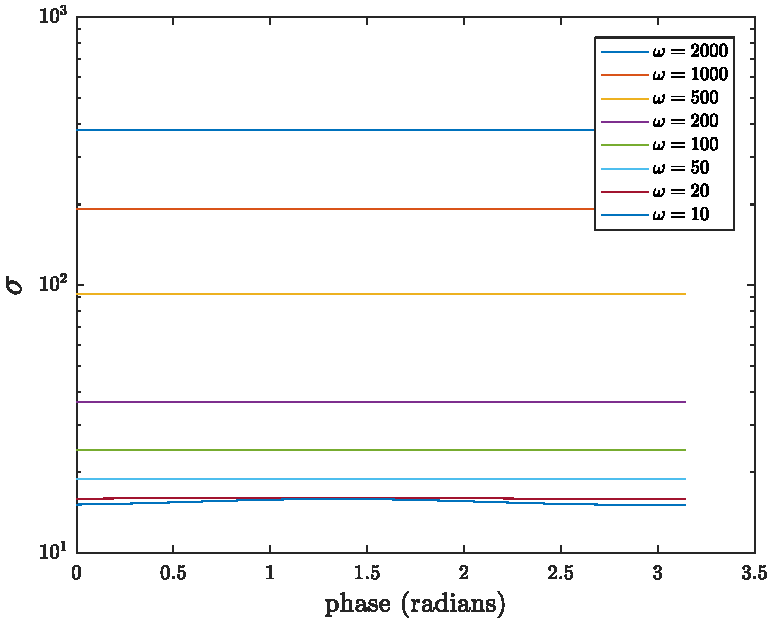
\includegraphics[width=0.5\textwidth]{phase_2D.pdf}
	\caption{Forecast error bars $\sigma^{T+E}$ versus the phase $\phi$. Apart from the smallest frequency $\omega=10$, the error bar remains almost constant. This implies that the sine ($\phi=0$) and cosine ($\phi=\pi/2$) feature models can be constrained independently.}
	\label{forecast_phase_dependence}
\end{figure}

\subsection{$l_{max}$ dependence}

Figure \ref{forecast lmax dependence} shows the graph of forecast error bar $\sigma_{\sin}^{T+E}$ as we increase $l_{max}$. The forecasts were done within angular scale range $2\le l \le l_{max}$, the oscillation frequency $\omega$ set to 100, and assuming 1' beam and 1$\mu K\cdot$arcmin noise. The Planck noise curves were approximated by ones for 5' beam and 47 $\mu K\cdot$arcmin noise for this plot only, since we extend $l_{max}$ to 4000 here. 

The Planck error bar essentially stalls out when $l_{max}$ reaches 2000. The forecast error bar, on the other hand, keeps decreasing until $l_{max}=4000$ thanks to the improved sensitivity in measuring small scales (and large $l$'s). Despite the information loss due to smaller sky coverage $f_{sky}$, the forecast error bar reduces to about 42\% of Planck by $l_{max}=4000$. This corresponds to a factor of 2.4 times improvement to measurement precision on $f_\text{NL}$.

\begin{figure}[ht]
	\centering
	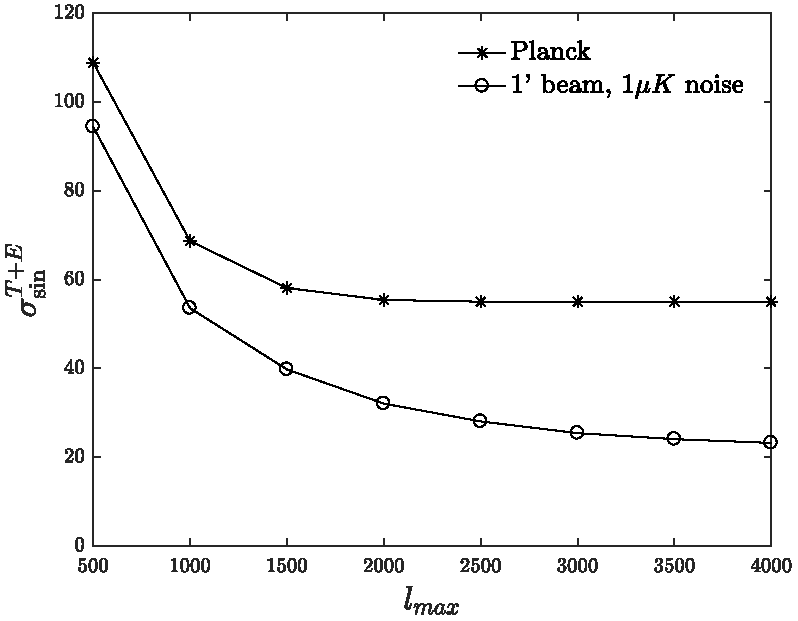
\includegraphics[width=0.5\textwidth]{lmax_dependence.pdf}
	\caption{Forecast error bars $\sigma_{\sin}^{T+E}$ when multipoles $2\le l \le l_{max}$ are included, in comparison with Planck. The oscillation frequency $\omega$ is set to 100 Mpc in all cases. Planck did not have access to the information from modes $l\ge 2000$, but the CMB-S4 experiments are expected to be able to explore modes up to $l=4000$.}
	\label{forecast lmax dependence}
\end{figure}

\subsection{Beam and noise dependence}

Now we explore the effects of different beam width and noise levels on the forecast error bars. Figure \ref{forecast beam and noise dependence} shows forecast $\sigma_{\sin}^{T+E}$ for ranges of beam and noise levels. Their oscillation frequencies are also varied, but only two representatives $\omega=20$ and $2000$ are chosen here. Forecasts for the other values of $\omega$ also display similar dependences on beam width and noise levels.

First of all, note that all estimated error bars in the plot are smaller than Planck, for which $\sigma_{\sin}^{T+E}=34$ when $\omega=20$ and $\sigma_{\sin}^{T+E}=610$ when $\omega=2000$. In fact even the least sensitive CMB-S4 specification of 5' beam and 9$\mu K\cdot$arcmin noise is expected to put better bounds on feature models.

Wider beams and noisier detectors provide less signal and thus larger error bars, as expected. In this range of beam width and noise levels, noise has a bigger effect on the forecast; experiments with 1' beam and 5$\mu K\cdot$arcmin noise yields larger error bars than the ones with 5' beam with 1$\mu K\cdot$arcmin noise. Between the most sensitive specification of 1' beam and 1$\mu K\cdot$arcmin and the least sensitive one with 5' beam and 9$\mu K\cdot$arcmin, $\sigma_{\sin}$ differs by a factor of 1.6.


\begin{figure}[ht]
	\centering
	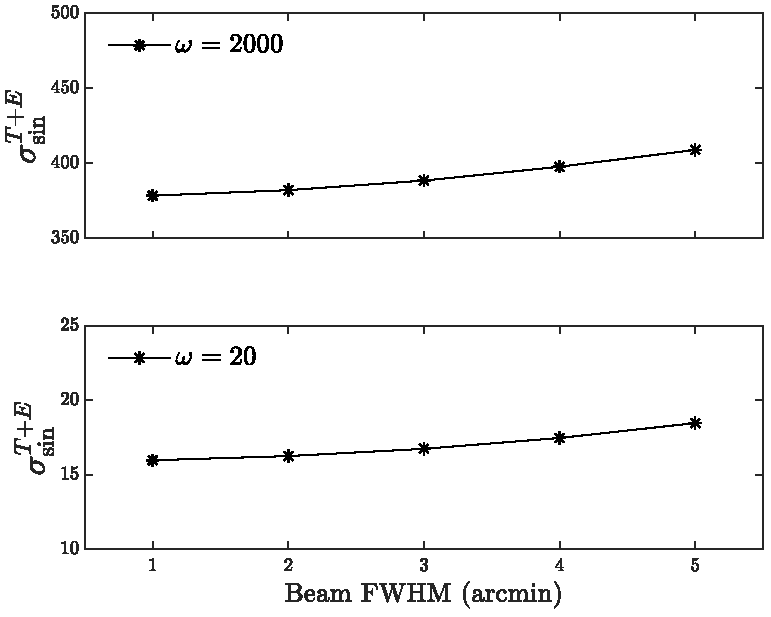
\includegraphics[width=0.45\textwidth]{beam_dependence.pdf}
	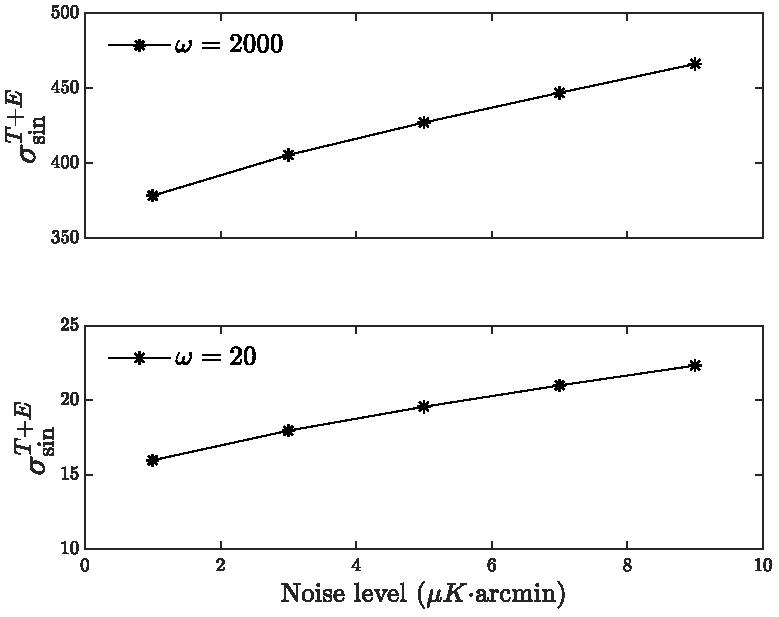
\includegraphics[width=0.45\textwidth]{noise_dependence.pdf}
	\caption{Beam (left) and noise (right) dependences of the forecast error $\sigma_{\sin}^{T+E}$ for $\omega=2000$ (top) and $\omega=20$ (bottom). The noise level was set as 1$\mu K \cdot$arcmin for the first plot, while the second plot had fixed beam FWHM of 1'. We obtain less information from using wider beam and noisier sensors, as expected.}
	\label{forecast beam and noise dependence}
\end{figure}

\subsection{Oscillation frequency dependence}

We present the main results of the forecast. Figure \ref{forecast omega dependence pol} summarises the $\sigma_{\sin}$ forecasts for several different CMB-S4 preliminary specifications, including the Simons Observatory (SO) baseline and goal. Note that the 1/f noise effects are incorporated in SO forecasts but not in other ones. We also provide 1$\sigma$ errors for joint estimators, for which Planck signals from the fraction of the sky not covered by CMB-S4 are combined via $\sigma_\text{joint}^{-2} = \sigma_\text{CMB-S4}^{-2} +  \sigma_\text{Planck}^{-2}$. This method is not statistically optimal but sufficient to give an idea of the joint estimation power.

The most sensitive setup with 1' beam and 1$\mu K \cdot$arcmin noise would yield error bars that are 47-62\% of Planck. These correspond to a factor of 1.6-2.1 improvements. Here relatively smaller improvements are made for high oscillation frequencies. They correspond to smaller momentum scales $k_\ast = 2\pi/3\omega$, or larger angular scales, which benefit less from the increased sensitivity of CMB-S4 experiments. When the results are combined with Planck, the error bar reduces to 45-57\% of Planck, or a factor of 1.7-2.2 improvement.

Forecast error bars from the SO baseline specification and the more ambitious one do not differ very much. Quoting in terms of the baseline values, $\sigma_{\sin}$ lies about 68-86\% of that of Planck or equivalently, 1.2-1.5 times smaller than Planck. Numbers change to 62-74\% when combined with Planck, so that the overall improvement ratio is about 1.3-1.6.

\begin{figure}[ht]
	\centering
	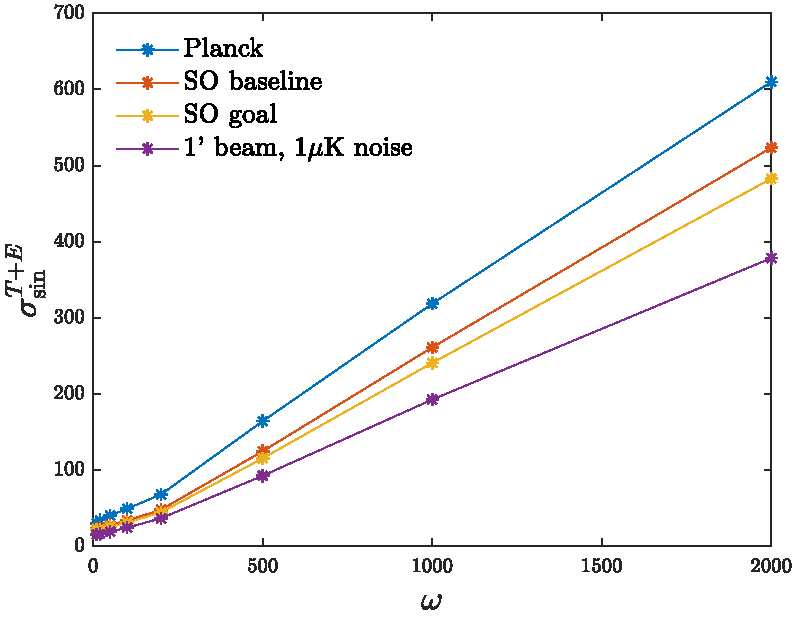
\includegraphics[width=0.45\textwidth]{omega_dependence_pol.pdf}
	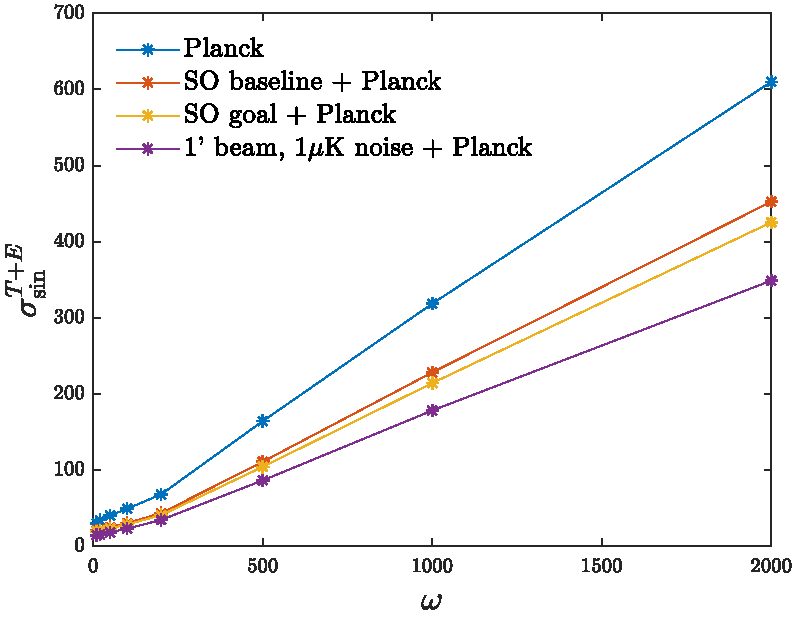
\includegraphics[width=0.45\textwidth]{omega_dependence_combined_pol.pdf}
	\caption{Frequency dependence of the forecast error in comparison to Planck (left). All CMB-S4 specifications would improve constraints on feature models. The most sensitive setup with 1' beam and 1$\mu K \cdot$arcmin noise is expected to yield error bars that are 1.6-2.1 times smaller than Planck. When the Planck results are combined with CMB-S4, we get even stronger constraints (right).}
	\label{forecast omega dependence pol}
\end{figure}

Figure \ref{forecast omega dependence T} shows the results when only the CMB temperature data are used in the forecast. CMB-S4 would in fact be worse than Planck in terms of constraining $f_{NL}^\text{feat}$ for this case. The loss in information due to less sky coverage overwhelms the increased sensitivity. We see again that the real strength of CMB-S4 experiments lies in measuring CMB polarisation.

\begin{figure}[ht]
	\centering
	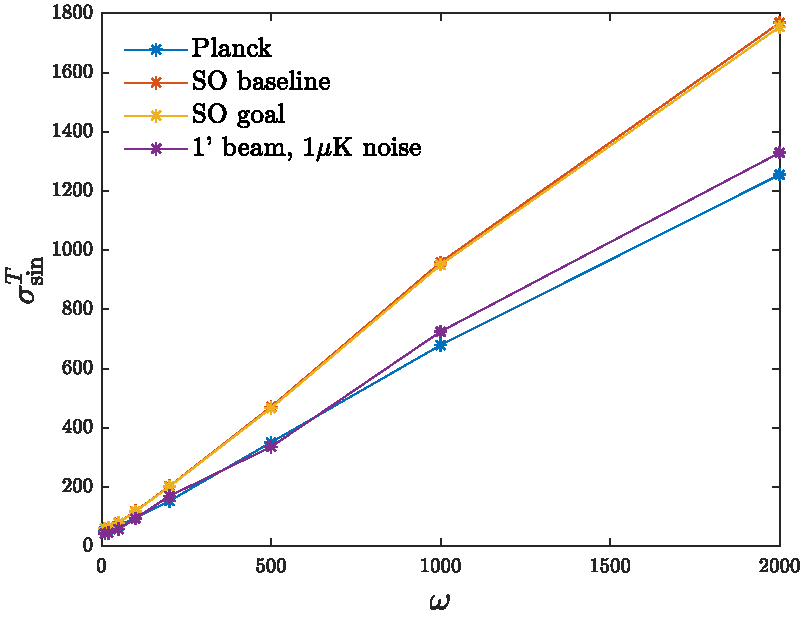
\includegraphics[width=0.45\textwidth]{omega_dependence_T.pdf}
	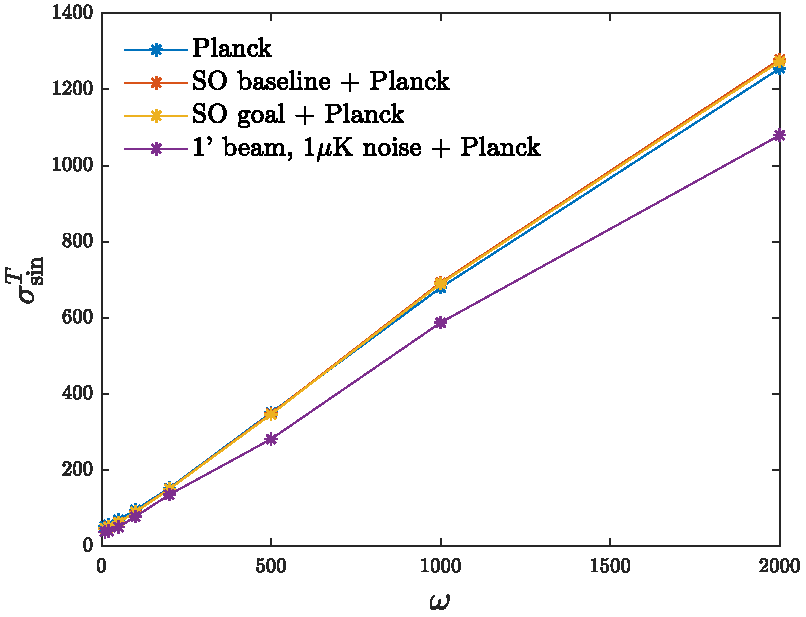
\includegraphics[width=0.45\textwidth]{omega_dependence_combined_T.pdf}
	\caption{Frequency dependence of the forecast error from temperature data only, in comparison to Planck (left). The CMB-S4 experiments would perform worse than Planck when only the temperature map is concerned. After the addition of Planck data the error bars improve only marginally (right). This shows that polarisation data is crucial for constraining feature models.}
	\label{forecast omega dependence T}
\end{figure}

Then how much information do we actually gain from adding E-mode polarisation? Figure \ref{forecast improvement ratio} shows the ratio of $\sigma_{\sin}$s between the temperature-only and polarisation-included analyses. The forecast error bars reduces up to 4.6 times smaller when polarisation information is added, which is much larger than the corresponding Planck value of 2.2. The ratio decreases overall when the joint statistics with Planck are considered. An intriguing feature of this plot is that the ratio is maximised around $\omega=200$ before it starts dropping again.

\begin{figure}[ht]
	\centering
	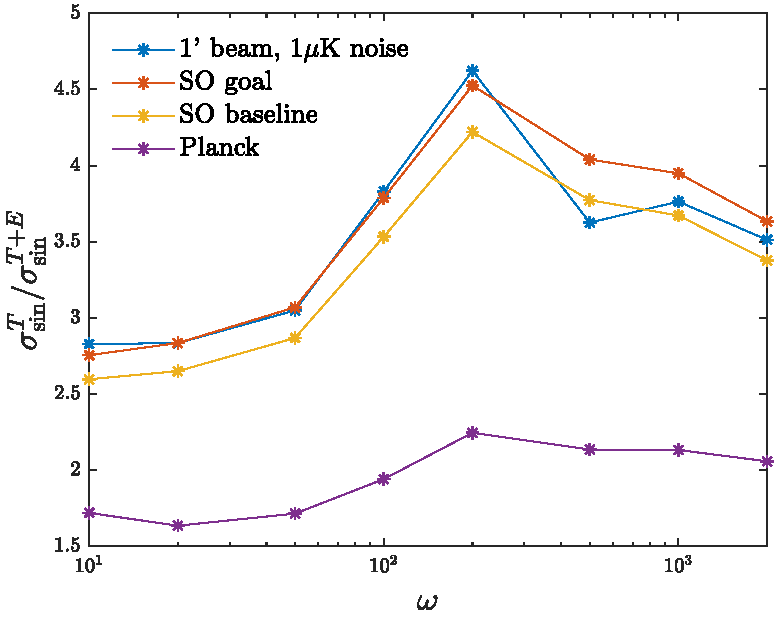
\includegraphics[width=0.45\textwidth]{improvement_ratio.pdf}
	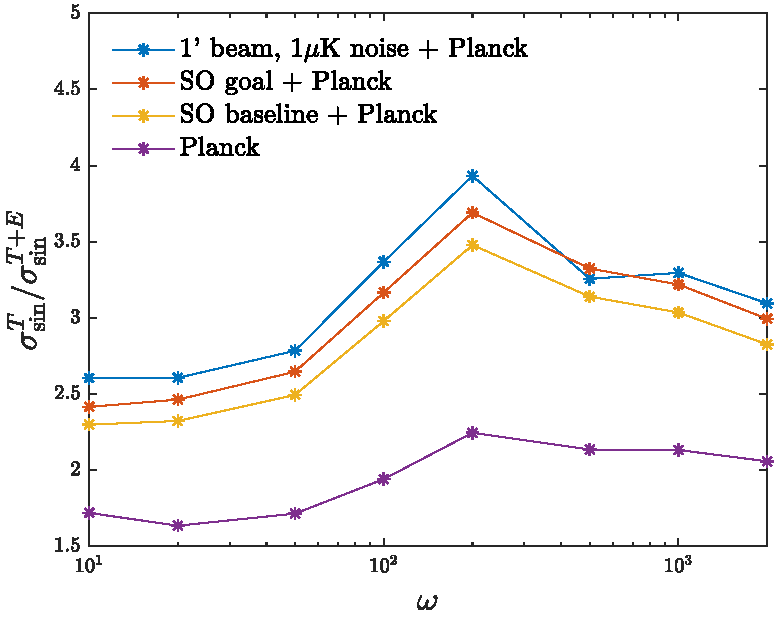
\includegraphics[width=0.45\textwidth]{improvement_ratio_combined.pdf}
	\caption{Improvements on the forecast error when including E-mode polarisation data. Constraints from the CMB-S4 experiments would improve significantly from addition of the polarisation data. The improvement is maximised around $\omega\approx200$ Mpc.}
	\label{forecast improvement ratio}
\end{figure}

In order to gain insight on this behaviour, we performed some simplified computations using the power spectrum. We imposed oscillations on the primordial power spectrum as $P'(k) = P(k)(1+\sin(2\omega k + \phi))$, which is just like our feature model bispectrum template but with $\omega(k_1+k_2+k_3)$ replaced by $\omega(k+k)$. $P'(k)$ is then projected to the late-time harmonic space using the transfer functions;
\begin{equation}
	C_l'^{X_1 X_2} = \frac{2}{\pi} \int k^2 dk P'(k) \Delta_l^{X_1}(k) \Delta_l^{X_2}(k).
	\label{primordial power spectrum to cls}
\end{equation}
We observed that the fractional variation $(C_l'-C_l)/C_l$ displays some oscillations in $l$, and the largest contribution comes from a term $\propto \sin(2\omega l/\Delta\tau)$ where $\Delta\tau$ represents the conformal distance to last scattering surface. This fact can be explained by approximating the transfer function as $\Delta_l(k)\approx (1/3)j_l(k\Delta\tau)$ and noting that the spherical Bessel function has a sharp peak at $l$ for large $l$'s. The integral in (\ref{primordial power spectrum to cls}) therefore picks up a term proportional to $\sin(2\omega l/\Delta\tau)$.

The amplitude of these `maximal' oscillations in $(C_l'-C_l)/C_l$ were then computed using discrete Fourier transform for different values of oscillation scale $\omega$ and two different phases $\phi=0,\pi/2$ (i.e. sine and cosine). The results are shown in Figure \ref{insight feature plot}. Some extra wiggles to the graph come from the phase of oscillations imposed; we indeed see that graphs of sine and cosine oscillate between each other. Some peak features near $\omega\approx70$ and 140 arise from resonances with Baryonic Acoustic Oscillations.

We can think of the computed amplitude as a measure of information $C_l$'s contain about primordial oscillations. First of all, note that the amplitude in all four plots generally decreases as $\omega$ grows. Previously in Figure \ref{forecast omega dependence pol} we saw that the amount of information obtained from the CMB is smaller for larger $\omega$'s, consistent with what can be said from the amplitude analysis. Moreover, the amplitudes for the EE mode are generally larger than the TT mode ones, and their difference is the largest in the $\omega$ range of 70 to 300. This could serve as a heuristic explanation for the improvement in forecast error bars from including polarisation data being maximised around $\omega=200$, as depicted in Figure \ref{forecast improvement ratio}.

\begin{figure}[ht]
	\centering
	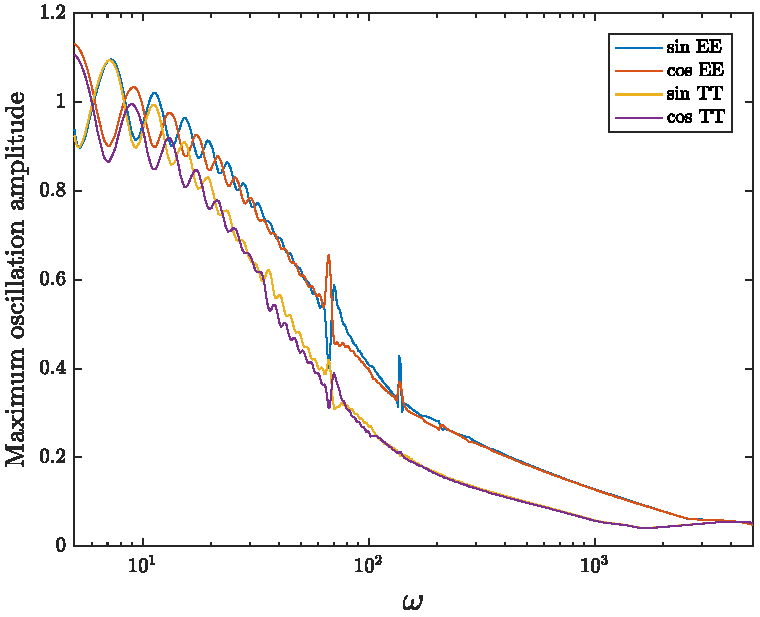
\includegraphics[width=0.7\textwidth]{feature_plot.pdf}
	\caption{The maximum amplitude of oscillations detected in fractional variations of the projected power spectrum $C_l^{TT}$ and $C_l^{EE}$, when extra oscillations $\sin(2\omega k)$ and $\cos(2\omega k)$ were imposed on the primordial power spectrum. Heuristically this shows that E-mode polarisation is more sensitive to the primordial oscillations, especially in the $\omega$ range of 70 to 300. Some peaks near $\omega=70$ and $140$ arise from resonances with Baryonic Acoustic Oscillations. }
	\label{insight feature plot}
\end{figure}


\subsection{Comparison to scale invariant models}

Our pipeline for forecasting $f_{NL}^\text{feat}$ also yields forecasts for $f_{NL}$ of the constant model. Constant models are scale invariant and have trivial shape, so that $B(k_1,k_2,k_3) \propto (k_1 k_2 k_3)^{-2}$.
Forecasts on $f_{NL}^\text{const}$ follow from our pipeline by simply setting the oscillation frequency $\omega = 0$ and phase $\phi = \pi/2$. Table \ref{forecast constant model} summarises the forecast results for several different CMB-S4 specifications mentioned before, using both T and E data and in combination with Planck data from the regions of the sky not covered by CMB-S4. For the 1' beam and 1$\mu K \cdot$arcmin noise setup, the error bar is expected to be reduced by a factor of 2.3 compared to Planck.

\begin{table}[ht]
	\caption{Forecasts on the estimation errors of $f_{NL}$ for the constant model}
	\centering
	\label{forecast constant model}
	\renewcommand{\arraystretch}{1.4}
	\begin{tabular}{ccccc}
		\toprule
		& Planck  & SO baseline + Planck & SO goal + Planck & 1' beam, 1$\mu K$ noise + Planck \\
		\midrule
		$\sigma(f_\text{NL}^\text{const})$ & 23.4 & 14.9 & 14.0 & 10.4 \\
		\bottomrule
	\end{tabular}
\end{table}

The latest Planck constraints on $f_\text{NL}$ of some popular bispectrum templates are given by $f_\text{NL}^\text{local} = 2.5 \pm 5.7$, $f_\text{NL}^\text{equil} = -16 \pm 70$, and $f_\text{NL}^\text{ortho} = -34 \pm 33$ \cite{PlanckCollaboration2015}. CMB-S4 experiments are expected to yield better estimates on these as well. Table \ref{forecast various models} summarises the forecast improvement ratio given in \cite{Abazajian2016} together with the constant and feature model ratios computed in this work.

\begin{table}[ht]
	\caption{Expected improvement ratios of the $f_\text{NL}$ estimation errors for the CMB-S4 1'beam, 1$\mu K$arcmin setup, for various bispectrum templates. The local, equilateral and orthogonal results are quoted from \cite{Abazajian2016}.}
	\centering	
	\label{forecast various models}
	\renewcommand{\arraystretch}{1.4}
	\begin{tabular}{cccccc}
		\toprule
		& Local & Equilateral & Orthogonal & Constant & Feature ($\omega=200$) \\ \midrule
		$\sigma^\text{Planck}/\sigma^\text{CMB-S4}$ & 2.5   & 2.1         & 2.4        & 2.3      & 2.0                \\
		\bottomrule
	\end{tabular}
	
\end{table}

Surprisingly, the estimation error for feature models does not improve as much as other templates. Feature models benefit much more from inclusion of the polarisation data than any other scale independent shapes; for example, $\sigma^{T}/\sigma^{T+E} = 4.6$ for the feature models with $\omega=200$ in CMB-S4 while the value equals 2.8 for the constant models. Because the CMB-S4 experiments would have a significantly enhanced polarisation measurement sensitivity, we originally expected the feature models to be constrained significantly better than Planck.

In order to investigate this lack of improvement, we performed a breakdown analysis on the improvements gained from CMB-S4 temperature and polarisation; we computed $\sigma(f_\text{NL})$ for the constant and feature models using each of the four combinations of Planck / CMB-S4 noise curves for temperature / polarisation (e.g. Planck T + CMB-S4 E). The results are summarised in Table \ref{forecast mixed}.

\begin{table}[ht]
	\caption{Expected improvements on the estimation errors of $f_\text{NL}$ for each combination of Planck / CMB-S4 temperature (T) and polarisation (E) data. Here the CMB-S4 assumes 1' beam and 1$\mu K$arcmin noise. For feature model the oscillation frequency $\omega=200$ and phase $\phi=0$. The sky fraction $f_{sky}=0.4$ for all cases except for Planck T + Planck E, for which $f_{sky}=0.76$.}
	\centering
	\label{forecast mixed}
	\renewcommand{\arraystretch}{1.5}
	\begin{tabular}{c c c c c c c c}
		\toprule
		\multicolumn{2}{c}{$\sigma(f_\text{NL}^\text{const})$}  &  \multicolumn{2}{c}{E}  & \multicolumn{2}{c}{$\sigma(f_\text{NL}^\text{feat})$}  &  \multicolumn{2}{c}{E}  \\
		\cmidrule(lr){3-4} \cmidrule(lr){7-8} 
		\multicolumn{2}{c}{improvements}  & Planck & CMB-S4 & \multicolumn{2}{c}{improvements}  & Planck & CMB-S4 \\
		\cmidrule(lr){1-4} \cmidrule(lr){5-8}
		\multirow{2}{*}{T} & Planck & 1.0 & 1.6 & \multirow{2}{*}{T} & Planck & 1.0 & 1.7 \\
		& CMB-S4 & 1.1 & 2.2 & & CMB-S4 & 0.9 & 1.9 \\
		\bottomrule
	\end{tabular}
\end{table}

% Old table
%\begin{table}[ht]
%	\centering
%	\renewcommand{\arraystretch}{1.4}
%	\parbox{.45\linewidth}{
%		\begin{tabular}{cccc}
%			\multicolumn{2}{c}{\multirow{2}{*}{$\sigma(f_\text{NL}^\text{const})$ improvement}}  &  \multicolumn{2}{c}{E} \\ 
%			\multicolumn{2}{c}{} & Planck & CMB-S4 \\ \hline
%			\multirow{2}{*}{T} & Planck & 1.0 & 1.6 \\
%			& CMB-S4 & 1.1 & 2.2
%		\end{tabular}
%	}
%	\parbox{.45\linewidth}{
%		\begin{tabular}{cccc}
%			\multicolumn{2}{c}{\multirow{2}{*}{$\sigma(f_\text{NL}^\text{feat})$ improvement}} &  \multicolumn{2}{c}{E} \\ 	\multicolumn{2}{c}{} & Planck & CMB-S4 \\ \hline
%			\multirow{2}{*}{T} & Planck & 1.0 & 1.7 \\
%			& CMB-S4 & 0.9 & 1.9
%		\end{tabular}
%	}
%	\caption{Expected improvements on the estimation errors of $f_\text{NL}$ for each combination of Planck / CMB-S4 temperature (T) and polarisation (E) data. Here the CMB-S4 assumes 1' beam and 1$\mu K$arcmin noise. For feature model the oscillation frequency $\omega=200$ and phase $\phi=0$. The sky fraction $f_{sky}=0.4$ for all cases except for Planck T + Planck E, for which $f_{sky}=0.76$.}
%	\label{forecast mixed}
%\end{table}

We see that the constraints on feature models improve by a factor of 1.7 when swapping Planck polarisation noises with the CMB-S4 ones. This factor is indeed larger than the one for constant model, which equals 1.6. The difference is however not significant. It seems that the amount of feature signals in polarisation data left unexplored by Planck is not tremendously large compared to the constant model. The feature model improves less than the constant model when the temperature measurements are enhanced. In fact, for feature models the signal loss from smaller sky fraction $f_{sky}$ eclipses the signal gain from more sensitive temperature measurements. This lack of improvements from temperature causes the full CMB-S4 constraints on the feature model not to improve as much as the constant model overall.

\newpage
\section*{Summary} 

Upcoming CMB Stage-4 experiments will provide an opportunity to measure the CMB temperature anisotropies and polarisation with ever greater precision. The CMB bispectrum estimators for constraining primordial non-Gaussianity would greatly benefit from the improvement in measurement sensitivity. In this research we made forecasts on the $f_\text{NL}$ for feature models, which have not been done so far despite the growing interests on inflation models with oscillations in the primordial spectrum. For efficient forecasts we simplified the bispectrum estimator for $f_\text{NL}$ by orthonormalising the covariance matrix, further optimising the computation. When the most sensitive CMB Stage-4 experiment specification of 1' beam and 1$\mu K$arcmin noise is concerned, we expect a factor of 1.7-2.2 times more stringent constraints compared to Planck. Under the realistic Simons Observatory conditions the improvement would be about 1.3-1.6 to Planck.

Although this is not a massive boost in the estimation power, we can hope to verify the current 4$\sigma$-level signals found in the Planck 2015 analysis. It is also worth noting that the CMB-S4 experiments would allow us to explore the modes with $l>2000$ and localised oscillations on these scales are currently unconstrained. Moreover, though we have only considered linearly-spaced oscillations in this work, we expect even better improvements on the models inducing logarithmically-spaced oscillations where small scale modes with higher $l$ would greatly enhance the constraining power. Lastly, we can expect to cross-validate using these new statistically independent modes to test current constraints further.

We also extensively studied how the forecasts depend on various parameters. Frequency dependences of the ratio between the T and T+E forecasts were particularly illuminating; the improvement from adding polarisation information is maximised around $\omega = 200$. Some simplified calculations were presented to heuristically address this fact. Even though the estimation power on feature models massively benefit from the polarisation data, the expected improvements compared to Planck are quite underwhelming overall. A breakdown analysis on the temperature and polarisation contribution revealed that the feature models would indeed improve more than other scale-independent models if only the polarisation (and not temperature) measurement sensitivity were enhanced to the CMB-S4 standards. However, boosts in the temperature measurements affect scale-independent models more so that they gain more information overall.

The KSW estimator utilises separable bispectrum templates to constrain $f_{NL}$ exactly even for highly oscillatory models, but is inherently restrictive in the range of shapes it can handle. On the other hand, the Modal estimator uses separable basis functions to expand the given bispectrum shape, and thus is able to cover a broad range of non-separable shapes. Due to limitations such as the basis size, however, its accuracy drops for oscillatory models with high frequency. Hence, currently there is a blind spot in the bispectrum analysis for general (non-separable) \textit{and} highly oscillatory models barred off by numerical challenges. We address this in our original research on the high-resolution CMB bispectrum estimator in Chapter \ref{chapter:high_resolution_cmb_bispectrum_estimator}.


%!TEX root = ../thesis.tex
%*******************************************************************************
%****************************** Fifth Chapter **********************************
%*******************************************************************************
\chapter{High-Resolution CMB Bispectrum Estimator} \label{chapter:high_resolution_cmb_bispectrum_estimator}

% **************************** Define Graphics Path **************************
\ifpdf
    \graphicspath{{Chapter5/Figs/Raster/}{Chapter5/Figs/PDF/}{Chapter5/Figs/}}
\else
    \graphicspath{{Chapter5/Figs/Vector/}{Chapter5/Figs/}}
\fi

Despite their major role in constraining a wide range of inflation models, there are only a few implementations of the CMB bispectrum estimator due to computational challenges. The Planck collaboration mainly utilised three independent approaches for their bispectrum analysis \cite{PlanckCollaboration2013,PlanckCollaboration2015,PlanckCollaboration2018}: KSW \cite{Komatsu2005}, Modal \cite{Fergusson2012}, and Binned \cite{Bucher2010}. Standard bispectrum templates for Local, Equilateral and Orthogonal shapes have been constrained using all three methods independently, whilst other more specific ones were covered by only a subset of them.

Some of the most challenging models to handle are those with oscillatory behaviour. Numerous theoretically well-motivated models (\cite{Chen2010foldedResonant,Meerburg2009signatures,Meerburg2010nbd,Meerburg2011cutoff,Hazra2014} and many more, see e.g., \cite{Chen2010review,Chen2016} for reviews) fall into this category. Feature models, as discussed in the previous chapter, often predict linearly spaced oscillations in the bispectrum. Resonance models such as axion monodromy inflation \cite{Silverstein2008monodromy,Flauger2010monodromy} produce log-spaced oscillations modulated with various envelopes. Constraining such models is difficult since oscillations in the bispectra degrade numerical stability of the integrals involved.

Several simple models with oscillations have been studied in the latest Planck analysis using Modal and a few specific KSW-type estimators introduced in \cite{Munchmeyer2014}. Modal estimator covers a wide range of oscillatory models, both with and without envelopes, thanks to the versatility of its mode expansion. It is however difficult to constrain models with high-frequency oscillations using generic mode functions. Modal code allows for choosing a more tailored set of modes for this purpose, but the fact that there are \textit{two} independent sets of mode functions - primordial and late-time - complicates targeted analyses. For each specific selection of mode functions in primordial `$k$' domain, a suitable choice of basis has to be made in late-time `$l$' space. Rapidly oscillating signals may also get lost during the projection from one to the other and cause some numerical issues.

On the other hand, adapted KSW-type estimators \cite{Munchmeyer2014,Munchmeyer2015resonance,Meerburg2016jointResonance} may probe models with much faster oscillations in their bispectra. They exploit separability of specific oscillatory templates and/or Fourier-type bases to obtain accurate constraints in a model-by-model basis. However, these methods are not easily applicable for models with more complicated bispectra, especially the ones that do not depend solely on $K=k_1+k_2+k_3$. The formalism is also specialised to certain types of bispectra and requires a separate implementation for each case. This was one of the main motivations behind the research project; can we have a bispectrum estimator which has the efficiency and versatility of Modal, whilst also benefiting from the precision of the KSW formalism for a more specialised analysis?

We developed a novel CMB bispectrum estimation pipeline CMB-BEst. \footnote{Short for \underline{CMB} \underline{B}ispectrum \underline{Est}imator. The goal of CMB-BEst is to be the best bispectrum estimator with wide applications and great precision.} CMB-BEst has two main strengths over former methods. First of all, it is implemented for completely general basis sets, which allows broad analyses on inflationary models. In fact, the conventional KSW estimator is equivalent to a specific choice of basis in \textit{CMB-BEst}. CMB-BEst can cover any model KSW estimator can, and furthermore, it can simultaneously constrain general bispectrum shapes through primordial mode expansion, just like Modal.

Secondly, CMB-BEst is designed to be able to handle complex and highly oscillatory signals. It does not require a separate set of basis functions for late-time $l$ space, in contrary to Modal. More diverse and specialised choices of basis can therefore be made. The code will be used on numerous inflation models with complex oscillations which are yet to be investigated due to lack of resolution from previous methods. Potential choices of targeted basis for this purpose will be discussed in Section \ref{section:basis_functions}.

Every good thing comes at a price. For CMB-BEst, the price is computational cost. Combining the best of Modal and KSW estimators, CMB-BEst's formalism is more numerically demanding than both of them. Na\"ively speaking, running CMB-BEst for one set of basis functions is equivalent to computing thousands of KSW estimators put together. It is prohibitively expensive unless properly and thoroughly optimised.

We invested a considerable amount of time and effort on optimising the code. Separable mode expansions and subsequent algorithm design were studied in detail for maximal reduction in computational complexity. We also made full use of parallelisation techniques to exploit modern computing architecture. Improving data locality for efficient memory access yielded an order of magnitude speed-up. We illustrate our optimisation procedure in Section \ref{section:implementation}.

The code was then tested thoroughly both internally and against Planck analysis. We used CMB maps and simulations from the Planck satellite experiment and checked that \textit{CMB-BEst} agrees with previous routines map-by-map for various bispectrum templates. Different choices of basis functions within \textit{CMB-BEst} also yielded consistent results. We dedicate Section \ref{section:validation} to presenting the outcome of these consistency checks.

Lastly, we present some applications of the code which serves as a proof of concept. In particular, we connect CMB-BEst to \textsc{Primodal}, an efficient numerical code for computing bispectra of primordial perturbations from a given single field model \cite{Clarke2021}. \textsc{Primodal} uses separable modes for its computation, which enables template-free, direct model-to-constraint analysis when combined with CMB-BEst appropriately. Section \ref{section:proof_of_concept} highlights some results from the combined pipeline. We also identify areas where improvements could be made and discuss directions for future research.

Upcoming surveys will provide major improvements to constraints on primordial non-Gaussianity. Inflationary models with oscillations would also greatly benefit from the enhanced sensitivity, as we discussed in the previous chapter. It is therefore crucial to have a robust and flexible bispectrum estimation routine ready for the future surveys, especially one which can handle high-frequency oscillations. Having another code independent from the existing ones would also be greatly beneficial for cross validation. We expect CMB-BEst to fill this role in the near future.


\section{Formalism}

\subsection{CMB-BEst formalism}
Recall that the optimal CMB bispectrum estimator for a given template can be written as
\begin{align}
	\hat{f}_\text{NL} = \frac{1}{N} \sum_{l_j,m_j} \frac{\mathcal{G}^{l_1 l_2 l_3}_{m_1 m_2 m_3} b_{l_1 l_2 l_3}}{C_{l_1} C_{l_2} C_{l_3}} \left[ a_{l_1 m_1} a_{l_2 m_2} a_{l_3 m_3} - \left( \left< a^G_{l_1 m_1} a^G_{l_2 m_2} \right> a_{l_3 m_3} + \text{2\ cyc.} \right)  \right].		\label{eqn:bispectrum_estimator_standard}
\end{align}
Here we omit superscripts $X$ for temperature and polarisation for notational convenience. Even though the formalism in this section will be presented for CMB temperature data only, the method is general and can easily be extended to include polarisation. For estimation of the full covariance matrix $C_{lm,l'm'}$ needed for the linear term, we use an ensemble average from Gaussian simulations, as denoted by superscripts $G$ and the bracket $\left<\cdot\right>$.

The normalisation factor is given by
\begin{align}
	N = \sum_{l_j} \frac{h_{l_1 l_2 l_3}^2 b_{l_1 l_2 l_3}^2}{C_{l_1} C_{l_2} C_{l_3}}.
\end{align}

The core part of our estimation routine is the separable mode expansion of the shape function;
\begin{align}
	S(k_1, k_2, k_3) := (k_1 k_2 k_3)^2 B(k_1, k_2, k_3) = \sum_{p_j} \alpha_{p_1 p_2 p_3} q_{p_1}(k_1) q_{p_2}(k_2) q_{p_3}(k_3).
\end{align}
Choices for the basis functions $q_p(k)$ are detailed in the next section. Due to the separability, the reduced bispectrum reduces to a compact form of
\begin{align}
	b_{l_1 l_2 l_3} = \sum_{p_j} \alpha_{p_1 p_2 p_3} \int dr \tilde{q}_{p_1}(l_1,r) \tilde{q}_{p_2}(l_2,r) \tilde{q}_{p_3}(l_3,r),
\end{align}
where the \textit{projected} mode functions are defined as
\begin{align}
	\tilde{q}_{p}(l,r) := \frac{2r^\frac{2}{3}}{\pi} \int dk q_p(k) \Delta_l(k) j_l (kr).
\end{align}
Radiative transfer functions $\Delta_l(k)$ and spherical Bessel functions $j_l(kr)$ are denoted the same way as the previous chapter.

Every term appearing in (\ref{eqn:bispectrum_estimator_standard}) except the Gaunt integral is now separable. Using the definition $\mathcal{G}^{l_1 l_2 l_3}_{m_1 m_2 m_3} = \int d^2 \vv{n} Y_{l_1 m_1}(\vv{n}) Y_{l_2 m_2}(\vv{n}) Y_{l_3 m_3}(\vv{n})$, we can render it separable at the cost of introducing an extra integral.

We define the filtered maps as
\begin{align}
	M^{(i)}_p (\vv{n}, r) := \sum_{l,m} \frac{\tilde{q}_p (l,r)}{C_l} a^{(i)}_{lm} Y_{lm} (\vv{n}), \label{def:filtered_maps}
\end{align}
where $a^{(i)}_{lm}$'s are represent the spherical harmonic transform of the $i$th CMB map. For later convenience, we use a convention where $i=0$ corresponds to the observed CMB map. Maps number $1$-$N_\text{sims}$ are Gaussian simulations. Note that without the factors involving $\tilde{q}$ and $C_l$'s, $M$ is simply equal to the original map in real space. Each mode extracts different anisotropy scales present in the map.

The bispectrum estimator (\ref{eqn:bispectrum_estimator_standard}) reduces to
\begin{align}
	\hat{f}_\text{NL}^{(i)} = \frac{1}{N} \sum_{p_j} \alpha_{p_1 p_2 p_3} (\beta^{cub,(i)}_{p_1 p_2 p_3} - 3 \beta^{lin,(i)}_{p_1 p_2 p_3}), \label{eqn:fNL_from_betas}
\end{align}
where most of the computation required is now contained in the `$\beta$'s, given by
\begin{align}
	\beta^{cub,(i)}_{p_1 p_2 p_3} &:= \int dr \int d^2\vv{n} \; M^{(i)}_{p_1} (\vv{n},r) M^{(i)}_{p_2} (\vv{n},r) M^{(i)}_{p_3} (\vv{n},r),	\label{def:beta_cubic} \\
	\beta^{lin,(i)}_{p_1 p_2 p_3} &:= \frac{1}{N_\text{sims}} \sum_{j \neq i} \int dr \int d^2\vv{n} \; M^{(j)}_{p_1} (\vv{n},r) M^{(j)}_{p_2} (\vv{n},r) M^{(i)}_{p_3} (\vv{n},r). \label{def:beta_linear}
\end{align}
Here we evaluate $f_\text{NL}$ estimates for each of the Gaussian simulations $i=1,\cdots,N_\text{sims}$. Naturally, they are normally distributed with mean zero. Under the null hypothesis that the initial fluctuations are purely Gaussian, the value of $f_\text{NL}$ estimated from the observed CMB map is also drawn from the same normal distribution. Any statistically significant deviations from zero would therefore allow us to reject the null hypothesis.

It is important to note that the $\beta$ matrices depend only on the choice of mode functions and input map data, and are independent of the theoretical bispectrum considered. Once $\beta^\text{cub}$ and $\beta^\text{lin}$ are computed and stored, we may constrain any model of interest by decomposing the template to get $\alpha$. The $f_\text{NL}$ estimate is then  a simple dot product: $\vv{\alpha} \cdot \vv{\beta} / N$.

The normalisation can also be obtained in a similar fashion;
\begin{align}
	N = \sum_{p_j, p'_j} \alpha_{p_1 p_2 p_3} \Gamma_{p_1 p_2 p_3, p'_1 p'_2 p'_3} \alpha_{p'_1 p'_2 p'_3}, \label{eqn:normlisation_from_gamma}
\end{align}
or equivalently, $N = \vv{\alpha}^T \Gamma \vv{\alpha}$. We exploit separability once again to compute the $\Gamma$ matrix;
\begin{align}
	\Gamma_{p_1 p_2 p_3, p'_1 p'_2 p'_3} &:= \int dr \int d\mu \mathcal{P}_{p_1 p'_1}(\mu, r, r') \mathcal{P}_{p_3 p'_3}(\mu, r, r') \mathcal{P}_{p_3 p'_3}(\mu, r, r'), 	\label{def:gamma} 	\\
	\mathcal{P}_{p p'}(\mu, r, r') &:= \sum_l \frac{2l+1}{(8\pi)^{1/3} C_l} \tilde{q}_{p'}(l,r) \tilde{q}_p(l,r') P_l(\mu),
\end{align}
where $P_l(\mu)$'s are the Legendre polynomials.

In summary, CMB-BEst computes the main quantities: $\beta^\text{cub}$, $\beta^\text{lin}$, and $\Gamma$. The most computationally expensive part is the linear term $\beta^\text{lin}$ by a couple orders of magnitude in most cases. Considerable effort has been made to optimise the corresponding part of the code, which will be detailed in the following sections.

\subsection{Basis functions} \label{section:basis_functions}

One of the greatest strengths of CMB-BEst lies in its flexibility with the choice of mode functions. We decompose a given shape as a linear combination mode function in three-dimensional space. Hence, we shall refer to them as `basis' functions. Adopting a specialised basis set provides optimised results to specific models of interest, whilst a more general construction of basis allows us to simultaneously constrain a wide range of models.

First, we observe that the KSW estimator \cite{Komatsu2005} is derived from a simple monomial basis in our notation;
\begin{align}
	q_p(k) = k^{p-1}, \;\;\; p = 0, 1, 2, 3.
\end{align}
All three standard templates - local, equilateral, and orthogonal - can be expressed as a sum of separable terms in the form $q_{p_1}(k_1) q_{p_2}(k_2) q_{p_3}(k_3)$. The shape function of the local template, for example, is given by
\begin{align}
	S^{local}(k_1 k_2 k_3) :=& 2A^2 \left[ \frac{k_1^2}{k_2 k_3} + \frac{k_2^2}{k_3 k_1} + \frac{k_3^2}{k_1 k_2}  \right] \\
	=& 2A^2 \left[q_3(k_1)q_0(k_2)q_0(k_3) + q_0(k_1)q_3(k_2)q_0(k_3) + q_0(k_1)q_0(k_2)q_3(k_3) \right],
\end{align}
where $A$ is the primordial power spectrum amplitude. Decomposition coefficients $\alpha_{p_1 p_2 p_3}$ have three non-zero components: $\alpha_{300} = \alpha_{030} = \alpha_{003} = 2A^2$. Coefficients for the equilateral and orthogonal templates can similarly be found.

We set the scalar spectral index as $n_\text{s} = 1$ above for simplicity. In the presence of non-unit $n_\text{s}$, we modify the basis as follows;
\begin{align}
	q_p(k) = k^2 \left[ k_* \left( \frac{k}{k_*} \right)^{(4-n_\text{s})/3} \right]^{p-3}, \;\; p=0,1,2,3. \label{eqn:KSW_basis}
\end{align}
The pivot scale $k_*$ is defined such that the power spectrum evaluates to $A$ at $k=k_*$. Including $k_*$ here ensures that the $q_p(k)$'s have the right units. Note that the prefactor $k^2$ comes from the definition of the shape function and is therefore unaffected by $n_\text{s}$. We will refer to this choice of mode functions to be the `KSW' basis.

For studying models with linearly spaced, high-frequency oscillation, a Fourier-like basis
\begin{align}
	q_0(k) = \sin (\omega k), \; q_1(k) = \cos (\omega k), \label{eqn:Fourier_basis}
\end{align}
for a fixed $\omega$ is an appropriate choice. This is in fact equivalent to the method we used to study feature models in Chapter \ref{chapter:CMB_state-4_forecast}. The small size of the basis lets us efficiently constrain theoretical models with given characteristic scale $\omega$. By scanning over a range of $\omega$, or including modes with different values of $\omega$ in the basis, we may also perform a more comprehensive analysis of oscillatory features.

Lastly, for investigating a wide variety of models simultaneously, we construct large basis sets suitable for decomposing general shape functions. One such example is the following basis which consists of Legendre polynomials;
\begin{align}
	q_p(k) = P_p(\bar{k}), \;\;\text{where}\;\; \bar{k} = \frac{2k-k_\text{min}-k_\text{max}}{k_\text{max}-k_\text{min}}.  \label{eqn:Legendre_basis_no_inv_k}
\end{align}
Here we linearly map the range from $k \in [k_\text{min},k_\text{max}]$ to $\bar{k} \in [-1,1]$, which is the interval where Legendre polynomials are defined. The number of modes are not bounded; the larger the basis, the more complete coverage of theory $k$ space we get.

The Legendre basis functions are inherently orthogonal, so that $\int_{-1}^{1} d\bar{k} P_{l}(\bar{k}) P_{l'}(\bar{k}) = 0$ whenever $l \neq l'$. Orthogonality is essential for this class of basis sets since it allows us to greatly simplify the way of decomposing theoretical templates. We elaborate on the decomposition method in Section \ref{section:primordial_basis_expansion}. 

The Legendre basis also enables direct connection to \textsc{Primodal}, a fast numerical code for computing primordial bispectra from general single-field inflation models \cite{Clarke2021}. \textsc{Primodal} utilises the inherent separability present in the \textit{in-in} formalism to efficiently compute the bispectrum using a separable basis. Using the Legendre polynomials for the basis is optimal for this step, but the methodology is not restricted to any particular choice of basis. The code then outputs the expansion coefficients of the primordial bispectrum with respect to the Legendre polynomials. Hence, the result can be plugged in directly to \textsc{CMB-BEst}, creating one fluid pipeline from the model Lagrangian to $f_\text{NL}$ estimation.

As noted in \cite{Clarke2021}, we may augment the base set of Legendre polynomials with one or more extra functions for better description of some bispectrum templates. One solid choice is to add a mode $q(k) = k^{n_\text{s} -2}$, orthogonalised with respect to the rest of the basis. This significantly boosts the performance of decomposing local-type bispectra.

Ideally, we would like the $k$ range used in the definition (\ref{eqn:Legendre_basis_no_inv_k}) to be as wide as possible so that more information from different scales are incorporated in the estimation process. A wider $k$ range, however, also results in lower resolving power because the interval can fit more oscillations of given frequency. Polynomials of higher degrees are necessary to handle the same bispectra. We found that $k_\text{max}/k_\text{min} = 1000$ is an overall sweet spot for analysing Planck data.

Throughout the rest of this thesis, we refer to a basis with the $k^{n_\text{s} - 2}$ mode and the first 29 Legendre polynomials, totalling 30 modes, defined in the $k$ range with $(k_\text{min}, k_\text{max}) = (2.09 \times 10^{-4}, 2.09 \times 10^{-1})$, as the `Legendre' basis. Any deviation from this set of parameters will be stated explicitly. Note that this is for our convenience during testing only; the code may take any choice of basis.


\subsection{Primordial basis expansion} \label{section:primordial_basis_expansion}

Our formalism assumes that the bispectrum shape of interest can be accurately represented as a linear combination of a chosen basis set; 
\begin{align}
	S(k_1,k_2,k_3) = \sum_{p_j} \alpha_{p_1,p_2,p_3} \; Q_{p_1 p_2 p_3}(k_1, k_2, k_3),
\end{align}
where the three-dimensional mode functions are defined as
\begin{align}
	Q_{p_1 p_2 p_3} (k_1, k_2, k_3) := q_{p_1}(k_1) \; q_{p_2}(k_2) \; q_{p_3}(k_3).
\end{align}
For some models the coefficients $\alpha_{p_1 p_2 p_3}$ are obtained analytically. The local shape function with respect to the KSW basis is a simple example; $\alpha_{300}=\alpha_{030}=\alpha_{003}=2A^2$ and zero otherwise. For other models, the shape function needs to be expanded with respect to the chosen basis. 

Shape functions are defined on the same domain as bispectra: $(k_1,k_2,k_3) \in \mathbb{R}^3$ where $k_1$, $k_2$, and $k_3$ form a triangle. We cannot observe scales smaller than a certain size in practice, which places an upper bound on $k$: $k < k_\text{max}$. The resulting domain in three dimensions is shown in Figure \ref{fig:tetrapyd}.

\begin{figure}[htbp!] 
	\centering    
	\hspace{10pt}
	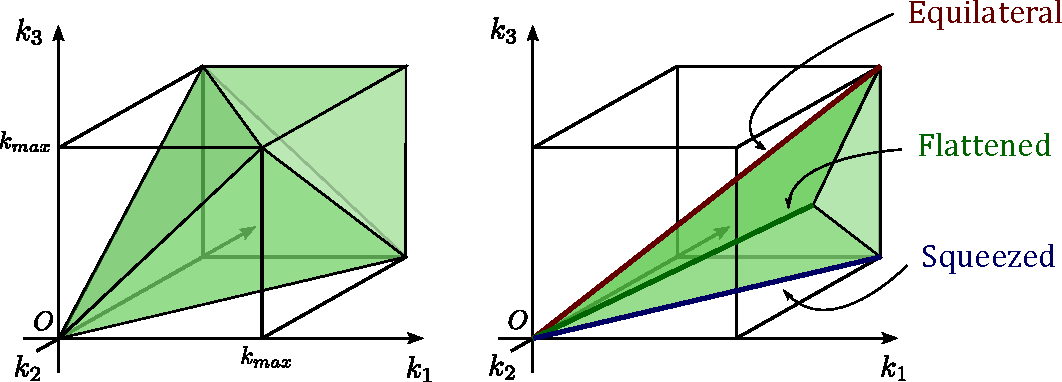
\includegraphics[width=1.0\textwidth]{tetrapyd.pdf}
	\caption{Tetrapyd domain in which the shape functions are defined. Left: the full region specified by triangle inequalities and an upper bound $k_\text{max}$. Right: one sixth slice of the tetrapyd from which shape functions are uniquely determined by symmetry in the $k$'s. Edges representing the equilateral, flattened and squeezed configurations are annotated.}
	\label{fig:tetrapyd}
\end{figure}

We follow \cite{Fergusson2010general} and denote this domain consisting of two tetrahedrons glued together as the `tetrapyd'. Note that all shape functions of interest are symmetric in the $k$'s, so we may restrict our interest to a region where $k_1 \ge k_2 \ge k_3$ (right of Figure \ref{fig:tetrapyd}). We dub the resulting tetrahedron with one sixth the original volume the `sliced' tetrapyd, somewhat unoriginally. The three main types of triangle configurations correspond to three edges of the sliced tetrapyd: equilateral ($k_1=k_2=k_3$), flattened ($k_1 = k_2 + k_3$), and squeezed ($k_1 = k_2 \gg k_3$). \footnote{To be precise, the edges for flattened represent $k_1/2 = k_2 = k_3$, and the squeezed one is defined as $k_1=k_2$, $k_3=0$. The edges by themselves are unphysical, but points near these lines correspond to the limits described.} Figure \ref{fig:Legendre_basis_functions_3D} shows some of the Legendre basis functions plotted in three dimensions.

\begin{figure}
	\centering    
	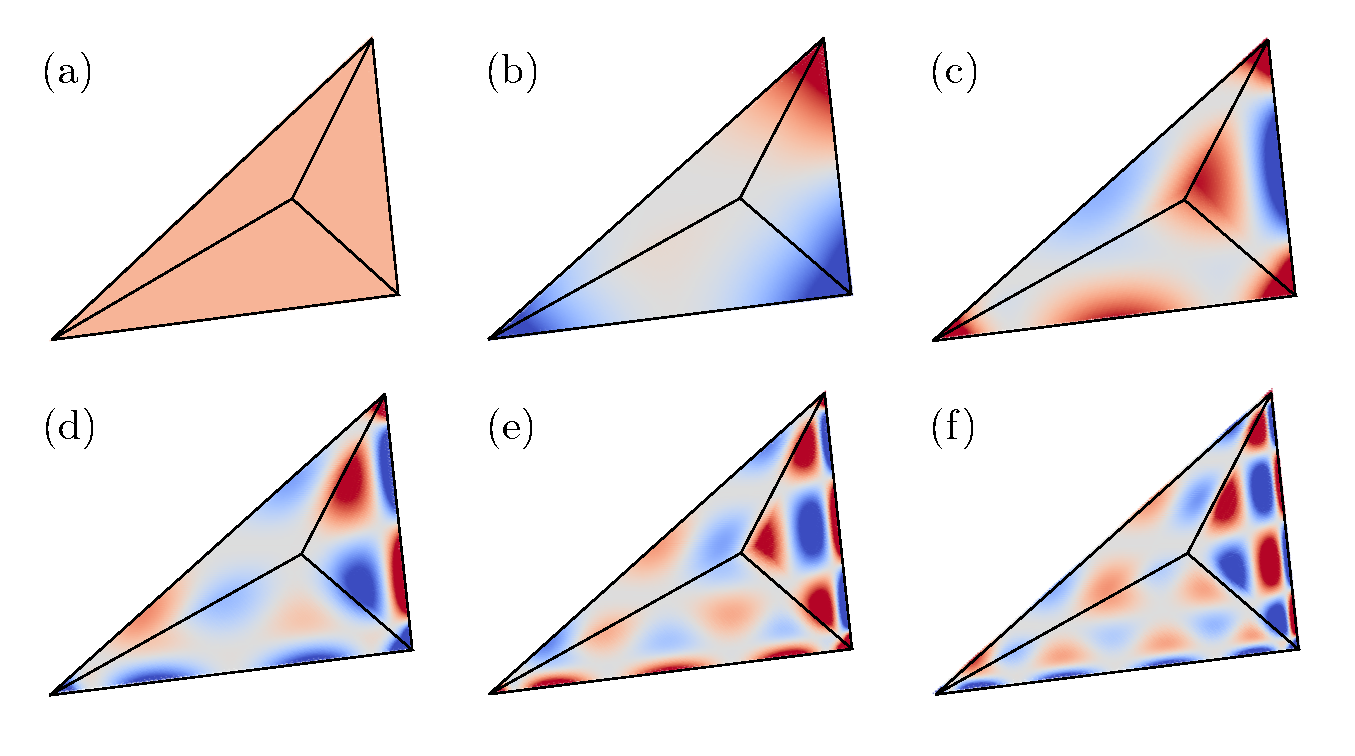
\includegraphics[width=1.0\textwidth]{legendre_modes_3D_final.pdf}
	\caption{Examples of our Legendre basis functions, evaluated on the sliced tetrapyd domain shown in Figure \ref{fig:tetrapyd}. Functions are defined as $Q_{p_1 p_2 p_3}(k_1,k_2,k_3) := P_{p_1}(k_1) P_{p_2}(k_2) P_{p_3}(k_3)$, where $P_l(k)$ are Legendre polynomials. Here we plot $p_1 = p_2 = p_3 = p$, where $p$ equals (a) $0$, (b) $1$, (c) $2$, (d) $3$, (e) $4$, and (f) $5$. A single colour map is used across the plots: red and blue correspond to $+1$ and $-1$, respectively.}	
	\label{fig:Legendre_basis_functions_3D}
\end{figure}

Let $V_{\vv{k}}$ be the subset of $\mathbb{R}^3$ representing the sliced tetrapyd. By choosing a natural inner product
\begin{align}
	\left< S_1, S_2 \right> = \int_{V_{\vv{k}}} d^3\vv{k} \;\; S_1(\vv{k}) S_2(\vv{k}), \label{eqn:tetrapyd_inner_product}
\end{align}
we restrict our attention to an $L^2$ space defined on $V_{\vv{k}}$: a vector space consisting of square-integrable functions.
\footnote{Note that the local shape function $S(k_1,k_2,k_3) = (k_1^2 / k_2 k_3 + \text{2 cyc.})$ is not in fact square-integrable due to its divergence as $k_i \rightarrow 0$. We work around this problem by prescribing a lower bound $k \ge k_\text{min}$, which is also the case in numerical calculations.}
A set of three-dimensional basis functions $Q_{\vv{p}}$ with size $N$ spans a subspace $U_{Q} \subset L^2(V_{\vv{k}})$ of dimension at most $N$.

Using this notation, expanding a given shape function $S$ with respect to a basis set $Q$ is equivalent to finding its orthogonal projection into $U_{Q}$;
\begin{align}
	&S = S^{\parallel} + S^{\perp}, \;\;\;\text{where} \\
	&S^{\parallel} \in U_Q \;\;\;\;\text{and} \;\;\; \left< S^{\perp}, Q' \right> = 0, \; \forall Q' \in U_Q.
\end{align}
As long as $\left\| S^\perp \right\| \ll \left\| S \right\|$, we may approximate
\begin{align}
	S \approx S^\parallel = \sum_{\vv{p}} \alpha_{\vv{p}} Q_{\vv{p}}.  \label{eqn:primordial_basis_projection}
\end{align}
The decomposition coefficients $\alpha$ are obtained by taking inner product with $Q_{\vv{p}}$ on both sides.
\begin{align}
	\left< S, Q_\vv{p} \right> = \left< Q_\vv{p}, Q_{\vv{p}'} \right> \alpha_{\vv{p}'}. \label{eqn:primordial_basis_expansion_SQ_and_QQ}
\end{align}
From above, we can compute $\alpha_\vv{p}$ by inverting the matrix $\Gamma_{\vv{p} \vv{p}'} = \left< Q_\vv{p}, Q_{\vv{p}'} \right>$. Alternatively, orthonormalising the basis with respect to the inner product $\left< , \right>$ turns $\Gamma$ to an identity matrix, trivialising the inversion process.

We rewrote the formalism using linear analysis language here to emphasize two aspects of our primordial basis expansion. First, even though we chose a simple inner product (\ref{eqn:tetrapyd_inner_product}) for now, the method is completely general and we may freely choose a different inner product. For example, non-unit weights $w(\vv{k})$ can be included in the integrand and/or the domain of integration may be changed. Doing so alters how we decompose shape functions in terms of our basis.

Second, we highlight the fact that basis expansion is in essence a minimisation problem with respect to chosen inner product, which is often oblivious of late-time physics. The orthogonal projection of $S$ to subspace $U_Q$ is a point in $U_Q$ which has minimal distance to $S$: $\left\| S - S^\parallel \right\|$ is minimised. The obtained $S^\parallel$, however, is not necessarily the best description of $S$ when we consider their late-time counterparts in $l$ space. Some errors with small norm $\left\| \Delta S \right\|$ might get enhanced when convolved with transfer functions, yielding large reduced bispectrum $\Delta b_{l_1 l_2 l_3}$. Meanwhile, sometimes large differences in $S$ are completely unobservable late-time and provide mostly identical constraints on $f_\text{NL}$.

With these points in mind, we define the following metrics to compare shape functions in primordial space;
\begin{align}
	\text{Corr}(S_1, S_2) &:= \frac{\left< S_1, S_2 \right>}{ \sqrt{ \left< S_1, S_1 \right> \left< S_2, S_2 \right> } }, \\
	\epsilon^2(S_1, S_2) &:= \frac{\left< S_1 - S_2, S_1 - S_2 \right> }{\sqrt{\left< S_1, S_1 \right> \left< S_2, S_2 \right>}}. \label{def:primordial_shape_epsilon}
\end{align}
Corr$(S_1,S_2)$ measures correlation between the two shapes and is independent of the normalisation. $\epsilon(S_1,S_2)$ is the distance between the two shapes, which reduces to $\sqrt{2 - 2\;\text{Corr}(S_1,S_2)}$ when $S_1$ and $S_2$ have equal amplitude. We use both of these values to test if our primordial basis expansion has converged to the target shape function. 

Inverting the matrix $\Gamma_{\vv{p} \vv{p}'} = \left< Q_\vv{p}, Q_{\vv{p}'} \right>$ in \eqref{eqn:primordial_basis_expansion_SQ_and_QQ} can be tricky in practice. The $p_\text{max}^3 \times p_\text{max}^3$ matrix is not only large in size for high $p_\text{max}$, but also near singular. Some of the three-dimensional mode functions $Q_\vv{p}$ become linearly dependent within tetrapyd even if they are constructed from independent modes in one dimension. Presence of such degenerate modes introduces severe numerical instability during inversion.

For our Legendre basis, we use a small trick to get around this problem. Motivated by the fact that Legendre polynomials form an orthogonal basis in one dimension, we extend the domain of integral in the inner product \eqref{eqn:tetrapyd_inner_product} to a cube containing the tetrapyd instead. Most template shape functions have an analytic form and can easily be extended in this region. As long as $\int dk \; q_p(k) q_{p'}(k) = \delta_{pp'}$, the decomposed coefficients for a given $S$ can be found by
\begin{align}
	\alpha^{(t)}_{p_1 p_2 p_3} = \int dk_1 \int dk_2 \int dk_3 \; S^{(t)}(k_1, k_2, k_3) q_{p_1}(k_1) q_{p_2}(k_2) q_{p_3}(k_3). \label{eqn:basis_expansion}
\end{align}
Note that the three-dimensional integral can now be split into three separate one-dimensional integrals in range $[k_\text{min}, k_\text{max}]$. By performing the three integrals one by one, we obtain a numerically stable algorithm that is fast and memory efficient. Decomposing a shape evaluated on $1000^3$ $k$ grid points with respect to $30^3$ Legendre basis functions only takes a few seconds in our \textsc{C} code.

After we obtain coefficients from (\ref{eqn:basis_expansion}), we evaluate the accuracy of the expansion using the inner product defined in tetrapyd because it is the only physical region where our shape function matters. Since the cube includes tetrapyd, good convergence in the cube guarantees a small error within the tetrapyd in most cases. The only exception is when the target shape function blows up outside the tetrapyd. We will see such examples in later sections.


\section{Implementation and optimisation} \label{section:implementation}

CMB bispectrum estimation is a numerically challenging task. All existing approaches exploit the separability of multi-dimensional integrals to reduce computational complexity, because it is practically impossible otherwise. Planck analysis provided constraints to primordial non-Gaussianity from various bispectrum templates, but having limited computing resources was what stopped us from exploring further. Numerous shapes such as complex oscillatory models have been outside our reach, despite being theoretically well-motivated.

The CMB-BEst formalism significantly reduces the amount of computation needed for CMB bispectrum estimation. Obtaining the linear term $\beta^\text{lin}$ in (\ref{def:beta_linear}), however, is still prohibitively expensive unless thoroughly optimised. Performance is especially crucial here since it directly affects the breadth of models we can cover; the faster the code, the higher number of modes we can have, and so the more shapes we can expand in our basis accurately.

In this section, we provide details for various aspects of our optimisation process: algorithm design, parallel computing, and data locality improvements. Final specifications and data files used are outlined at the end.

Throughout this section we will treat the functions of interest as discrete arrays. Our notation for indices and their limits are summarised in Table \ref{table:index_conventions}. We adopt a simple trapezoidal rule for most numerical integrals. For the $\mu$ integral in (\ref{def:gamma}), however, we use Gauss-Legendre quadrature computed from the public code \textsc{Quadpts} \cite{Hale2013} due to the highly oscillatory and unstable nature of the integral. Multi-dimensional arrays are stored in the row major order following the \textsc{C} convention for efficiency. We use the \textsc{Healpix} library \cite{Gorski2005healpix} for pixelisation of the sky, which includes the \textsc{Libsharp} \cite{Reinecke2013libsharp} library for Spherical Harmonic Transforms (SHTs).

\begin{table}[htbp]
	\caption{Our index conventions for discretised arrays and their sizes.}
	\centering
	\label{table:index_conventions}
	\renewcommand{\arraystretch}{1.5} 
	\begin{tabular}{m{0.1\textwidth}  m{0.1\textwidth}  m{0.7\textwidth}} \toprule
		Index & Range & Description \\
		
		\midrule
		$r$ & $[0, N_r)$ & Line-of-sight integral $r$ grid index. \\
		
		$p, p_j$ & $[0, p_\text{max})$ & Mode number. $p_j$ is a shorthand for $(p_1, p_2, p_3)$. \\
		
		$i,j$ & $[0, N_\text{sims}]$ & Map number. Index $i=0$ corresponds to the observed CMB map, while $i>0$ are for simulated Gaussian maps. \\			
		
		$n$ & $[0, N_\text{pix})$ & Map pixel number. \\ 
		
		$l,m$ & $[0, l_\text{max})$ & Spherical harmonic multipole moments. Note $-l \le m \le l$. \\
		
		$\mu$ & $[0, N_\mu)$ & Gauss-Legendre quadrature $\mu$ grid index. \\
		
		\bottomrule
	\end{tabular}
\end{table}

\subsection{Algorithm}

Our goal is to compute three key quantities: $\Gamma$ (\ref{def:gamma}), $\beta^\text{cub}$ (\ref{def:beta_cubic}), and $\beta^\text{lin}$ (\ref{def:beta_linear}). The matrix $\Gamma$ allows us to find the normalisation factor $N$ for a given theoretical template, while the two $\beta$'s provide the amplitude of $f_\text{NL}$ for each of the CMB maps and simulations used up to normalisation.

In most cases of interest, the bottleneck point of our pipeline is computing the linear term $\beta^\text{lin}$. Even though the $\Gamma$ matrix computation through (\ref{def:gamma}) grows more rapidly with the number of basis functions ($\propto p_\text{max}^6$) than the $\beta$'s ($\propto p_\text{max}^3$), it does not involve operations with high-definition maps and remains subdominant in terms of total cost.

We dedicate this section to explain our algorithm design for $\beta$ computation in detail. The discretised versions of (\ref{def:beta_cubic}-\ref{def:beta_linear}) are given by
\begin{align}
	\beta^\text{cub}(i, p_1,p_2,p_3) &= \sum_r \sum_n \; M(r, i, p_1, n) \cdot M(r, i, p_2, n) \cdot M(r, i, p_3, n), \\
	\beta^\text{lin}(i, p_1,p_2,p_3) &= \sum_r \sum_{j \neq i} \sum_n \; M(r, j, p_1, n) \cdot M(r, j, p_2, n) \cdot M(r, i, p_3, n).
\end{align}
The order of indices are chosen such that later calculations have optimal memory layouts. Some integral weights and factors are absorbed into arrays for brevity.

Note that the data arrays for different values of $r$ are completely independent from each other. This provides us with a natural way to distribute tasks. We compute and save contributions to $\beta$'s for each $r$ separately. The summation over $r$ is performed at the end. Therefore, throughout the rest of this chapter, we assume that $r$ is fixed and drop the $r$ dependence in the descriptions of our algorithms.

The filtered map arrays $M(i,p,n)$ are obtained as follows. A given map $i$ is first transformed into spherical harmonic coefficients $a^{(i)}(l,m)$s via SHT. We then compute $\tilde{q}_(p,l) * a(i,l,m) / C(l)$ from (\ref{def:filtered_maps}), which is fed into reverse SHT to synthesise the filtered maps.

As a rough guide to the size of each summation, we typically have $N_{sim} \approx 150$ simulations, $p_\text{max} = 30$ modes, and $N_\text{pix} = 50,331,648$ pixels. \footnote{This value corresponds to $N_{side} = 2048$ in Healpix. $N_\text{pix} = 12 N_{side}^2$} Considering the fact that one double-precision array of size $\sim 50$ million pixels takes about 400MB of memory space, this is indeed a task for supercomputers.

Our first and most straightforward method of computing $\beta$s is outlined in Algorithm \ref{alg:beta_first_attempt}. Computational complexity of each innermost loop is annotated on the right hand side.

\begin{algorithm}[htbp]
	\caption{Computing $\beta$s: the na\"ive method}
	\label{alg:beta_first_attempt}
	\begin{algorithmic}[1] % The number tells where the line numbering should start	
		\State Allocate $M(i,p,n)$
		\Comment{Memory $\sim N_\text{sims} \cdot p_\text{max} \cdot N_\text{pix}$}

		\\
		\For{each map $i$}
			\For{each mode $p$}
			\Comment{$O(N_\text{sims} \cdot p_\text{max} \cdot N_\text{pix}^{3/2})$}
				\State \textbf{compute} $M(i,p,n)$ by SHT
			\EndFor
		\EndFor \Comment{$M(i,p,n)$ ready}
		\\
		
		\For{each map $i$}
			\For{each set of modes $(p_1,p_2,p_3)$}
				\For{each pixel $n$}
				\Comment{$O(N_\text{sims} \cdot p_\text{max}^3 \cdot N_\text{pix})$}
					\State $\beta^\text{cub}(i, p_1, p_2, p_3) \pluseq M(i,p_1,n) \cdot M(i,p_2,n) \cdot M(i,p_3,n)$
				\EndFor
			\EndFor
		\EndFor

		\\	
		\For{each map $i$}
			\For{each map $j \neq i$}
				\For{each set of modes $(p_1,p_2,p_3)$}
					\For{each pixel $n$}
					\Comment{$O(N_\text{sims}^2 \cdot p_\text{max}^3 \cdot N_\text{pix})$}
						\State $\beta^\text{lin}(i, p_1, p_2, p_3) \pluseq M(j,p_1,n) \cdot M(j,p_2,n) \cdot M(i,p_3,n)$
					\EndFor
				\EndFor
			\EndFor
		\EndFor

	\end{algorithmic}
\end{algorithm}

Here, we first obtain the filtered maps $M(i,p,n)$ via SHT for each map and modes. The full results are stored in memory. Next, we iterate through each map and set of modes $(p_1, p_2, p_3)$ and sum over each of the map pixels to obtain $\beta^\text{cub}$ and $\beta^\text{lin}$. Symmetries in the indices are respected; we only loop over $(p_1,p_2,p_3)$ satisfying $p_1\ge p_2$ for the linear terms, and $p_1\ge p_2\ge p_3$ for the cubic ones.

SHT typically scales as $\propto l_\text{max}^3$, where $l_\text{max}$ is the maximum degree of spherical harmonic functions used. The total number of pixels $N_\text{pix}$ grows $\propto l_\text{max}^2$ when chosen appropriately for resolution, hence the SHT costs $O(N_\text{sims}\cdot p_\text{max} \cdot N_\text{pix}^{3/2})$. The most expensive part of this algorithm is still the loop where we calculate the linear term, which scales as $O(N_\text{sims}^2 \cdot p_\text{max}^3 \cdot N_\text{pix})$.

Our first major optimisation comes from the observation that we may swap the order of summations to reduce the computation. By precomputing $C(p_1, p_2, n) = \sum_j M(j,p_1,n) \cdot M(j,p_2,n)$, we require one fewer loop over maps for $\beta^\text{lin}$, leading to a factor of $N_\text{sims}\sim150$ improvement. Algorithm \ref{alg:beta_second_attempt} shows a pseudocode for this method.

\begin{algorithm}[htbp]
	\caption{Computing $\beta$s: optimised for computation}
	\label{alg:beta_second_attempt}
	\begin{algorithmic}[1] % The number tells where the line numbering should start	
		\State Allocate $M(i,p,n)$ \Comment{Memory $\sim N_\text{sims} \cdot p_\text{max} \cdot N_\text{pix}$}
		\State Allocate $C(p_1,p_2,n)$ \Comment{Memory $\sim p_\text{max}^2 \cdot N_\text{pix}$}
		\\
		\For{each map $i$}
			\For{each mode $p$}
				\Comment{$O(N_\text{sims} \cdot p_\text{max} \cdot N_\text{pix}^{3/2})$}
				\State \textbf{compute} $M(i,p,n)$ by SHT
			\EndFor
		\EndFor \Comment{$M(i,p,n)$ ready}
		\\
		\For{each map $j$}
			\For{each pair of modes $(p_1,p_2)$}
				\For{each pixel $n$}
					\Comment{$O(N_\text{sims} \cdot p_\text{max}^2 \cdot N_\text{pix})$}
					\State $C(p_1,p_2,n) \pluseq M(j,p_1,n) \cdot M(j,p_2,n)$
				\EndFor
			\EndFor
		\EndFor \Comment{$C(p_1,p_2,n)$ ready}
		\\
		\For{each map $i$}
			\For{each set of modes $(p_1,p_2,p_3)$}
				\For{each pixel $n$}
					\Comment{$O(N_\text{sims} \cdot p_\text{max}^3 \cdot N_\text{pix})$}
					\State $\beta^\text{cub}(i, p_1, p_2, p_3) \pluseq M(i, p_1, n) \cdot M(i, p_2, n) \cdot M(i, p_3, n)$
					\State $\beta^\text{lin}(i, p_1, p_2, p_3) \pluseq C(p_1, p_2, n) \cdot M(i, p_3, n)$
				\EndFor
			\EndFor
		\EndFor
	\end{algorithmic}
\end{algorithm}

Note that the resulting sum fo $\beta^\text{lin}$ includes an unwanted contribution from the case where $j=i$, since $C(p_1,p_2,n)$ is obtained by summing over all maps. Thankfully, this extra contribution is exactly equal to the cubic term. We just have to subtract $\beta^\text{cub}$ from the total sum to get the correct value of $\beta^\text{lin}$.

We shaved off a whole loop at the cost of extra memory usage. For our purposes $N_\text{sims} \sim 150 > p_\text{max} = 30$, so the additional space required for $C(p_1,p_2,n)$ is relatively small compared to $M(i,p,n)$. The symmetry in $p_1$ and $p_2$ also means that we only need to store $p_\text{max}(p_\text{max}+1)/2$ maps instead of $p_\text{max}^2$ for $C$.

Our next challenge is the amount of memory required to save $M(i,p,n)$. For the parameters mentioned above, this is $\approx 1.8$TB, which is quite significant. Although it is not impossible to find supercomputing systems which can accommodate such large arrays, reducing the memory usage would be highly beneficial. We seek to achieve this whilst keeping the overall computational complexity to be $O(N_\text{sims} \cdot p_\text{max}^3 \cdot N_\text{pix})$ as before.

We observe that most summations are done for a single map $i$. The array $C(p_1,p_2,n)$ is required to be computed before the main loop for $\beta^\text{lin}$, but otherwise there are no `mixing' between the maps. We exploited this fact to develop Algorithm \ref{alg:beta_third_attempt}.

\begin{algorithm}[htbp]
	\caption{Computing $\beta$s: fast and memory efficient}
	\label{alg:beta_third_attempt}
	\begin{algorithmic}[1] % The number tells where the line numbering should start	
		\State Allocate $m(p,n)$ \Comment{Memory $\sim p_\text{max} \cdot N_\text{pix}$}
		\State Allocate $C(p_1,p_2,n)$ \Comment{Memory $\sim p_\text{max}^2 \cdot N_\text{pix}$}
		\\
		\For{each map $i$}
			\For{each mode $p$}
				\Comment{$O(N_\text{sims} \cdot p_\text{max} \cdot N_\text{pix}^{3/2})$}
				\State \textbf{compute} $M(i,p,n)$ by SHT and store in $m(p,n)$
			\EndFor
			\\
			\For{each pair of modes $(p_1,p_2)$}
				\For{each pixel $n$}
				\Comment{$O(N_\text{sims} \cdot p_\text{max}^2 \cdot N_\text{pix})$}
					\State $C(p_1,p_2,n) \pluseq m(p_1,n) \cdot m(p_2,n)$
				\EndFor
			\EndFor
		\EndFor
		\Comment{$C(p_1,p_2,n)$ ready}
		\\
		\For{each map $i$}
			\For{each of mode $p$}
				\Comment{$O(N_\text{sims} \cdot p_\text{max} \cdot N_\text{pix}^{3/2})$}
				\State \textbf{compute} $M(i,p,n)$ by SHT and store in $m(p,n)$
			\EndFor
			\\
			\For{each set of modes $(p_1,p_2,p_3)$}		\label{alg:thrid_attempt_main_loop}	
				\For{each pixel $n$}
					\Comment{$O(N_\text{sims} \cdot p_\text{max}^3 \cdot N_\text{pix})$}	
					\State $\beta^\text{cub}(i, p_1, p_2, p_3) \pluseq m(p_1,n) \cdot m(p_2,n) \cdot m(p_3,n)$
					\State $\beta^\text{lin}(i, p_1, p_2, p_3) \pluseq C(p_1, p_2, n) \cdot m( p_3, n)$
				\EndFor
			\EndFor
		\EndFor
	\end{algorithmic}
\end{algorithm}

Algorithm \ref{alg:beta_third_attempt} dramatically reduces the amount of memory required, at the cost of doubling the SHTs for computing $M(i,p,n)$s. The first time through, SHT results from each map are used to find $C(p_1,p_2,n)$. After a full loop over maps we have $C(p_1,p_2,n)$ ready, another set of SHTs for each map allows us to obtain the $\beta$'s.

SHTs have subdominant contribution to the total computation time even after becoming doubled in number. One of the main strengths of Algorithm \ref{alg:beta_third_attempt} is that both the memory and computation time scale linearly with the number of simulations used, $N_\text{sims}$. In the future when a larger number of Gaussian simulations are required to acquire a more accurate estimate of the linear term, it is straightforward to adapt our method accordingly.

We choose Algorithm \ref{alg:beta_third_attempt} to be our main method of computing $\beta$'s for CMB-BEst.

\subsection{Parallel computing}

% Do I need more computing related references here maybe?

In order to fully benefit from modern computer architecture, parallel computing is essential. In this section, we outline how CMB-BEst was parallelised for optimal performance on supercomputers.

Following \cite{Jeffers2016intel}, we discuss parallelism in three different levels: domain, thread, and data. They mostly correspond to nodes, cores, and registers in modern computer clusters. Each level has distinct characteristics which make them ideal for different parallelisation techniques. We make full use of each level in our methodology.

\textit{Domain} parallelism refers to dividing the task into many domains where each domain entails heavy computation while having limited data communication between them. Since the domains are largely independent, Message Passing Interface (MPI) is a suitable tool for parallelisation. MPI is a communication protocol where many instances (`ranks') of the same code may transfer data while running separately from each other. A perfect example of domain parallelism in CMB-BEst would be our line-of-sight integration over $r$. Almost no data is shared between different $r$s, despite the heavy computational cost from map operations within each domain. CMB-BEst therefore scales well with the number of MPI ranks.

\textit{Thread} parallelism opportunities arise when there are many independent computational tasks on a single set of data. Most modern supercomputers use multi-core processors. Each core, or processing units, can run one or more threads, executing instructions independently from each other while sharing memory space. Note that MPI would not be as effective here due to the large amount of data sharing needed; ranks have to either continuously communicate with each other, or store individual copies of the data. This type of parallelism is extremely common in many applications, including SHTs and map integrations in CMB-BEst. Open Multi-Processing (OpenMP) is one of the most popular implementations of multi-threading publicly available. We utilise the \textsc{C} OpenMP interface in our code. 

\textit{Data} parallelism applies when the same arithmetic operations are applied to multiple data items, ideally adjacent in memory space. This type of parallel processing is called SIMD: Single Instruction, Multiple Data. Many procedures involving large arrays fall into this category. We use Advanced Vector Extensions (AVX) supported by Intel processors to exploit data parallelism in CMB-BEst, especially for operations involving large (filtered) map arrays. In particular, Intel's Xeon Phi series implement AVX-512, where 512-bit registers hold up to 8 double-precision floating numbers. A single instruction can be applied on all of them at once in a single clock cycle, providing a major boost to computation speed. We explicitly align large arrays in memory for optimal vectorisation performance.

Table \ref{table:three_levels_of_parallelism} summarises the discussions in this section.

\begin{table}[h]
	\caption{Three levels of parallelism utilised in CMB-BEst. The levels and characteristics are chosen based on \cite{Jeffers2016intel}.}
	\centering
	\label{table:three_levels_of_parallelism}
	\renewcommand{\arraystretch}{1.5} 
	\begin{tabular}{m{0.12\textwidth}   m{0.35\textwidth}   m{0.15\textwidth}   m{0.3\textwidth}} \toprule
		 & Characteristics & Methods & Utilisation \\
		
		\midrule
		Domain \newline Parallelism &
		\begin{itemize}[leftmargin=*]
			\item Limited data communication between domains
			\item Heavy computation within the domain
		\end{itemize} &
		MPI &
		\begin{itemize}[leftmargin=*]
			\item Line of sight $r$ integration split into independent tasks
		\end{itemize}  \\
	
		\midrule
		Thread \newline Parallelism &
		\begin{itemize}[leftmargin=*]
			\item Data sharing between threads
			\item High proportion of independent tasks
		\end{itemize} &
		OpenMP &
		\begin{itemize}[leftmargin=*]
			\item SHT
			\item Map patches divided across threads
		\end{itemize}  \\	
	
		\midrule
		Data \newline Parallelism &
		\begin{itemize}[leftmargin=*]
			\item Same operation applied to multiple data items
		\end{itemize} &
		SIMD &
		\begin{itemize}[leftmargin=*]
			\item Map pixel integration vectorised using AVX-512
			\item Data vectors explicitly aligned in memory for optimal performance 
		\end{itemize} \\	
			
		\bottomrule
	\end{tabular}
\end{table}

\subsection{Data locality}

We implemented Algorithm \ref{alg:beta_third_attempt} and profiled it using the Intel VTune Amplifier. Our program was found to be memory-bound, which means that its speed is limited mainly by the amount of memory available and the speed of memory access. The CPU speed, rate of the file I/O, and MPI communication all have subdominant contributions in comparison. This is somewhat expected, since our method deals with large map arrays. The number of operations on each data element is small compared to the size of data, causing the CPUs to be `starved' for data to work on most of the time. Our final set of optimisation focusses on improving memory access patterns.

CPUs of most modern computers contain a small amount of memory attached to them called \textit{cache}. Recently used data and instructions are stored in cache memory so that reusing them is more efficient; accessing cache is much faster than loading from the main, larger memory often shared with other CPUs. Cache is often divided into multiple levels. The smallest and fastest is L1 cache, which is the first level a CPU checks for data. When the required data is not stored in L1 cache, a \textit{cache miss} occurs. The system then has to look further down the cache levels to fetch the wanted data, incurring a large time loss. It is therefore crucial to reuse data as many times as possible before it is lost from cache.

Furthermore, the cache `caches' memory locations in units of cache lines, or chunks of memory containing multiple data elements. Accessing memory locally therefore significantly increases the chance of cache hits, boosting overall performance. Array operations, for example, are optimised when they are stored in consecutive memory locations due to this fact.

CMB-BEst has been modified in two ways to improve data locality and memory performance. The first one was simple yet effective; we made sure to initialise large arrays within the same OpenMP construct as the main computation loop. This guarantees the physical memory of array elements to be allocated near the cores where they are going to be used in. Memory access during the main computation loop is therefore much faster than it would be otherwise. Systems with non-uniform memory access (NUMA) especially benefits from this method. For CMB-BEst, we gained a two times speed-up compared to when a single master thread initialised the entire array.

The second optimisation centres around \textit{cache blocking}, a technique used to maximise data reuse. Let us focus on the main computation loop in Algorithm \ref{alg:beta_third_attempt}:

\begin{algorithmic}
	\For{each set of modes $(p_1,p_2,p_3)$}
		\For{each pixel $n$}
			\State $\beta^\text{cub}(i, p_1, p_2, p_3) \pluseq m(p_1,n) \cdot m(p_2,n) \cdot m(p_3,n)$
			\State $\beta^\text{lin}(i, p_1, p_2, p_3) \pluseq C(p_1, p_2, n) \cdot m( p_3, n)$
		\EndFor
	\EndFor
\end{algorithmic}

In every loop over the set of modes $(p_1, p_2, p_3)$, four large arrays are read from memory: $m(p_1,\cdot)$, $m(p_2,\cdot)$, $m(p_3,\cdot)$, and $C(p_1, p_2, \cdot)$. Each of them takes up around 400MB of memory. Since their size is greater than the cache storage capacity, data in front of them are gone from the cache by the time a loop over $n$ completes. All four arrays will then have to be loaded from main memory again when the next iteration starts.

Suppose that the map arrays had smaller size and all of them fit in one of the cache levels instead. After one loop iteration over $n$ for $(p_1, p_2, p_3)$, the arrays now remain in cache. Then the next loop on $(p_1, p_2, p_3+1)$ begins, and the arrays $m(p_1,\cdot)$, $m(p_2,\cdot)$, and $C(p_1,p_2,\cdot)$ are required again for computation. They can now be accessed from cache, which saves a significant amount of time. We see that each data element is reused multiple times before being discarded from the cache in this case.

Motivated by these facts, we divide the map array into equally sized blocks so that each patch can now fit inside the cache memory. We restructure the loop as follows.

\begin{algorithmic}
	\For{each block $b$}
		\For{each set of modes $(p_1,p_2,p_3)$}
			\For{each pixel $n'$ in block}
				\State $\beta^\text{cub}(i, p_1, p_2, p_3) \pluseq m(p_1,n') \cdot m(p_2,n') \cdot m(p_3,n')$
				\State $\beta^\text{lin}(i, p_1, p_2, p_3) \pluseq C(p_1, p_2, n') \cdot m( p_3, n')$
			\EndFor
		\EndFor
	\EndFor
\end{algorithmic}

New pixel numbers are calculated as $n' = B \cdot b + n$, where $B$ is the size of each block and $0 \le n < B$. We have not changed the total number of arithmetic operations required, so the computational complexity remains constant. Meanwhile, data locality within each block is greatly improved, as each of the blocked arrays are now small enough to fit in cache. Each data element is accessed in closer succession temporarily as well.

One caveat here is that having too many blocks may degrade performance. There exist a non-negligible overhead coming from an extra \textit{for} loop and the OpenMP construct used over $n'$. The block size divided by the number of cores should not be smaller than the size of cache lines either. The optimal size of cache blocks depends on the memory architecture of the processor used. This often needs to be found empirically.

Figure (\ref{fig:cache_block_optimisation}) shows how runtime of a small test code varies with the number of cache blocks used. The code was run on the Intel Gold 6154 processor, which is an 18-core high performance chip with total L1, L2, and L3 cache memory sizes of 1.125MiB, 18MiB, and 24.74MiB, respectively \cite{intel_data_sheet}. Even though some parameters such as $N_\text{sims}$ are tuned down for faster testing, this is representative of the full computation.

\begin{figure}[htbp!] 
	\centering    
	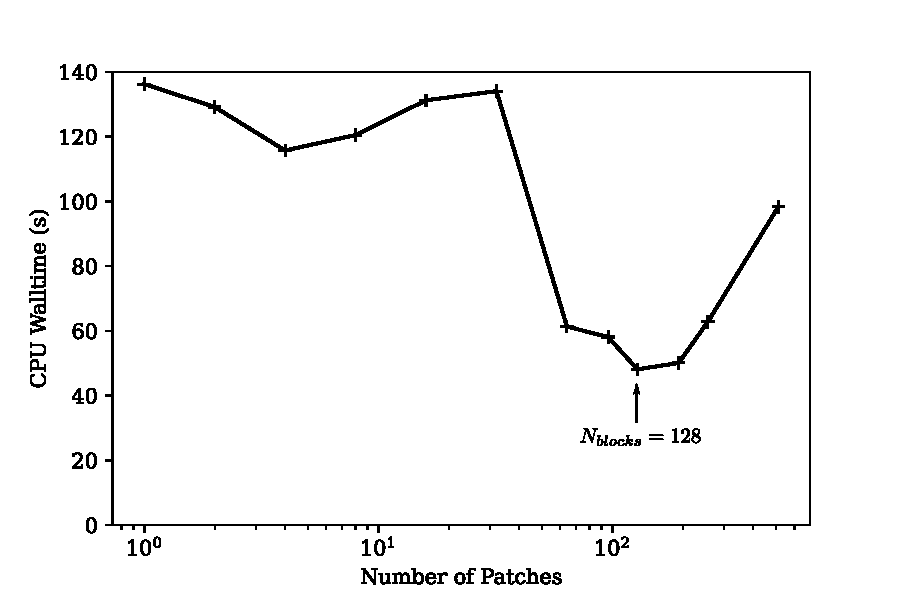
\includegraphics[width=0.8\textwidth]{cache_block_optimisation_annotated.pdf}
	\caption[Cache block optimisation]{Cache block optimisation. Total wall time of a test code for computing $\beta$s was measured while varying the number of cache blocks used. Having 128 blocks is optimal for the 18-core Intel Gold 6154 processor.}
	\label{fig:cache_block_optimisation}
\end{figure}

We find a significant improvement in performance moving from 32 to 48 blocks when the block size drops from 12MiB to 8MiB. This is precisely when three blocks are allowed to fit in L3 cache (24.7MiB) at the same time. Improved data locality dramatically reduces time spent on memory access as we expected. The optimal number of blocks was found to be 128; each segment contains about 400,000 elements and takes up 3MiB of memory, which is 1/6 and 1/8 of L2 and L3 cache size, respectively. We gain roughly three times speed-up compared to the original code without cache blocking.

Algorithm \ref{alg:beta_final_algorithm} summarises our final implementation of $\beta$ computation code, now with cache blocking and OpenMP construct indicators.

\begin{algorithm}[htbp]
	\caption{Computing $\beta$s: our final implementation}
	\label{alg:beta_final_algorithm}
	\begin{algorithmic}[1] % The number tells where the line numbering should start	
		\State Allocate $m(p,n)$ 
		\State Allocate $C(p_1,p_2,n)$ 
		\\\Comment{Both initialised within OpenMP construct over $n$}

		\For{each map $i$}
		\For{each mode $p$}
		\State \textbf{compute} $M(i,p,n)$ by SHT and store in $m(p,n)$
		\Comment{OpenMP within SHT}
		\EndFor
		\\
		\For{each block $b$}
		\For{each pair of modes $(p_1,p_2)$}
		\For{each pixel $n'$ in block}
		\Comment{OpenMP \textit{for} construct}
		\State $C(p_1,p_2,n') \pluseq m(p_1,n') \cdot m(p_2,n')$
		\EndFor
		\EndFor
		\EndFor
		\EndFor
		\Comment{$C(p_1,p_2,n)$ ready}
		\\
		\For{each map $i$}
		\For{each of mode $p$}
		\State \textbf{compute} $M(i,p,n)$ by SHT and store in $m(p,n)$
		\Comment{OpenMP within SHT}
		\EndFor
		\\
		\For{each block $b$}
		\For{each set of modes $(p_1,p_2,p_3)$}		
		\For{each pixel $n'$ in block}
		\Comment{OpenMP \textit{for} construct}
		\State $\beta^\text{cub}(i, p_1, p_2, p_3) \pluseq m(p_1,n') \cdot m(p_2,n') \cdot m(p_3,n')$
		\State $\beta^\text{lin}(i, p_1, p_2, p_3) \pluseq C(p_1, p_2, n') \cdot m( p_3, n')$
		\EndFor
		\EndFor
		\EndFor
		\EndFor
	\end{algorithmic}
\end{algorithm}

\section{Validation} \label{section:validation}

CMB bispectrum estimation is not only computationally challenging but also prone to numerical instabilities unless implemented carefully. We invested a considerable amount of time after the development of CMB-BEst in validating various aspects of the code. We highlight some of our validation efforts in this section, checking consistency within the program itself (section \ref{section:internal_consistency}) and against existing code such as Modal \cite{Fergusson2012} (section \ref{section:consistency_with_Planck}).

\subsection{Internal consistency checks} \label{section:internal_consistency}

CMB-BEst is a general code where one can freely choose a set of basis functions. Three of our main options are the `KSW' basis (\ref{eqn:KSW_basis}), `Legendre' basis (\ref{eqn:Legendre_basis_no_inv_k}, augmented with $q(k)=k^{n_\text{s}-2}$) as discussed previously in Section \ref{section:basis_functions}, and Fourier basis (\ref{eqn:Fourier_basis}). Both KSW and Legendre basis sets can cover the standard templates: local, equilateral, and orthogonal (see e.g., \cite{PlanckCollaboration2013} for definitions). The KSW basis provides an exact form for the three templates by choosing appropriate powers of $k$ as its basis elements. On the other hand, the templates are expanded in terms of separable Legendre polynomials up to some fixed degree $p_\text{max}$ for the Legendre basis. As long as $p_\text{max}$ is sufficiently large, most smooth bispectrum shapes can be represented accurately. 

Our first consistency check is shown in Figure \ref{fig:map_by_map_Legendre_KSW}, where we compare the $f_\text{NL}$ estimates from the Planck 2018 CMB map and 140 full focal plane (FFP10) realistic Gaussian simulations \cite{PlanckCollaboration2015simulations}. We use CMB maps obtained through the SMICA component separation method \cite{Cardoso2008component, PlanckCollaboration2013ComponentSeparation}. On the left hand side are scatter plots of $f_\text{NL}$ values obtained using each of the two basis sets. In an ideal case where the two estimates are identical for every test map, all the points would lie on a straight line given by $y=x$. Drawn in dashed red line is the best linear fit to the data. Its slope, intercept, and the $R$-squared value are annotated below. On the right is a more detailed plot of the computed $f_\text{NL}$ for each map.

\begin{figure}[htbp!] 
	\centering 
	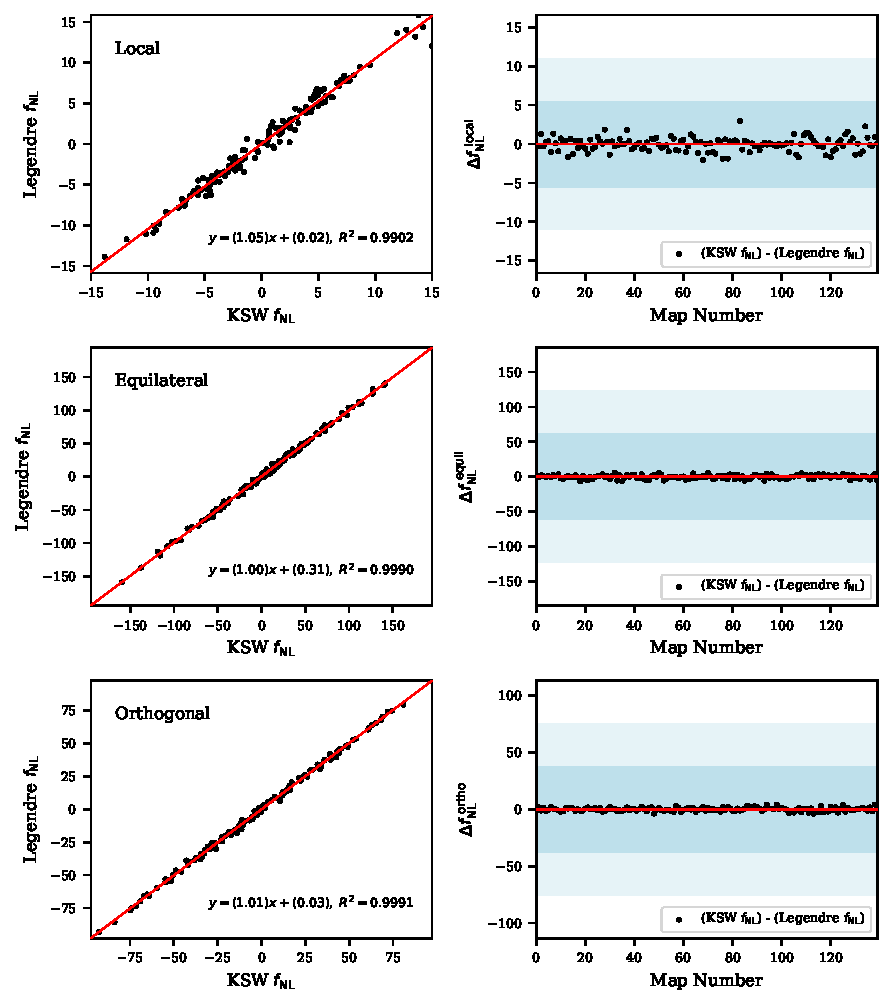
\includegraphics[width=\textwidth]{map_by_map_Legendre_KSW.pdf}
	\caption{Map-by-map comparison of $f_\text{NL}$ estimates for standard templates, evaluated using each of the KSW and Legendre basis sets. Planck 2018 CMB map and 140 FFP10 simulations have been used, each representing a single point on the scatter plot shown left. Details of the linear best-fit to data (red dashed) are annotated below. On the right hand side is shown a plot of $f_\text{NL}$ values for each map. In the ideal case where the two basis sets yield identical results, we should see all the points on $y=x$ for the left plot, and exactly overlapping graphs for the right. For more information on  each of the three theoretical templates used, see e.g., \cite{PlanckCollaboration2013}.}
	\label{fig:map_by_map_Legendre_KSW}
\end{figure}

We see that results from the two different sets of basis are in good agreement. The $R$-squared value of the linear fit is greater than $0.99$ for Local, and $0.999$ for Equilateral and Orthogonal shapes. The intercept and sample mean are also near zero. We do not find any systematic discrepancies across the shapes from individual map estimates either.

The fact that results from the KSW and Legendre basis are consistent validates multiple aspects of our pipeline. First of all, we can deduce that the Legendre basis expansion (\ref{eqn:basis_expansion}) accurately represents the bispectrum shapes of interest, especially since the KSW basis is designed to be exact for the three standard shapes. Having $p_\text{max}=30$ modes is more than sufficient. Figure \ref{fig:map_by_map_Legendre_30_29} explicitly compares results obtained from Legendre bases with $p_\text{max}=29$ and $30$, while keeping everything else the same. The two results show absolute agreement, the largest of errors less than $O(10^{-5})$. This further confirms that our expansion using Legendre polynomials has completely converged.

\begin{figure}[htbp!] 
	\centering    
	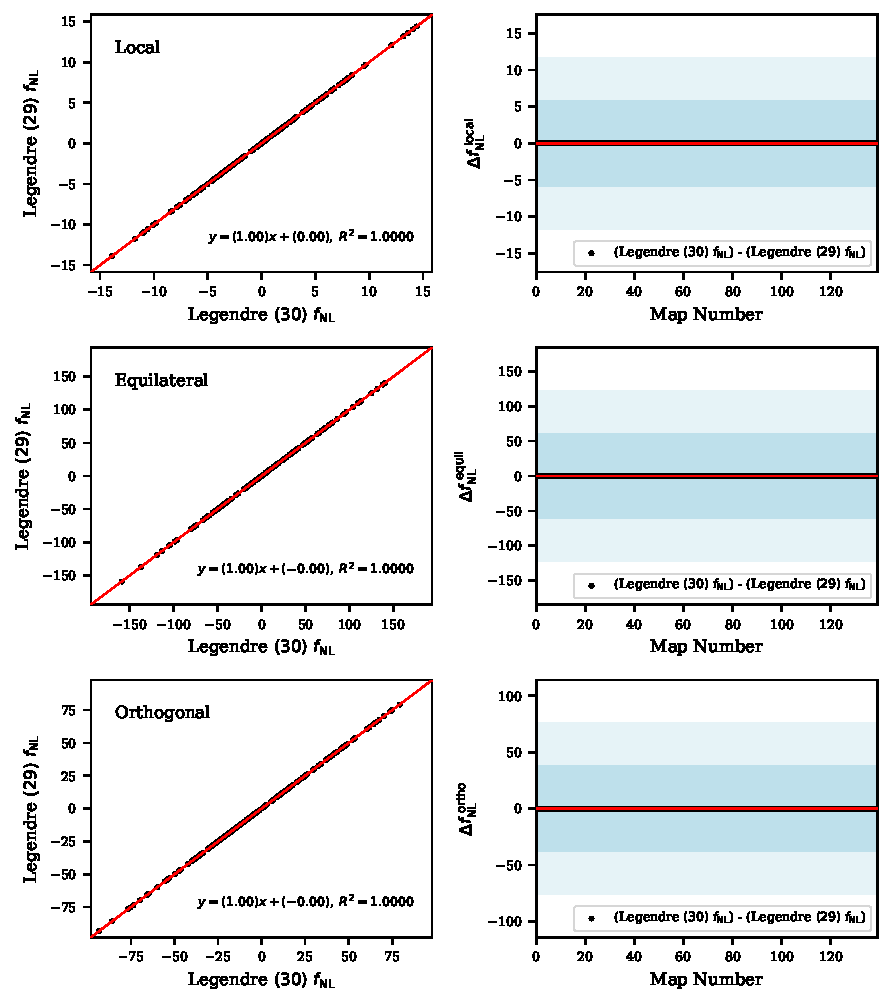
\includegraphics[width=\textwidth]{map_by_map_Legendre_30_29.pdf}
	\caption{Map-by-map comparison of $f_\text{NL}$ estimates for standard templates using the Legendre basis with different number of modes: $p_\text{max}=29$ and $30$. The two results agree with error less than $O(10^{-5})$, as can be seen from the scatter plots (left) and map-by-map plots (right). This confirms that our expansion using Legendre polynomials has completely converged for these bispectrum shapes.}
	\label{fig:map_by_map_Legendre_30_29}
\end{figure}

Secondly, we validated the accuracy of the linear term and lensing-ISW bias calculations through the sample mean of $f_\text{NL}$ estimates from lensed simulations. When we exclude either of the two, we find the sample mean to be far from zero. The error is especially large for the local template. The linear term accounts for the anisotropy introduced by masking parts of the observed sky. The squeezed limit contribution to bispectrum comes from couplings between a pair of small-scale modes and a large-scale one, making it more susceptible to bias from partial coverage. The presence of sky masks therefore offsets the $f_\text{NL}$ estimates from the local shape which has a large squeezed limit. Lensing-ISW bias is also the largest in squeezed configurations and affects Local $f_\text{NL}$. The fact that our lensed Gaussian simulations have $f_\text{NL}$s fluctuating around $0$ validates our bias subtractions.

Lastly, we check that CMB-BEst accurately preserves optimality of the CMB bispectrum estimator. In the weak non-Gaussian limit, the estimator (\ref{eqn:bispectrum_estimator_standard}) saturates the Cramer-Rao bound. Its expected variance is the lowest amongst all possible unbiased bispectrum estimators of $f_\text{NL}$. Heuristically speaking, the estimator extracts as much information about non-Gaussianity as possible from the CMB bispectrum. As we discussed in Chapter \ref{chapter:CMB_state-4_forecast}, this bound only depends on the Fisher information determined from normalisation; $Var[\hat{f}_\text{NL}]=F^{-1}=6/N$. We refer to this value as the \textit{theoretical} variance (the best possible from theory). Meanwhile, individual $f_\text{NL}$ estimates from simulated maps and independent and normally distributed. Sample variance obtained from $N_\text{sims}$ simulations should therefore approach the theoretical variance as $N_\text{sims}\rightarrow\infty$. Table \ref{table:trio_sample_and_theory_variances} summarises calculated values of the two types of variances discussed.

\begin{table}[h]
	\caption{Comparison of the sample and theoretical variances obtained from $f_\text{NL}$ estimates of standard shapes, computed using each of the KSW and Legendre basis sets. Sample variances are within $1\sigma$ of theoretical values assuming that the 140 individual $f_\text{NL}$'s from simulated maps are normally distributed. This is statistically consistent with optimality of our bispectrum estimator.}
	\centering
	\label{table:trio_sample_and_theory_variances}
	\renewcommand{\arraystretch}{1.5} 
	\begin{tabular}{llccc}
		\toprule
		Template & Basis & Sample Variance &  Theoretical Variance &  (Sample)/(Theory) \\
		\midrule
		\multirow{2}{*}{Local} & KSW &  5.5 &       5.3 &               1.04 \\
		& Legendre &             5.9 &                  5.7 &               1.04 \\
		\multirow{2}{*}{Equilateral} & KSW &            61.2 &                 67.7 &               0.90 \\
		& Legendre &            61.7 &                 67.7 &               0.91 \\
		\multirow{2}{*}{Orthogonal} & KSW &            37.7 &                 33.7 &               1.12 \\
		& Legendre &            38.0 &                 33.9 &               1.12 \\
		\bottomrule
	\end{tabular}
\end{table}

Note that the numbers do not match up exactly between sample and theoretical variances, and the results for equilateral template appear to be more optimal than the theory allows. This is because the sample variance $\hat{S}^2 = (\sum_i (f^{(i)}_\text{NL})^2 )/N_\text{sims}$ follows a chi-squared distribution with $N_\text{sims}-1$ degrees of freedom under our assumptions. The standard deviation corresponding to the (normalised) distribution equals $\sqrt{2/(N_\text{sims}-1)}$, which is $\approx 0.12$ for $N_\text{sims}=140$. It is therefore not surprising to see our sample variances differ by up to $12\%$ from the theoretical ones. 

We performed further checks to ensure that this discrepancy is due to statistical fluctuations rather than systematic errors. The ratio between sample and theoretical variances remained nearly constant across the KSW and Legendre basis from CMB-BEst, as well as Planck's Modal pipeline on the same set of simulated maps. Meanwhile, sample variances evaluated from independent sets of simulations do fluctuate around the theoretical value. A closer check has been done for each of the mode sets $(p_1,p_2,p_3)$ in the Legendre basis. The decomposition coefficient $\alpha$ is set to be 1 at $(p_1,p_2,p_3)$ and its permutations, and then vanishing everywhere else. Substituting into \eqref{eqn:fNL_from_betas} and \eqref{eqn:normlisation_from_gamma}, we get
\begin{align}
	f_\text{NL}^{(i)} &= \frac{1}{N} \left[ \left( \beta^{cub,(i)}_{p_1 p_2 p_3} - 3 \beta^{lin,(i)}_{p_1 p_2 p_3} \right) + \text{5 cyc.} \right], \\
	N &= 6\left( \Gamma_{p_1 p_2 p_3, p_1 p_2 p_3} + \Gamma_{p_1 p_2 p_3, p_1 p_3 p_2} + \cdots + \Gamma_{p_1 p_2 p_3, p_3 p_2 p_1} \right).
\end{align}
Here we assumed that $p_1,p_2,p_3$ are distinct for convenience. Corresponding sample and theoretical variances have been compared for each of the modes. Overall, they are found to be statistically consistent as before.

% Optional: could include a historgram plot for (sample var)/(theory var) calculated for each of the modes (p1,p2,p3) in Legendre basis. p_max = 30 would make the plot look sufficiently smooth...

While Figure \ref{fig:map_by_map_Legendre_KSW} shows excellent agreement between results from the KSW and Legendre basis sets overall, there are small but noticeable scatters in the plot for the local shape. The slope of linear best fit is also slightly above 1, meaning that $f_\text{NL}$ estimates from the Legendre routine tend to vary 5\% more than the KSW ones. Larger variance means that less information extracted. Our first hypothesis was that Legendre polynomials are losing a small fraction of information due to their fixed $k$ range in their definition ($\ref{eqn:Legendre_basis_no_inv_k}$). We test this by increasing the range by changing $k_\text{max}/k_\text{min} = 1000$ to $2000$. The results are shown in Figure \ref{fig:map_by_map_Legendre_KSW_k_ratio_2000}.

\begin{figure}[htbp!] 
	\centering    
	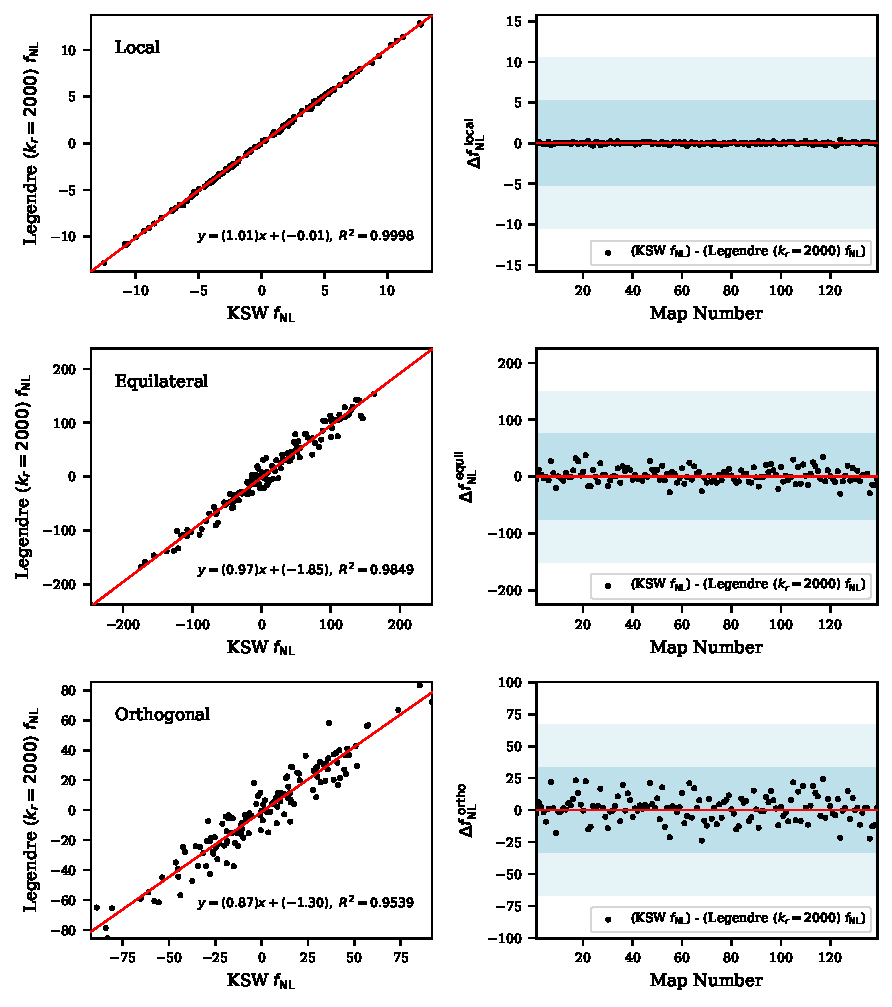
\includegraphics[width=\textwidth]{map_by_map_Legendre_KSW_k_ratio_2000.pdf}
	\caption{Map-by-map comparison of $f_\text{NL}$ estimates for standard templates from the KSW and Legendre basis sets, similar to Figure \ref{fig:map_by_map_Legendre_KSW}. Here, the Legendre basis has a wider $k$ domain: $k_\text{max}/k_\text{min} = 2000$ instead of the usual $1000$. The number of modes ($p_\text{max}$) has been reduced to $10$ instead of $30$ due to limited computational resources. We see that additional information from large scales (low $k$) fixes the small scatter present in $f_\text{NL}^{local}$ of the previous plot.}
	\label{fig:map_by_map_Legendre_KSW_k_ratio_2000}
\end{figure}

Our main focus of this figure is on the local template results. Estimates from the KSW and Legendre basis sets match almost perfectly now. When altering the ratio $k_\text{max}/k_\text{min}$, we fixed the $k_\text{max}$ and lowered $k_\text{min}$. Including more small-$k$, or large scale modes provides extra information in the bispectrum. Local shape is especially affected by this, since squeezed configurations including one of these extra large scale modes have a more significant contribution to the total estimate. Also note that $k_\text{max} / k_\text{min} = 2000$ is comfortably larger than the equivalent ratio in harmonic space $l_\text{max} / l_\text{min} = 2500 / 2$.

Despite the improvements in the squeezed limit and local template, we may not simply set $k_\text{max} / k_\text{min} = 2000$ as default because it hurts convergence in other shapes of interest. As can be seen from the Equilateral and Orthogonal plots in Figure \ref{fig:map_by_map_Legendre_KSW_k_ratio_2000}, newer estimates of $f_\text{NL}$ are less accurate for shapes other than Local. The fact that $p_\text{max}=10$ here rather than $30$ is one of the main causes of the drop in precision, but having smaller $k$ values within Legendre polynomials' domain also has a negative impact. Shapes with inverse $k$ scaling vary more dramatically when $k$ is small and tend to be harder to expand in terms of Legendre polynomials.

For the final check of internal consistency, we inspect how each point in the line of sight integral ($r$) contributes to $f_\text{NL}$ estimates. CMB-BEst's formalism makes it straightforward to plot the $r$ integrand since the integral is done at the very end. Figure \ref{fig:trio_r_dependence} shows plots of $f_\text{NL}$ contributions from different sources and for the three standard bispectrum templates. Shaded in light blue are the $1\sigma$ regions obtained from 140 simulations for each point in $r$.

\begin{figure}[htbp!] 
	\centering    
	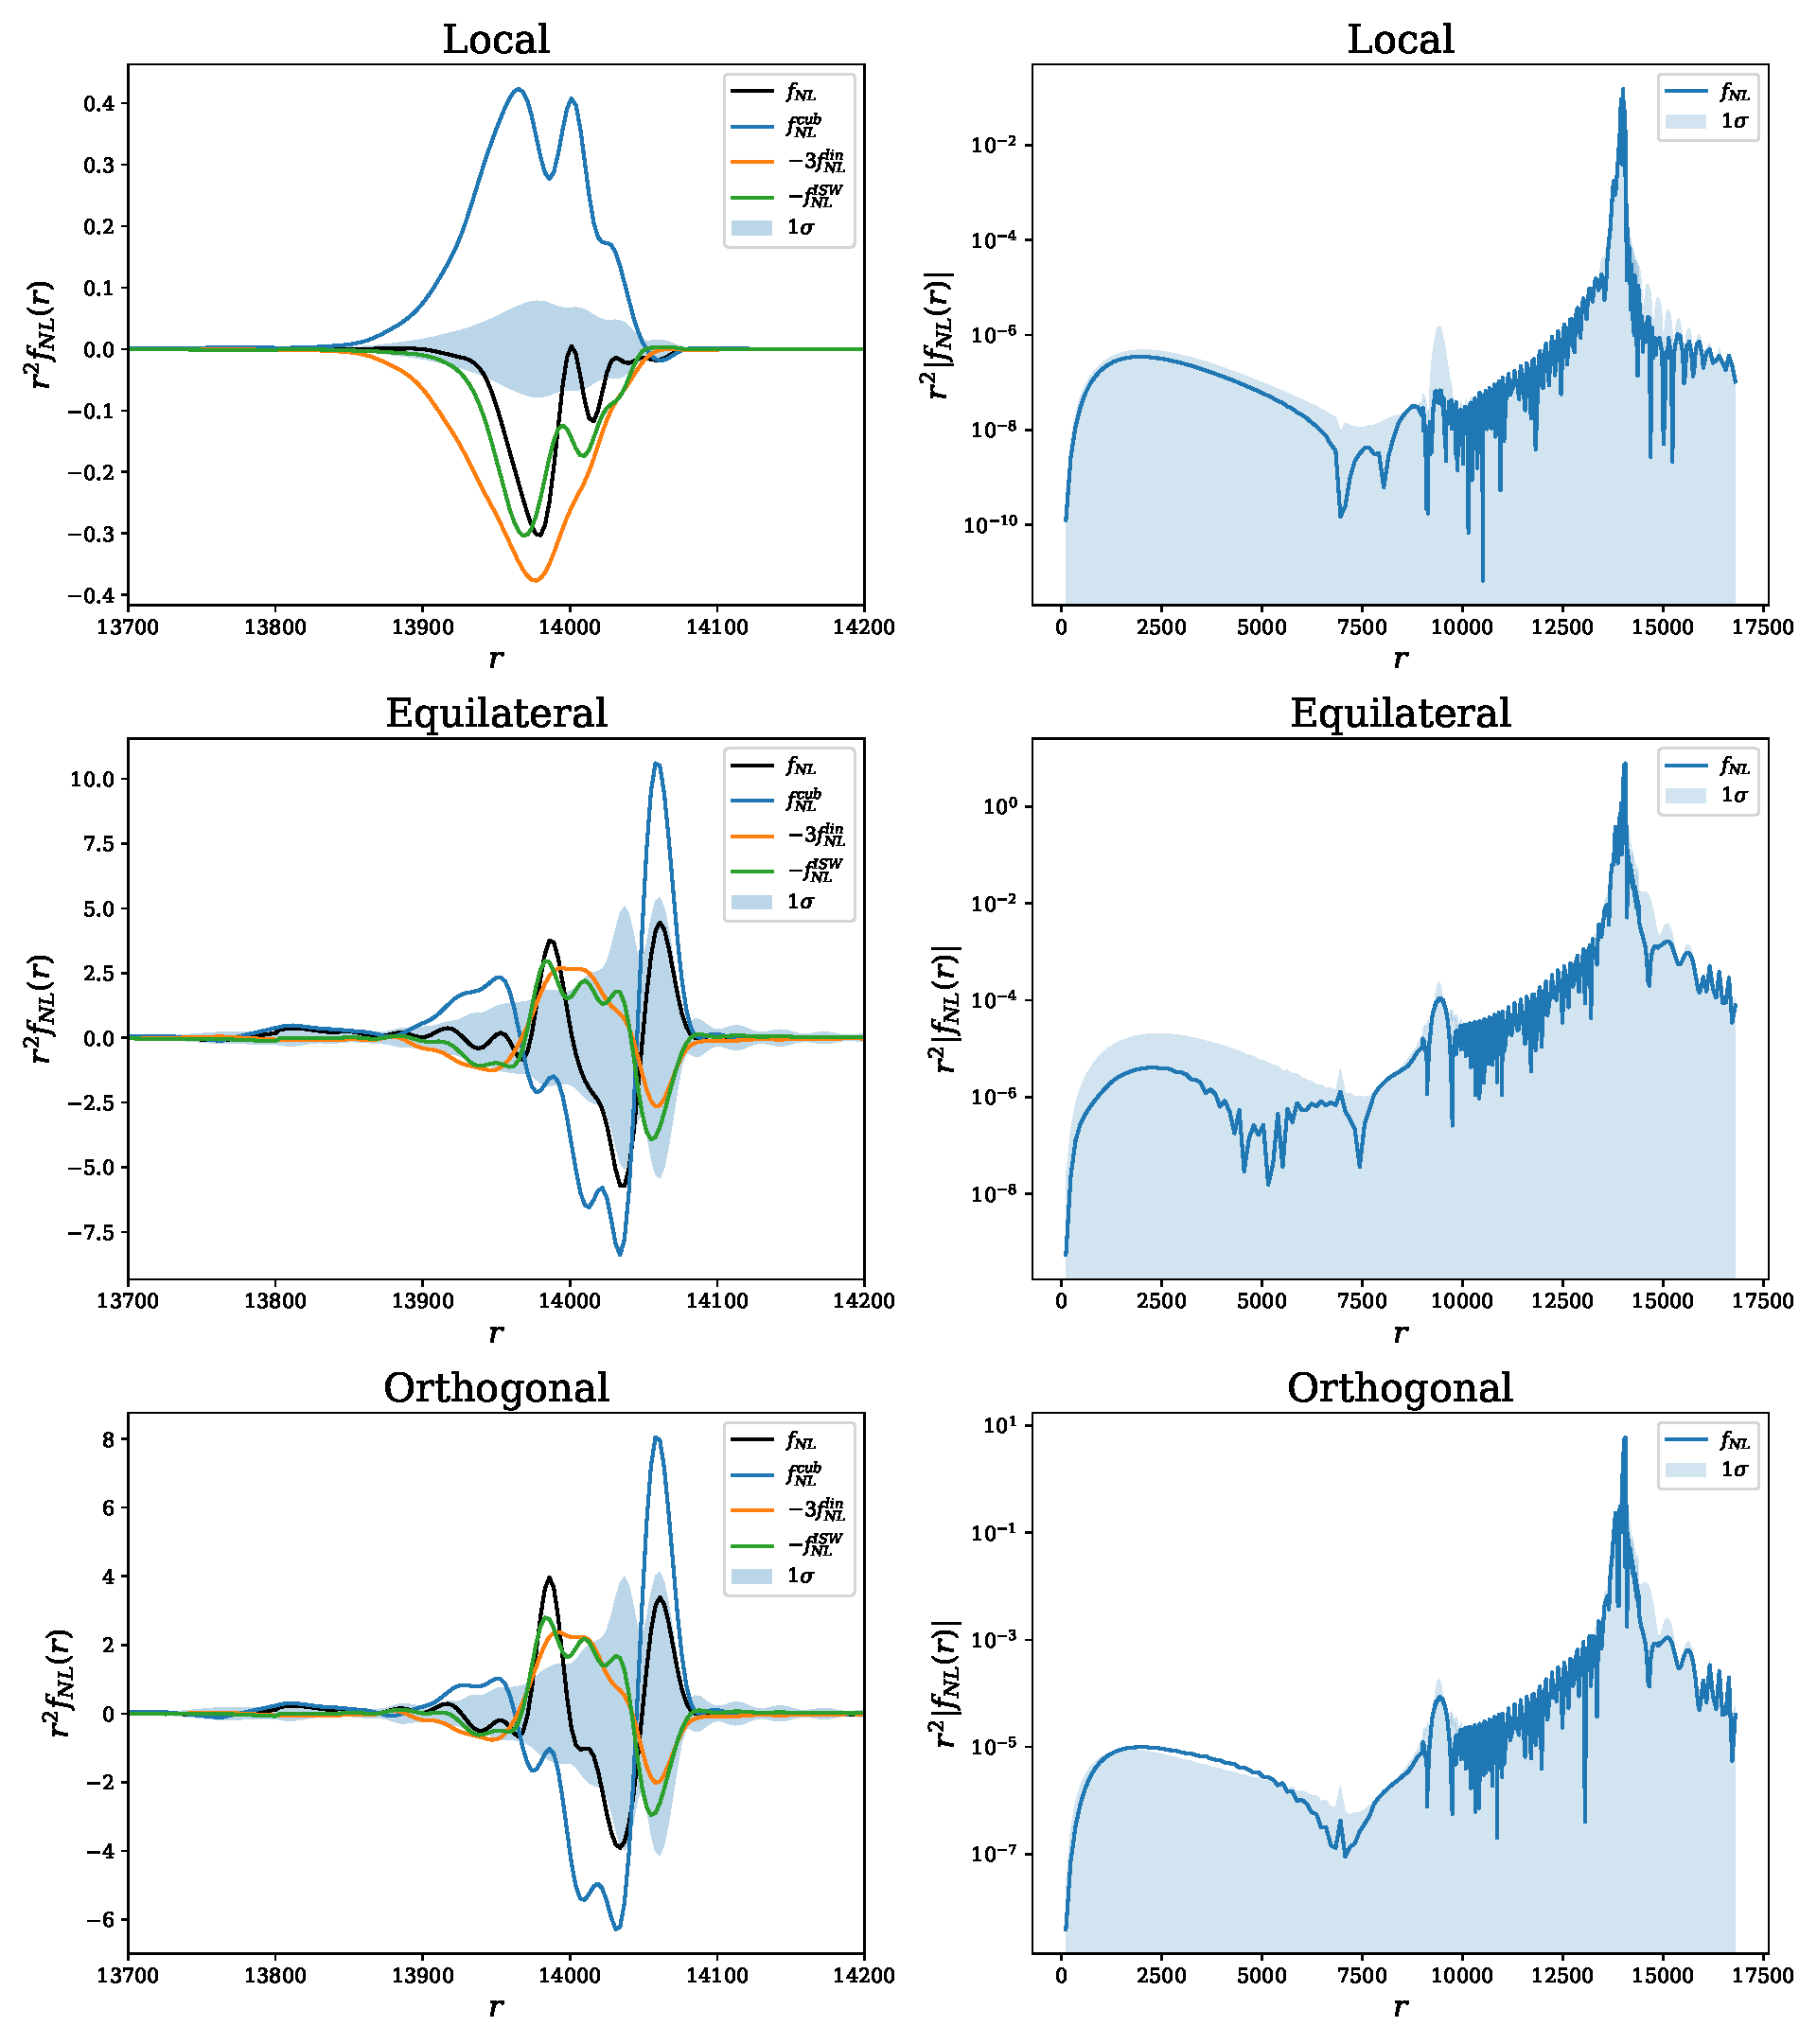
\includegraphics[width=\textwidth]{trio_r_dependence.pdf}
	\caption{Contributions to the total $f_\text{NL}$ from each point in the line-of-sight integral over $r$ for standard templates. On the left hand side, we plot contributions from the cubic, linear, and lensing-ISW bias, as well as the total $f_\text{NL}$. Shown in blue is the $1\sigma$ interval obtained from corresponding terms in 140 FFP10 Gaussian simulations. We focus on the $r$ interval around recombination where most of the signal comes from. Plots on the right hand side show $f_\text{NL}$ contributions over the whole $r$ range in log scale. ISW effect, reionisation, and recombination are responsible for the three most noticeable peaks in all three plots.}
	\label{fig:trio_r_dependence}
\end{figure}

As illustrated in plots on the right hand side of Figure \ref{fig:trio_r_dependence}, the vast majority of signal comes from recombination around $r = 14,000$Mpc. In fact, its contribution is dominant enough so that neglecting signal from everywhere else would still be a good approximation. CMB-BEst uses an adaptive $r$ grid which is denser around recombination, following the works of \cite{Smith2011}. Other small but notable contributions to the total estimate comes from reionisation ($r \sim 10,000$Mpc) and the ISW effect ($r < 5,000$Mpc).

Zooming in on an interval around recombination, significant contributions from the cubic term to $f_\text{NL}$ of Local template is rather prominent (upper left of Figure \ref{fig:trio_r_dependence}). The signal is sufficiently larger than the expected random fluctuations evaluated from Gaussian simulations, which could be hinting at non-zero primordial non-Gaussianity. However, contributions from the linear term (shown orange) completely counterbalances it, bringing the total down to values consistent with zero. This again validates accuracy of our methodology; bias to $f_\text{NL}$ generated from anisotropic sky masks are precisely subtracted off using the linear terms.

We do not find any statistically significant signal across the whole $r$ range otherwise, especially when taking look-elsewhere effect into account. It is not meaningful to find a couple of 3-4$\sigma$ values when the other 500 points are simply disregarded. If we detect primordial non-Gaussianity in the future, however, then these plots of $f_\text{NL}$ contributions for each $r$ will provide valuable insights on where the signal comes from.

% Write about convergecne? 
%- Convergence epsilon definition
%- Standard templates convergence epsilons
%- Legendre - constant feature models part. Correlation matrix


\subsection{Consistency with Planck} \label{section:consistency_with_Planck}

In the previous section, we demonstrated how the integrity of CMB-BEst was validated. The next set of validations involves comparing it against other existing codes for CMB bispectrum estimation.

We test primordial non-Gaussianity constraints on Local, Equilateral and Orthogonal templates against the Planck 2018 analysis \cite{PlanckCollaboration2018}. Two sets of basis functions, KSW and Legendre, have been used to compute $f_\text{NL}$ from the foreground-cleaned CMB map included in the final data release. We choose SMICA as the main component separation method since it was shown to be the most reliable and robust for Planck bispectrum analysis \cite{PlanckCollaboration2013ComponentSeparation, PlanckCollaboration2013,PlanckCollaboration2015,PlanckCollaboration2018}. Table \ref{table:trio_fNL_comparison_with_planck} summarises the constraints obtained, together with the quoted results from the Planck team's own KSW estimator and Modal 2 pipeline.

\begin{table}[h]
	\caption{Constraints on $f_\text{NL}$ for the standard shapes from the KSW and Legendre basis of CMB-BEst, in comparison with the Planck 2018 analysis \cite{PlanckCollaboration2018}. Only temperature data from the SMICA foreground-cleaned map and FFP10 simulations were used for the analysis. Values shown are after the lensing bias subtraction, with uncertainties at 68\% CL.}
	\centering
	\label{table:trio_fNL_comparison_with_planck}
	\renewcommand{\arraystretch}{1.5} 
	\begin{tabular}{lcccc}
		\toprule
		& \multicolumn{2}{c}{CMB-BEst} & \multicolumn{2}{c}{Planck 2018} \\ \cmidrule(lr){2-3} \cmidrule(lr){4-5}
		Shape & KSW &  Legendre &  KSW &  Modal \\
		\midrule
		
		Local & $-2.2 \;\pm\; 5.5$ & $-2.0 \;\pm\; 5.9$ & $-0.5 \;\pm\; 5.6$ & $-0.6 \;\pm\; 6.4$ \\
		Equilateral & $17 \;\pm\; 61$ & $15 \;\pm\; 62$ & $7 \;\pm\; 66$ & $34 \;\pm\; 67$ \\
		Orthogonal & $-7 \;\pm\; 38$ & $-9 \;\pm\; 38$ & $-15 \;\pm\; 36$ & $-26 \;\pm\; 43$ \\
		\bottomrule
	\end{tabular}
\end{table}

Note that while the constraints from CMB-BEst are largely consistent with Planck 2018 results, there are discrepancies of up to $0.3\sigma$. However, there are variations around this level within the estimates from different pipelines of Planck as well. Equilateral constraints from Planck's own KSW and Modal estimators shown here, for example, differ by $\approx 0.4\sigma$. A similar amount of fluctuation can be found in the full result shown in \cite{PlanckCollaboration2018}. In an ideal world, they should match exactly across different approaches as long as the same dataset is used. However, statistical significance of the individual $f_\text{NL}$'s is not largely affected by such variations.

We invested a significant proportion of our time investigating this error. Here we discuss three potential areas which might account for the discrepancies. First of all, human error during the implementation and estimation process should not be neglected. Bispectrum analysis is complex and computationally expensive. Implementing it often involves writing a long and heavily optimised code. During the development and testing stages, we found and fixed many mistakes in our $10,000+$ lines of \textsc{C} code. Various unit tests were performed in the process to test individual sections of the code: basis expansion, projection to the $l$ space, SHTs, parallelisation, and more. Internal consistency checks were then used to verify integrity of the combined pipeline. The Planck team also went to great lengths to validate and cross-check different methods \cite{PlanckCollaboration2013}. It therefore seems unlikely that trivial mistakes are causing the gap in results.

The next source of error we studied is the parameter set. The cosmological parameters we used for constraints in Table \ref{table:trio_fNL_comparison_with_planck} are identical to those of the Planck Modal pipeline. Small changes in cosmological parameters are also shown to have little effect on $f_\text{NL}$ \cite{PlanckCollaboration2015,PlanckCollaboration2018}. One major difference, however, is the number of Gaussian simulations used. We included 140 simulated maps while Modal has about 300. This number is mainly restricted by computational resources required for the large Legendre basis in CMB-BEst. While we found 140 to be sufficient for most cases, sample variance may cause some fluctuation in the linear term and error bar. A rough estimate for sampling error is $\sim \sqrt{2/N_\text{sims}} \approx 0.12$, as calculated in the previous section. Other than $N_\text{sims}$, more internal parameters such as the grid density of discretised arrays have also been checked to yield consistent results when varied. 

We are left with systematic errors as potential causes for discrepancies. The most significant bias to $f_\text{NL}$ constraints is the lensing-ISW bias discussed in Section \ref{section:other_sources_of_non_gaussianity}. Table \ref{table:trio_lensing_bias_comparison_with_planck} shows biases from the lensing bispectrum \cite{Lewis2011lensing} for both CMB-BEst and Planck 2018 analysis. The numbers vary but are consistent overall. Map-by-map comparison of constraints from the Legendre basis and Modal are shown in Figure \ref{fig:map_by_map_Legendre_Modal}. 

\begin{table}[h]
	\caption{Bias to $f_\text{NL}$ of standard shapes originating from the lensing bispectrum. We compare CMB-BEst's two different basis sets and the Planck 2018 analysis \cite{PlanckCollaboration2018}, using SMICA map and FFP10 simulations. }
	\centering
	\label{table:trio_lensing_bias_comparison_with_planck}
	\renewcommand{\arraystretch}{1.5} 
	\begin{tabular}{lcccc}
		\toprule
		& \multicolumn{2}{c}{CMB-BEst} & \multicolumn{2}{c}{Planck 2018} \\ \cmidrule(lr){2-3} \cmidrule(lr){4-5}
		Shape & KSW &  Legendre &  KSW &  Modal \\
		\midrule
		
		Local & $7.5$ & $8.2$ & $7.3$ & $6.9$ \\
		Equilateral & $-0.7$ & $-0.6$ & $-0.7$ & $4.0$\\
		Orthogonal & $-22$ & $-22$ & $-23$ & $-25$ \\
		\bottomrule
	\end{tabular}
\end{table}

\begin{figure}[htbp!] 
	\centering    
	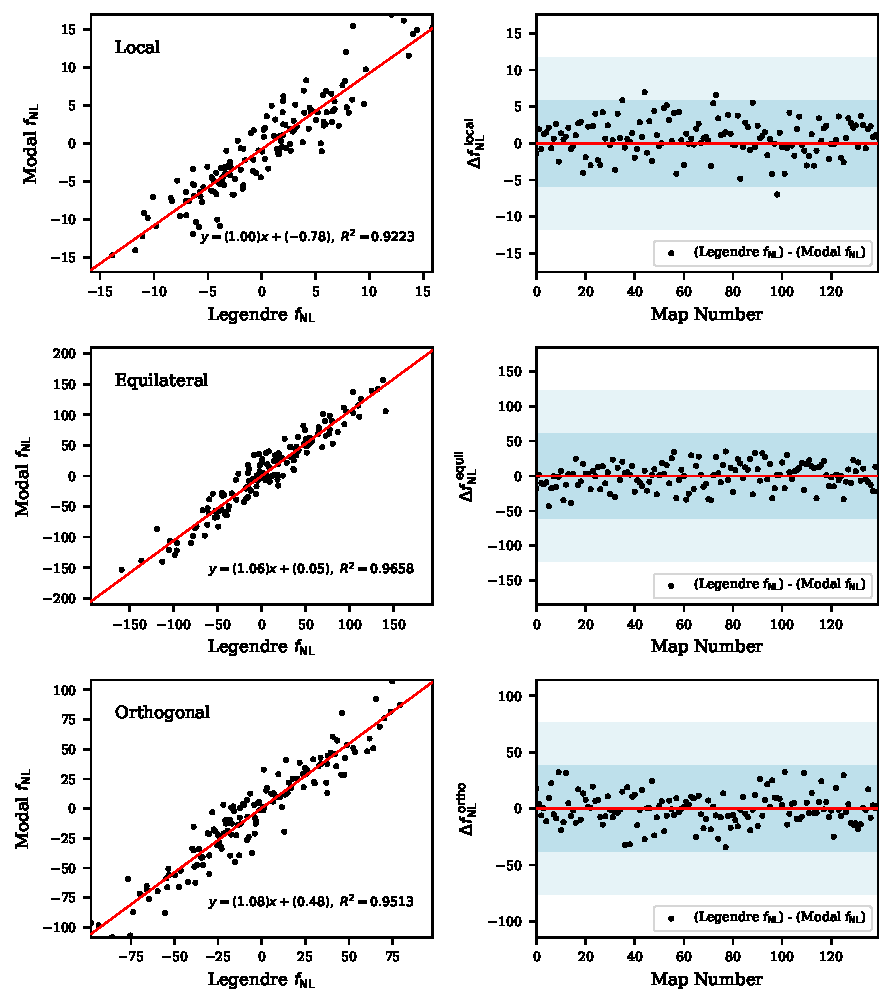
\includegraphics[width=\textwidth]{map_by_map_Legendre_Modal.pdf}
	\caption{Map-by-map comparison of $f_\text{NL}$ estimates obtained from CMB-BEst's Legendre basis set against the Modal estimator results for Planck 2018 analysis \cite{PlanckCollaboration2018}. The first 140 FFP10 simulations are used. On the left hand side are scatter plots where each simulation is represented by a point according to $f_\text{NL}$ estimates of standard templates. Their linear best fit lines are shown in dashed red. Results from the two routines are shown map-by-map on the right hand side. Overall, CMB-BEst and Modal are in good agreement without any significant systematic errors.}
	\label{fig:map_by_map_Legendre_Modal}
\end{figure}

Out of the three templates, local shape shows the largest scatter between constraints. Comparing $f_\text{NL}$'s of simulated maps from CMB-BEst and Modal, we find a correlation of 0.916. The intercept value of $0.78$ in the linear fit is mainly due to the sample mean present in Modal. Legendre's sample mean is $0.069$ for Local, while Modal's is $-0.698$. Otherwise, the difference between the two pipelines are distributed such that its sample standard deviation equals $2.5$, skewness is $-0.14$, and kurtosis is $0.19$. Having a low level of small skewness and kurtosis less than $1$ implies that the distribution is close to a univariate normal, consistent with random fluctuation. Similarly, we do not find any significant systematic error from the equilateral and orthogonal shapes either.

Having not found a clear source of error, we conclude that the small gaps between the $f_\text{NL}$ estimates in Table \ref{table:trio_fNL_comparison_with_planck} mainly come from differences in methodology and are consistent with random fluctuations.

We now move on to constraining models with oscillations. The simplest template for oscillatory models is the feature model studied in Chapter \ref{chapter:CMB_state-4_forecast}. We use a template shape function of the form $S^\text{feat}(k_1,k_2,k_3) = \sin(\omega (k_1 + k_2 + k_3) + \phi)$. Figure \ref{fig:sine_template_frequency_Legendre_Modal} shows $f_\text{NL}$ constraints obtained from the Legendre basis and compares them with Modal results from the Planck 2018 analysis. The `phase' $\phi$ is set to zero, while oscillation `frequency' $\omega$ was varied from $10$ Mpc to $350$ Mpc. We follow \cite{Fergusson2015a} and increase $\omega$ in steps of $10$ so that correlation between shapes with different $\omega$ is kept low.

\begin{figure}[htbp!] 
	\centering    
	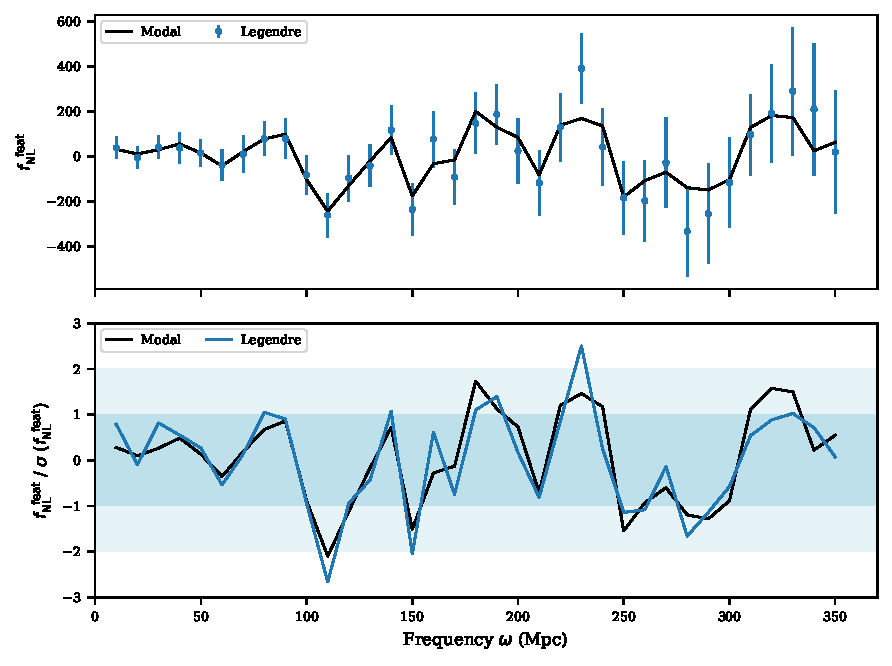
\includegraphics[width=\textwidth]{sine_template_frequency_Legendre_Modal.pdf}
	\caption{Estimated $f_\text{NL}$'s for feature models with shape $S(k_1,k_2,k_3) = \sin(\omega (k_1 + k_2 + k_3)$, obtained using the Legendre basis with (blue) and Planck's Modal (black). Left: direct comparison of $f_\text{NL}$ for different values of $\omega$. Error bars indicate the expected standard deviation in the estimator, calculated using 140 Gaussian simulations. Right: measured signal-to-noise $f_\text{NL}/\sigma$, again for a range of $\omega$ values. Shaded in blue are the $1\sigma$ and $2\sigma$ levels. We see that the two approaches yield coherent estimates overall.}
	\label{fig:sine_template_frequency_Legendre_Modal}
\end{figure}

The Legendre basis accurately expands the feature model template using Legendre polynomials via basis expansion outlined in (\ref{eqn:basis_expansion}). Estimates from the two methods, CMB-BEst's Legendre and Planck's Modal, are mostly compatible. The most notable difference is at $\omega=230$Mpc where $f_\text{NL}$ from Legendre is more than $1\sigma$ larger compared to Modal. Even though it is interesting that the new estimate now passes the $2\sigma$ threshold, having one such point out of 35 shown here has less statistical significance.

Both the Legendre and Modal approaches involve expanding the shape function with respect to a polynomial basis. Polynomials are versatile but have limited resolution for oscillatory signals; it cannot resolve shapes with a number of oscillations greater than the maximum degree of polynomials ($p_\text{max}$ here). For the Legendre basis with $k$ range $[2.09\times 10^{-4}, 2.09\times 10^{-1}]\text{Mpc}^{-1}$ and $p_\text{max}=30$, frequencies greater than $\pi p_\text{max} / (k_\text{max} - k_\text{min}) \approx 436$Mpc are unresolvable. In reality, numerics start to break before this value. We do not have a reference analytic value for true $f_\text{NL}$s, but evaluating correlations between shapes is effective for checking our numerics.

\begin{figure}[htbp!] 
	\centering    
	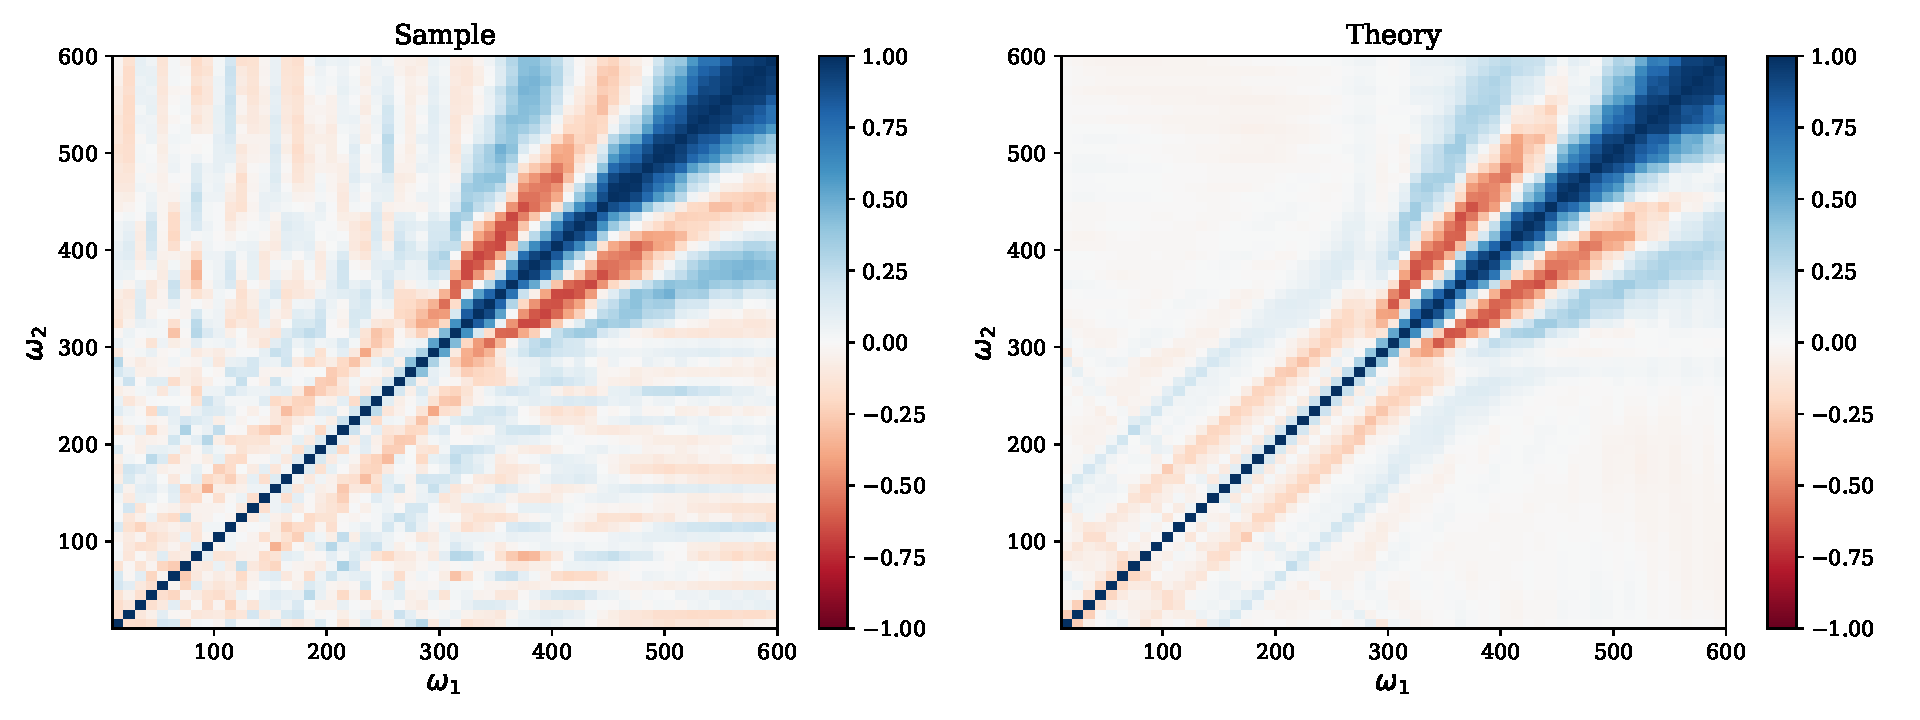
\includegraphics[width=\textwidth]{sine_template_correlations_new.pdf}
	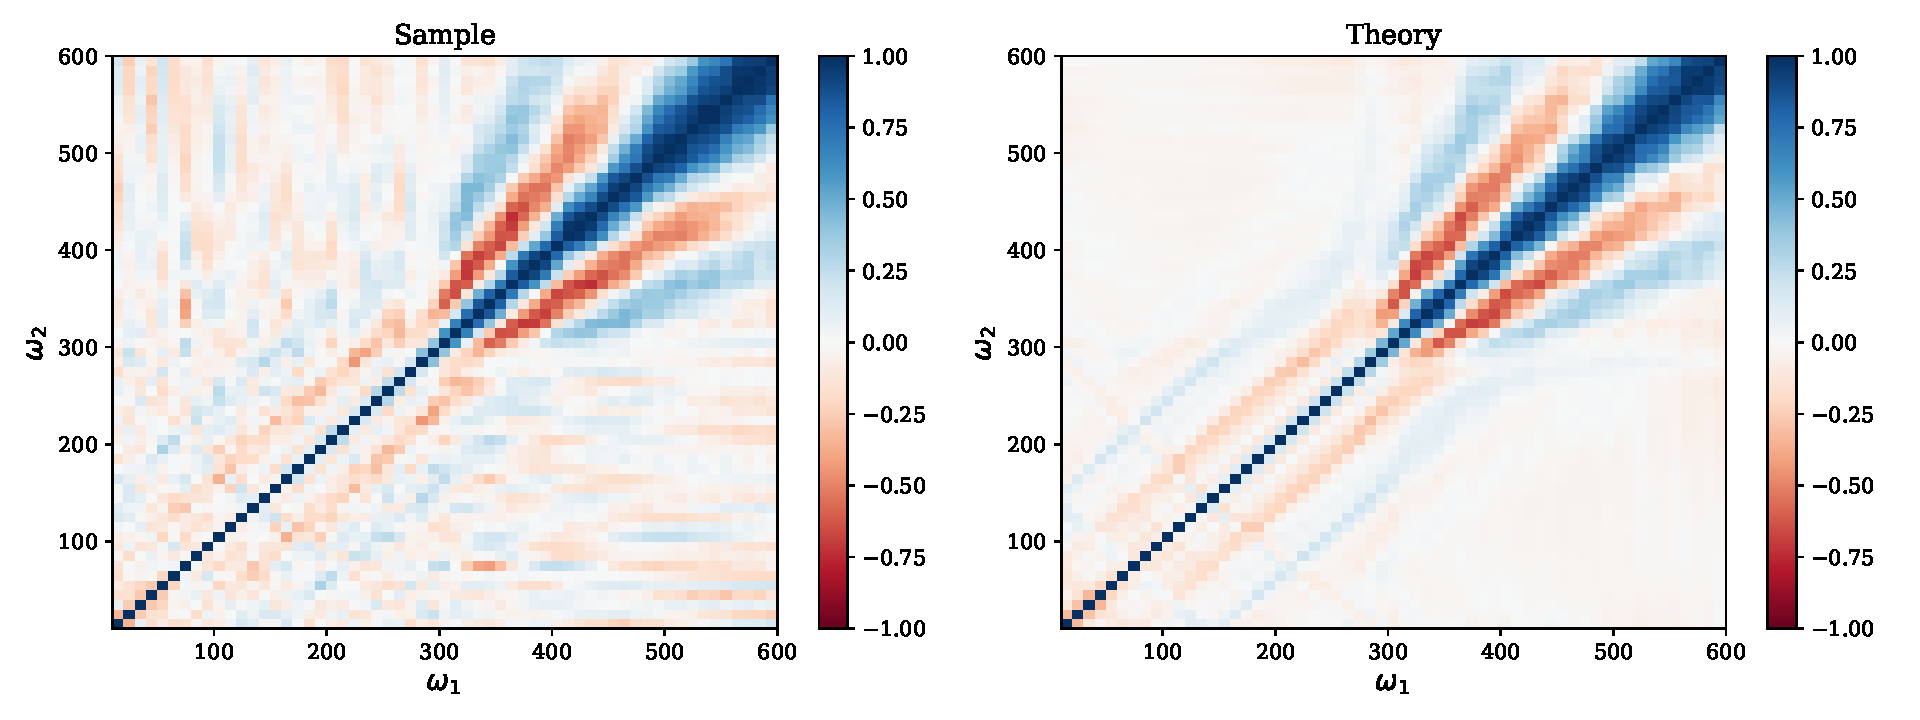
\includegraphics[width=\textwidth]{cosine_template_correlations_new.pdf}
	\caption{Correlations between feature model templates $S(k_1,k_2,k_3)=\sin(\omega (k_1 + k_2 + k_3) + \phi)$ with different $\omega$ values, for $\phi = 0$ (top two) and $\phi = \pi/2$ (bottom two). Results are from the Legendre basis. `Sample' correlations are obtained from $f_\text{NL}$ estimates from 140 Gaussian simulations, while `theory' correlations come from the inner product induced by $\Gamma_{p_1 p_2 p_3, p_1 p_2 p_3}$ matrix in (\ref{def:gamma}). Large non-diagonal correlations appear around $\omega \approx 300$, after which oscillations in the shape are no longer resolved by polynomials of degree up to $p_max$.}
	\label{fig:feature_template_correlations}
\end{figure}

Figure \ref{fig:feature_template_correlations} shows correlations between $f_\text{NL}$s from feature models with different frequency $\omega$s. The plots show correlation between $f_\text{NL}$ estimates from 140 FFP10 Gaussian simulations (`sample'), together with the one evaluated using our `late-time' inner product ('theoretical') given by
\begin{align}
	\left< b^{(i)}, b^{(j)} \right> &= \sum_{l_j} \frac{h^2_{l_1 l_2 l_3} b^{(i)}_{l_1 l_2 l_3} b^{(j)}_{l_1 l_2 l_3}}{C_{l_1} C_{l_2} C_{l_3}}  \\
	&= \sum_{p_j p'_j} \alpha^{(i)}_{p_1 p_2 p_3} \alpha^{(j)}_{p'_1 p'_2 p'_3} \sum_{l_j} \frac{h^2_{l_1 l_2 l_3} (b^{(i)}_{p_1 p_2 p_3})_{l_1 l_2 l_3} (b^{(j)}_{p'_1 p'_2 p'_3})_{l_1 l_2 l_3}}{C_{l_1} C_{l_2} C_{l_3}} \\
	&= \sum_{p_j p'_j} \alpha^{(i)}_{p_1 p_2 p_3} \alpha^{(j)}_{p'_1 p'_2 p'_3} \Gamma_{p_1 p_2 p_3, p'_1 p'_2 p'_3} \\
	&= \vv{\alpha^{(i)}} \; \Gamma \; \vv{\alpha^{(j)}}, \label{eqn:late_time_inner_product}
\end{align}
where $\Gamma$ is defined in (\ref{def:gamma}). In the limit $N_\text{sims} \rightarrow \infty$, the sample correlation can be shown to approach the theoretical value in the weakly non-Gaussian limit. We see from Figure \ref{fig:feature_template_correlations} that they indeed display the same qualitative behaviour for $N_\text{sims}=140$.

The templates with $\omega < 300$ are highly uncorrelated with each other, as can be seen from small non-diagonal elements. Noticeable correlations on lines $\omega_2 = \omega_1 \pm c$ for $c = 70, 140$ arise from resonance between oscillations and transfer functions at the Baryonic Acoustic Oscillation (BAO) scale, as we observed in Figure \ref{insight feature plot}. Faint lines can also be found near $\omega_2 = -\omega_1 + c, \;\; c = 70,140,210,\cdots$ for similar reasons.

When $\omega > 300$, however, large non-diagonal correlations appear. This is about when the oscillation frequency surpasses the resolution set by the highest degree of polynomials. Our basis expansion becomes inaccurate after this point. There are interesting linear structures present, with slopes roughly equal to $2, 1/2$ and subsequently $4, 1/4$. These lines come from aliasing caused by subsampling rapid oscillations; our basis picks up $\omega' = \omega/2$ signal instead. $\omega_2/2 = -\omega_1 + 70$ and other pairs of $(\omega_1, \omega_2)$ resonate to give large non-diagonal correlations.

We verify our claim that numerical inaccuracies at high $\omega$s are caused by the lack of resolution due to a limited number of polynomial modes. Figure \ref{fig:feature_template_correlations_compare_lmax} illustrates how having a smaller $k$ range allows us to constrain faster oscillations more accurately. Note that we also change $l_\text{max}$ correspondingly since smaller scales are neglected. The plot on the right hand side uses a Legendre basis with the $(k_\text{min}, k_\text{max})$ range rescaled by a factor of $3/4$. Fewer oscillations appear within the $k$ interval and are therefore easier to expand using fewer polynomials. As we expected, the scale at which non-diagonal correlations blow up is now shifted to a higher frequency, $\omega \approx (4/3) \cdot 300$. 

\begin{figure}[htbp!] 
	\centering    
	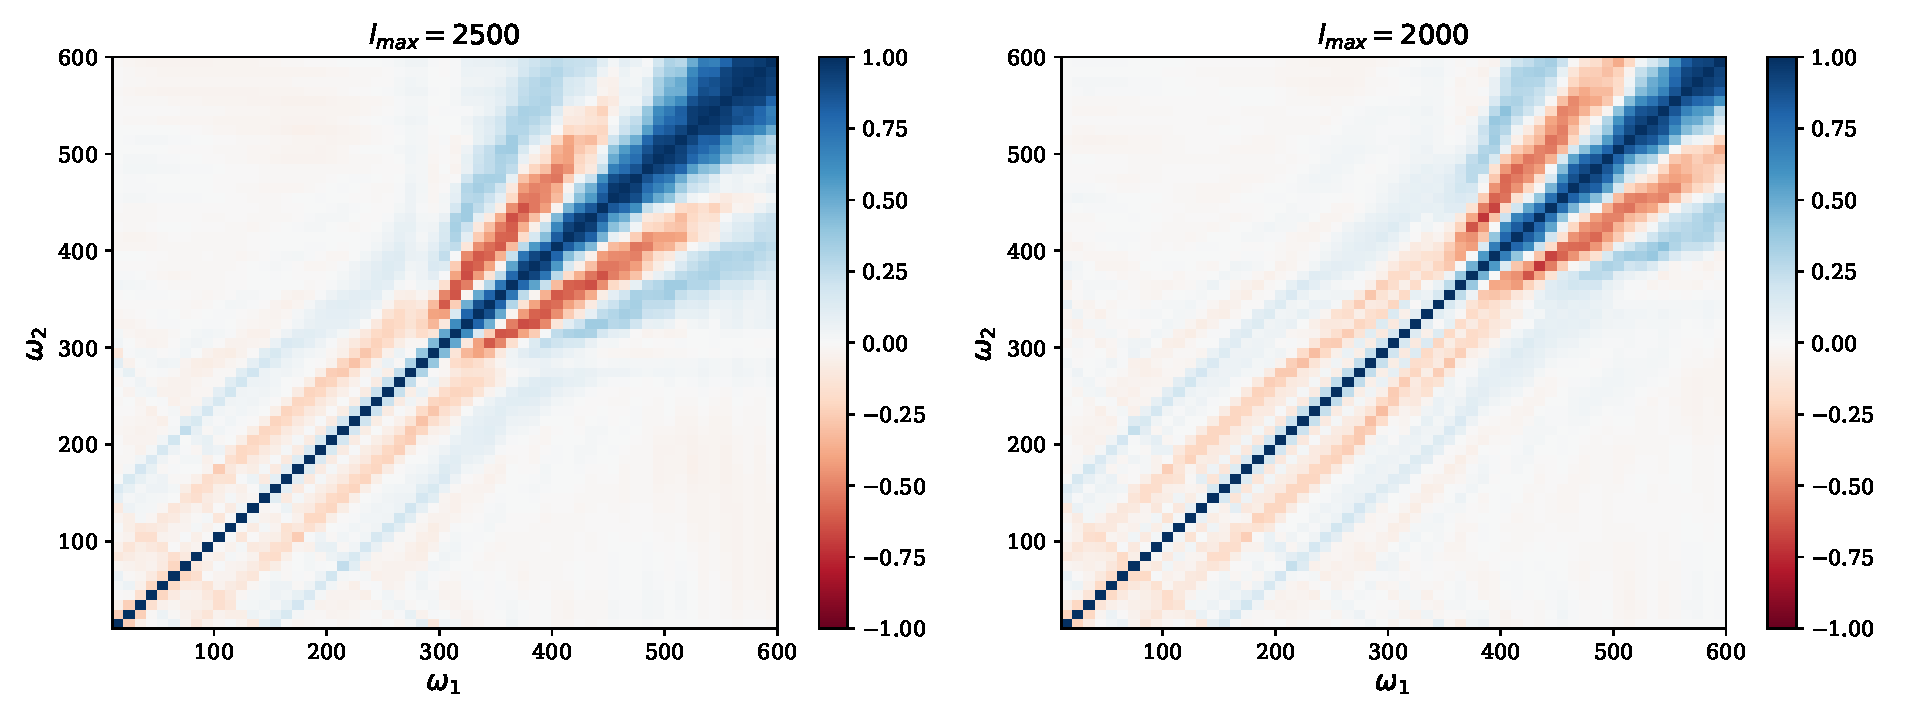
\includegraphics[width=\textwidth]{sine_template_correlations_compare_lmax_new.pdf}
	\caption{Theoretical correlations between feature model templates with different frequency $\omega$s, as described in Figure \ref{fig:feature_template_correlations}. The phase $\phi$ is set to zero in both cases, while the right plot is obtained from the Legendre basis with a different $k$ range. The maximum $l$ value is reduced from $2500$ to $2000$, shifting $(k_\text{min},k_\text{max})$ by a factor of $2000/2500 = 0.75$. Having a smaller $k$ range means fewer oscillations within the $k$ interval for same $\omega$ which provides better effective resolution. The right plot does indeed show smaller non-diagonal correlations at high frequencies.}
	\label{fig:feature_template_correlations_compare_lmax}
\end{figure}

There is a subtlety around $f_\text{NL}$ estimates obtained from inaccurate primordial basis expansions. CMB-BEst computes $\beta$s and $\Gamma$s with respect to the fixed Legendre basis, which has been shown to be accurate even for the highest degree of polynomials. When the primordial basis is unable to resolve rapid modulations as we have seen, the $f_\text{NL}$ estimates we obtain are nevertheless meaningful; they are simply probing the wrong model. The constraints are not for the given shape function, but rather its projection to the vector subspace spanned by the basis functions as shown in (\ref{eqn:primordial_basis_projection}). Detecting non-zero $f_\text{NL}$ here can still have significant implications.

Another popular template for models with oscillations is the `resonance' shape parametrised as $S(k_1, k_2, k_3) = \sin(\omega \log(k_1 + k_2 + k_3 ) + \phi)$. Log-spaced modulations are numerically harder to deal with since the oscillation frequency diverges as $k \rightarrow 0$. Note also that any scaling factors to the $k$'s can be absorbed into the phase via $\log(c(k_1 + k_2 + k_3)) = \log(k_1 + k_2 + k_3) + \log(c)$. For our Legendre basis with $k_\text{max}/k_\text{min}$ fixed to $1000$, the full $k$ range includes $\approx 1.1\omega$ oscillations. Any frequency larger than $\approx 27$ therefore cannot be expanded using $p_\text{max}=30$ polynomials. We still explore shapes with higher $\omega$s however, since the basis can pick up slower oscillations in higher $k$ values. Corresponding constraints should be taken with a grain of salt; they probe bispectrum shapes \textit{similar} to the resonance template. Low-$k$ oscillations are especially likely to be wiped out from these shapes.

Figure \ref{fig:sinlog_template_frequency_Legendre_Modal} compares $f_\text{NL}$ constraints for the resonance template over a range of $\omega$s. As can be seen from the top two plots, the signal-to-noise values obtained from the Legendre basis and Modal are relatively consistent up until $\omega \approx 35$, after which the two results start diverging significantly. The threshold is about the same for `sinlog' ($\phi = 0$) and `coslog' ($\phi=\pi/2$) shapes.

Recall that the sample $\sigma$ from $f_\text{NL}$ estimates of Gaussian simulations should converge to the theoretical value calculated from the Fisher information as $N_\text{sims}\rightarrow\infty$, since the CMB bispectrum estimator is optimal. We have checked that the sample and theoretical variances are consistent for standard templates in Section \ref{section:internal_consistency}, using both KSW and Legendre basis sets. The bottom two plots in Figure \ref{fig:sine_template_frequency_Legendre_Modal} show the equivalent results for the resonance template with varying $\omega$.

\begin{figure}[htbp!] 
	\centering    
	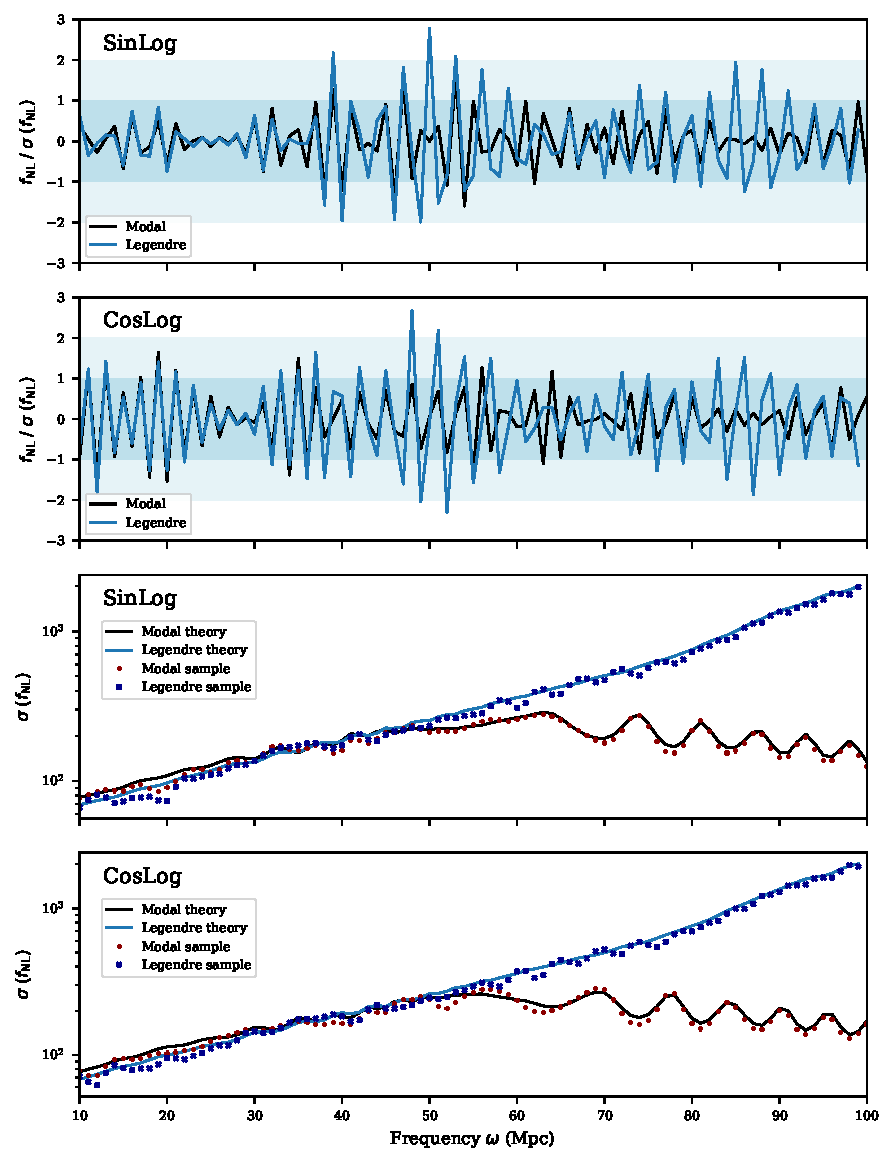
\includegraphics[width=\textwidth]{sinlog_template_frequency_Legendre_Modal.pdf}
	\caption{Constraints for the resonance shape $S(k_1,k_2,k_3) = \sin(\omega \log(k_1 + k_2 + k_3 ) + \phi)$ with varying $\omega$s and $\phi$ set to $0$ (left) and $\pi/2$ (right). Results are obtained using CMB-BEst's Legendre basis (blue) and Planck's Modal estimator (black). Top: signal-to-noise significance of the estimated $f_\text{NL}$s with $1\sigma$ and $2\sigma$ levels shaded in blue. Bottom: standard deviations of the $f_\text{NL}$ estimates against frequency $\omega$, calculated from the $f_\text{NL}$s of 140 simulations (sample) and the $\Gamma$ matrix (theory).}
	\label{fig:sinlog_template_frequency_Legendre_Modal}
\end{figure}

Similarly to the feature models studied in Chapter \ref{chapter:CMB_state-4_forecast}, uncertainty in the estimated $f_\text{NL}$s increases as we raise $\omega$, exploring more rapid oscillations in bispectrum. Both the Modal and Legendre methods lose their ability to resolve shapes with $\omega$s larger than $35$. The constraints are then no longer for the precise resonance shape but rather an approximation to it. A notable difference between Modal and CMB-BEst's Legendre basis is their behaviour at high $\omega$. Modal's numerical accuracy is completely lost after $\omega\approx 50$, leading to disproportionately large bispectra and small $\sigma$. On the other hand, Legendre retains stability in its basis expansion, yielding constraints for approximate bispectrum shapes closest to the true, high-frequency ones.

\begin{figure}[htbp!] 
	\centering    
	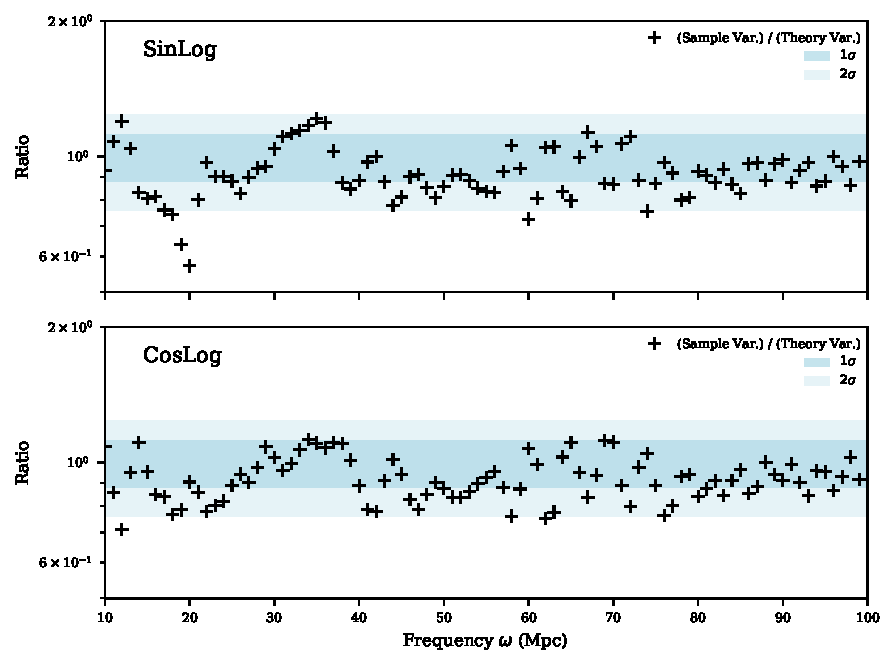
\includegraphics[width=\textwidth]{sinlog_template_frequency_variances_Legendre.pdf}
	\caption{Ratio between sample and theoretical variances obtained from Legendre basis for resonance shapes. Sampled variance is calculated from $f_\text{NL}$ estimates of $140$ Gaussian simulations. $1\sigma$ and $2\sigma$ intervals are chosen based on a $\chi^2$-distribution, which accurately describes sample variances as long as the $f_\text{NL}$s are normally distributed. Results are statistically consistent with random fluctuations except potentially at $\omega=20$, as discussed in the main text.}
	\label{fig:sinlog_template_frequency_variances_Legendre}
\end{figure}

A detailed comparison between the sample and theoretical variances is depicted in Figure \ref{fig:sinlog_template_frequency_variances_Legendre}. This serves as a useful consistency check within the CMB-BEst pipeline. Sample variances are calculated from a finite number of $f_\text{NL}$ samples from simulations. We test if these estimates are compatible with the underlying distribution: $\chi^2$ with $N_\text{sims}-1$ degrees of freedom in this case. We achieve the desired consistency for both $\phi=0$ and $\phi=\pi/2$. One potentially meaningful outlier is at $\omega=20$ and $\phi=0$, where the sample estimate is below 60\% of the expected level. This anomaly is not likely to be a numerical error specific to CMB-BEst since a similar dip can be found from Modal results in Figure \ref{fig:sinlog_template_frequency_Legendre_Modal}. No significant irregularity is found for different phases at the same frequency. We classify this point as a random fluctuation for now, but a further investigation using an independent set of Gaussian simulations is required to be certain.

As with the feature models before, we plot the correlation matrix between the templates with different $\omega$s in Figure \ref{fig:sinlog_template_correlations}. Shapes with similar $\omega$s are naturally correlated, but most off-diagonal terms of the matrix vanish. Even for $\omega > 35$ where the basis expansion becomes less accurate, cross-correlations tend to remain small until $\omega \approx 75$. We verify the stability of CMB-BEst's Legendre basis expansion; best approximations to the highly oscillatory template are found, allowing us to continue exploring independent bispectrum shapes with the characteristic log-spaced oscillations.

\begin{figure}[htbp!] 
	\centering
	(a) $ \phi=0 $
	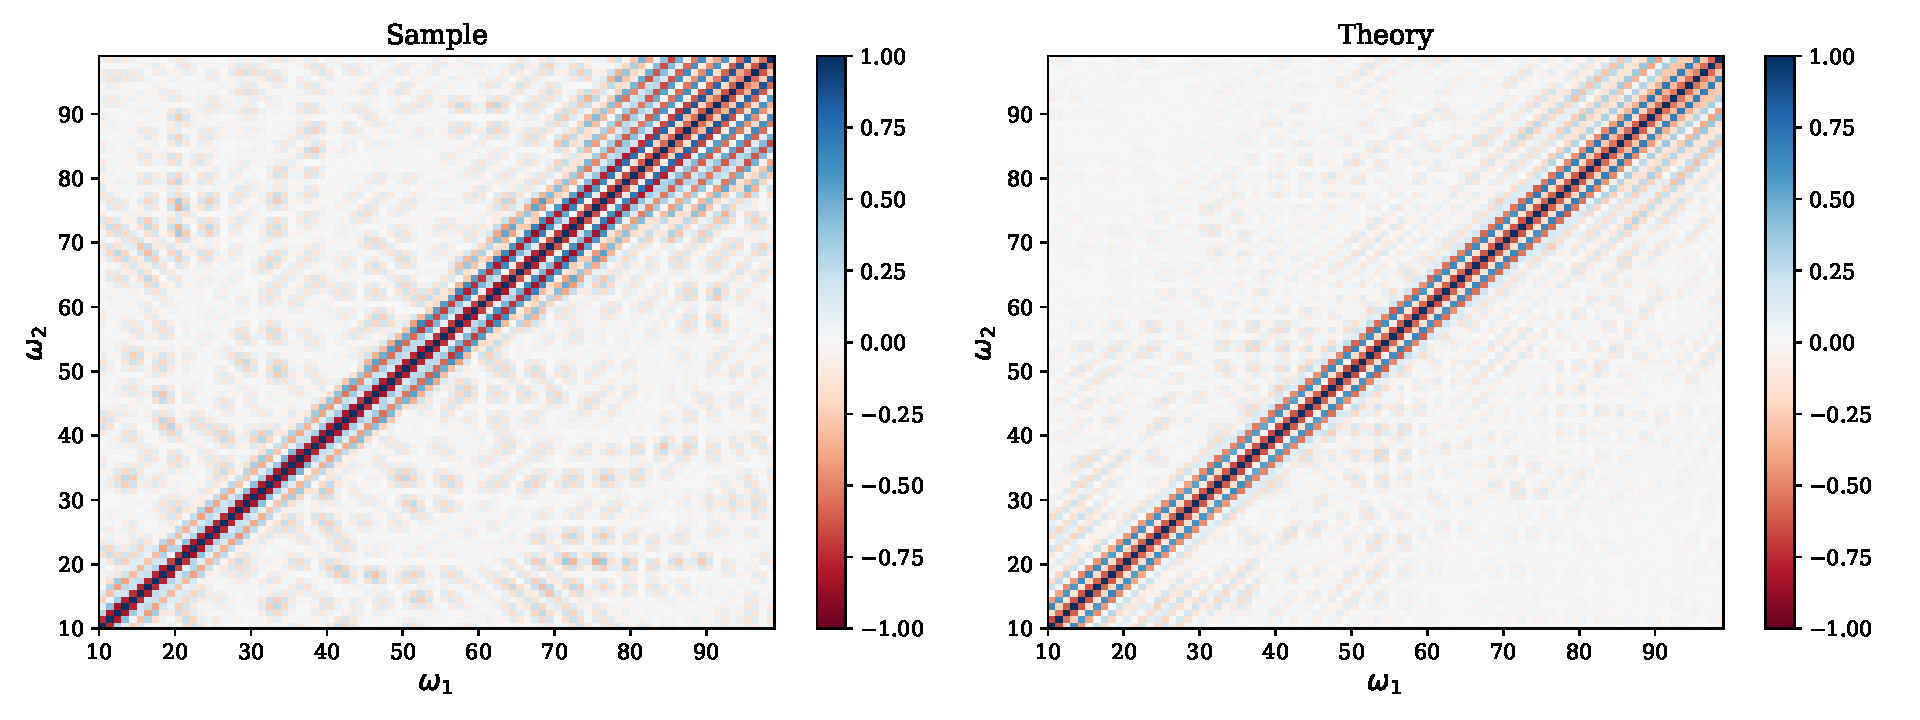
\includegraphics[width=\textwidth]{sinlog_template_correlations_new.pdf}
	(b) $ \phi=\pi/2 $
	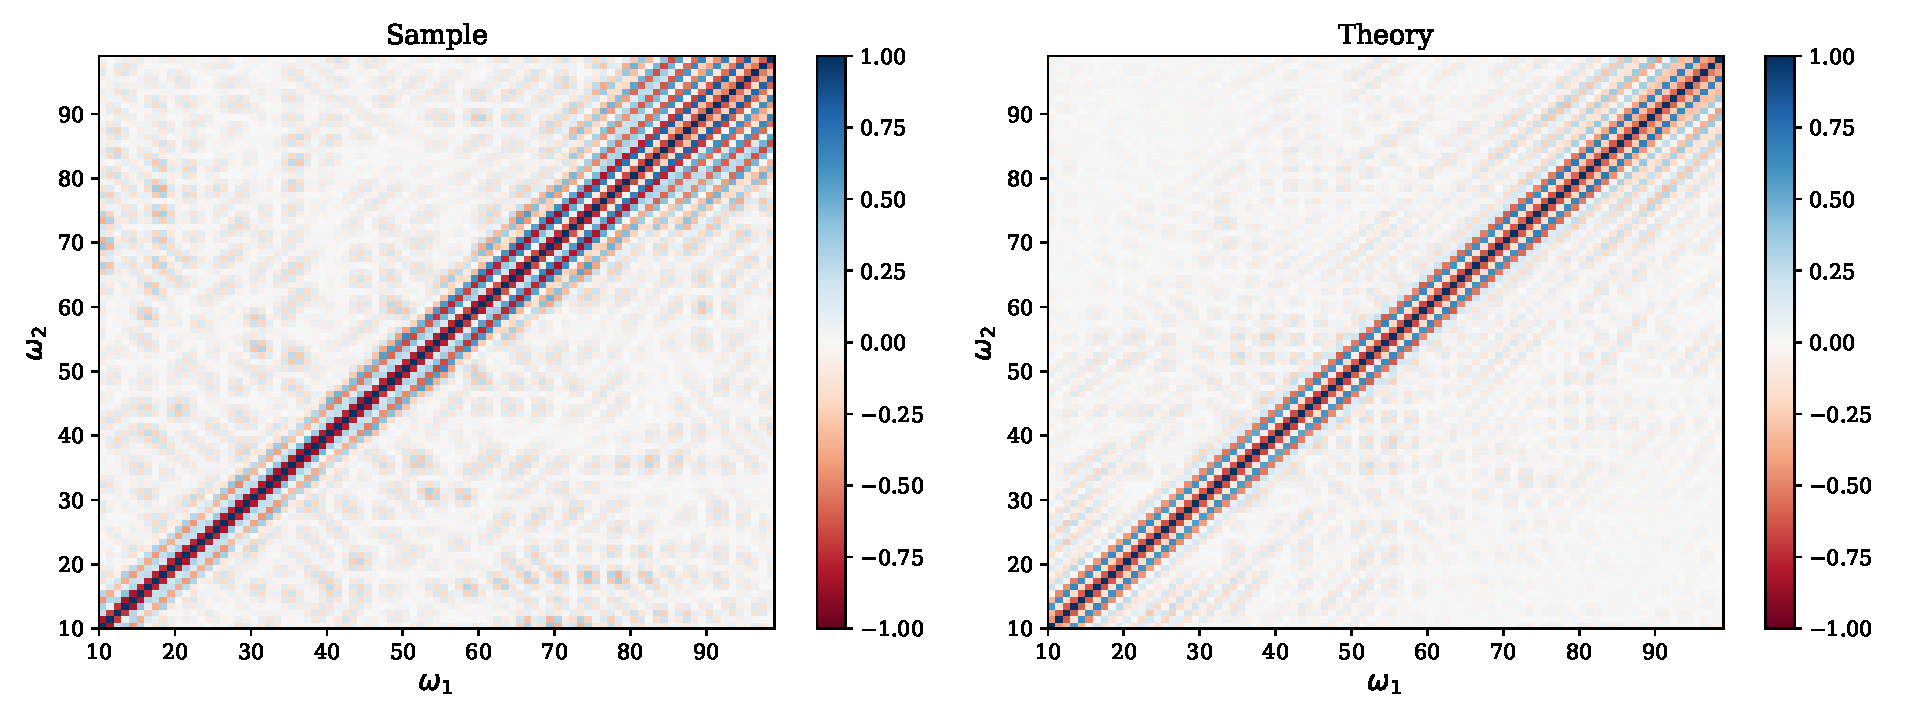
\includegraphics[width=\textwidth]{coslog_template_correlations_new.pdf}
	\caption{Correlations between resonance model templates $S(k_1,k_2,k_3) = \sin(\omega\log(k_1+k_2+k_3)+\phi)$ with different $\omega$ values, for (a) $\phi = 0$ and (b) $\phi=\pi/2$. `Sample' correlations are obtained from the Legendre basis $f_\text{NL}$ estimates from 140 Gaussian simulations. `Theory' correlations come from the inner product induced by $\Gamma$ matrix as shown in (\ref{eqn:late_time_inner_product}).}
	\label{fig:sinlog_template_correlations}
\end{figure}


\subsection{Proof of concept} \label{section:proof_of_concept}


\textsc{Primodal} is a fast and efficient numerical code for computing bispectra of primordial perturbations given a single field inflation Lagrangian using in-in formalism \cite{Clarke2021}. The computed bispectrum is expressed as coefficients of a separable basis expansion in \textsc{Primodal}, as opposed to a grid of discrete points like other in-in codes. Choosing an equivalent basis set for \textsc{CMB-BEst} therefore creates a direct link between the two codes. The combined pipeline is capable of constraining specific inflation models directly without the use of approximate templates. Such template-free bispectrum analysis also enables a fast and extensive scan of theory parameters.

Collaborating closely with the main author of \textsc{Primodal}, Philip Clarke, we verified the integrity of the combined \textsc{Primodal} + \textsc{CMB-BEst} routine. We thoroughly tested the consistency of basis functions, their orthogonalisation, and convergence. Both \textsc{Primodal} and \textsc{CMB-BEst} are now in the exploitation phase. We present a working example of the combined pipeline as a proof of concept.

DBI inflation \cite{Silverstein2004dbi,Alishahiha2004dbi,Chen2005runningdbi,Bean2008comparingdbi} is a well-studied single-field inflation model inspired by string theory. Its action follows the general form \eqref{eqn:general_single_field_action}, with a non-canonical kinetic term given by
\begin{align}
	P(X,\phi) = - \frac{1}{f(\phi)} \left[ \sqrt{1 - 2f(\phi)X} - 1 \right] - V(\phi),
\end{align}
where $X=-\frac{1}{2} g^{\mu\nu} \partial_\mu \phi \partial_\nu \phi$ as before. $f(\phi)$ is an arbitrary function called the warp factor. We choose
\begin{align}
	f(\phi) = \frac{\lambda_\text{DBI}}{\phi^4}, \qquad V(\phi) = V_0 - \frac{1}{2}m^2\phi^2, \qquad m = \sqrt{\beta_\text{IR}} \; H,
\end{align}
for some theory parameters $\lambda_\text{DBI}$, $V_0$, and $\beta_\text{IR}$. The sound speed can then be obtained from \eqref{eqn:general_single_field_sound_speed}, which evaluates to $c^\text{DBI}_\text{s} \approx 3/\beta_\text{IR} N_e$ under some slow-roll approximations \cite{Chen2005runningdbi}. Here, $N_e$ denotes the number of e-folds until the end of inflation.

DBI inflation generates non-Gaussianity with its shape similar to the equilateral template \eqref{def:equilateral_template}. The latest constraints on the model comes from the Planck CMB bispectrum analysis using an approximate template 
\begin{align}
	B_\Phi^\text{DBI}(k_1,k_2,k_3) = \frac{6A_\Phi^2}{(k_1 k_2 k_3)^3} \frac{-3/7}{(k_1 + k_2 + k_3)^2} \bigg[ \sum_i k_i^5 &+ \sum_{i\neq j} (2k_i^4 k_j - 3k_i^3 k_j^2)  \nonumber \\
	&+ \sum_{i\neq j\neq l} (k_i^3 k_j k_l - 4k_i^2 k_j^2 k_l) \bigg]. \label{eqn:dbi_bispectrum_template}
\end{align}
We switched to a convention where the potential $\Phi$ is used instead of $\zeta$. On superhorizon scales at the end of inflation they differ by a constant factor: $\Phi = (3/5)\zeta$. With respect to this template, the theoretical bispectrum from DBI inflation has amplitude
\begin{align}
	f_\text{NL}^\text{DBI} \approx - \frac{35}{108} \left[ \frac{1}{\left( c^\text{DBI}_\text{s} \right)^2} - 1 \right], \label{eqn:DBI_fNL_and_sound_speed}
\end{align}
an approximation which is accurate as long as the DBI sound speed $c^\text{DBI}_\text{s} \ll 1$. Constraints on $f_\text{NL}^\text{DBI}$ therefore place limits on $c_\text{s}$. Planck 2018 analysis \cite{PlanckCollaboration2018} found $f_\text{NL}^\text{DBI} = 46 \;\pm\; 58$ with a 68\% confidence level from CMB temperature data. The corresponding bound on the speed of sound is $c^\text{DBI}_\text{s} \ge 0.079$.

We reproduce the DBI sound speed constraint from Planck 2018 analysis using the \textsc{Primodal}$+$\textsc{CMB-BEst} routine. Unlike the Planck analysis, our method does not require templates to connect inflationary predictions to CMB data. Instead of using a single estimate from an approximate template, we scan over DBI theory parameters and constrain the individual primordial bispectrum directly. A given parameter set can be ruled out if the corresponding constraint on $f_\text{NL}$ excludes $f_\text{NL}=1$ with high confidence. 

One notable limitation in the current implementation of \textsc{Primodal} is that the details of how inflation ends are not prescribed. This means that the scales during inflation and what we observe cannot be mapped directly, which restricts our ability to translate the results into a constraint on more fundamental parameters such as $\beta_\text{IR}$. Our work here still serves as a useful validation of the combined pipeline. For the DBI sound speed scan, the approximate relation \eqref{eqn:DBI_fNL_and_sound_speed} is used to relate the output $c^*_s$\textemdash sound speed at some pivot scale during horizon crossing\textemdash from \textsc{Primodal} with the physical DBI sound speed $c^\text{DBI}_\text{s}$. Numerous other validation tests we performed such as convergence tests with respect to the basis size $p_\text{max}$ are unaffected by this caveat and still serves as a proof of concept for our combined pipeline.

The parameter $\beta_\text{IR}$ is varied within the interval $[0.1885,0.58]$ while fixing other parameters as $\lambda_\text{DBI} = 2.00475 \times 10^15$, $V_0 = 5.2 \times 10^{-12} M^4_{pl}$, and $\phi_0 = 0.46042 M_{pl}$, where $M_{pl}$ is the Planck mass. Further details of the scan will be included in \cite{Sohn2021inprep}. The results are depicted in Figure \ref{fig:dbi_sound_speed_scan}.

\begin{figure}[htbp!] 
	\centering    
	\includegraphics[width=\textwidth]{dbi_sound_speed_scan_annotated_new.pdf}
	\caption{Constraints on the DBI model with varying sound speed $c_\text{s}$. Primordial bispectrum computed from \textsc{Primodal} is fed directly into CMB-BEst in the form of coefficients $\alpha_{p_1 p_2 p_3}$ appearing in Legendre basis expansion. Constraints from the Legendre basis with $p_\text{max}=30$ (black $+$) are shown in comparison with $p_\text{max}=29$ (black $\times$). $1\sigma$ and $2\sigma$ confidence intervals around $0$ are shaded in blue and represent the uncertainty in the estimated $f_\text{NL}$s. Bispectrum shapes are normalised so that $f_\text{NL}=1$ corresponds to the DBI model under consideration. Our constraint on DBI sound speed is $c^\text{DBI}_\text{s} > 0.056$ with $95\%$ confidence level. Equivalent results from an approximate DBI bispectrum template \eqref{eqn:dbi_bispectrum_template} (blue dashed) give the $c^\text{DBI}_\text{s}$ bound identical up to two significant figures.}
	\label{fig:dbi_sound_speed_scan}
\end{figure}

First of all, we check that our Legendre basis with $p_\text{max}=30$ has converged and accurately represents the primordial bispectrum from DBI inflation. Values of the $f_\text{NL}$ estimates obtained from $p_\text{max}=30$ were tested against the equivalent result with $p_\text{max}=29$ and shown to differ by less than $0.01\%$, as can be seen in Figure \ref{fig:dbi_sound_speed_scan}. In order to thoroughly investigate the degree of convergence, we studied a late-time equivalent of $\epsilon$ in  \eqref{def:primordial_shape_epsilon} used to compare primordial bispectrum shapes;
\begin{align}
	\epsilon^2 (\vv{f}_1, \vv{f}_2) = \frac{1}{N_{sim}}  \sum_{i=1}^{N_{sim}} \left( \frac{f^{(i)}_1}{\sigma_1} - \frac{f^{(i)}_2}{\sigma_2} \right)^2,
\end{align}
where $f^{(i)}_1$ and $f^{(i)}_2$ denote $f_\text{NL}$ estimate for the $i$th Gaussian simulated map from the two routines. $\epsilon^2$ measures the mean squared error in the two sets of $f_\text{NL}$ signal-to-noises for $N_{sim}$ simulations. Comparing results from the Legendre basis with $p_\text{max} = 30$ and $25$ across the scan, we confirmed that $\epsilon < 0.01$ in the full range and $\epsilon \approx 0.002$ for the majority. A plot with the full result will be provided in \cite{Sohn2021inprep}.

Secondly, we constrain the DBI sound speed as $c_\text{s} \gtrapprox 0.056$ with $95\%$ confidence using CMB temperature data from Planck. Each of the points in Figure \ref{fig:dbi_sound_speed_scan} are normalised to some $\tilde{f}_\text{NL}$ such that $\tilde{f}_\text{NL}=1$ corresponds to the bispectrum predicted by the model. Estimates from the Planck 2018 map take negative values with error bars small enough to exclude $f_\text{NL}=1$ with $2\sigma$ confidence level when $c_\text{s} < 0.056$. Our constraint is similar but not identical to the result from Planck 2018 analysis which reads $c_\text{s} \ge 0.079$. The discrepancy stems from differences in the constraints for DBI template \eqref{eqn:dbi_bispectrum_template}: $f^\text{DBI}_\text{NL}=27 \pm 58$ for \textsc{Primodal}+\textsc{CMB-BEst} whereas $f^\text{DBI}_\text{NL}=46 \pm 58$ for Planck. This $\approx0.32\sigma$ gap in signal to noise is largely because the Modal expansion is incomplete so that the correlation between the expanded and full DBI template equals $r\approx 0.95$. As discussed in Appendix B of \cite{PlanckCollaboration2013}, this level of correlation causes an expected scatter in $f_\text{NL}$s approximately equal to $0.3\sigma$.

Lastly, we verify that the DBI template \eqref{eqn:dbi_bispectrum_template} accurately approximates the full numerical result obtained from \textsc{Primodal}. Shown in blue dashed line on Figure \ref{fig:dbi_sound_speed_scan}, the difference between $\tilde{f}_\text{NL}$ constraints obtained using \textsc{Primodal} and the DBI template differ by order $O(0.01)\sigma$.

\bigskip

We extend the \textsc{Primodal}+\textsc{CMB-BEst} pipeline to study DBI models with resonance. The primordial bispectrum appears similar to the DBI template but has extra log-spaced oscillations superimposed. The Planck analysis covers both DBI shape and resonance templates independently but has not constrained the combination of the two. Our method studies the bispectrum obtained directly from inflation without using approximate templates. We vary the effective frequency $\omega$ of the oscillations while keeping other DBI theory parameters fixed. Figure \ref{fig:dbi_resonance_scan} summarises the results of the scan.

\begin{figure}[htbp!] 
	\centering    
	\includegraphics[width=0.8\textwidth]{dbi_reso_scan_fNLs_new.pdf}
	\caption{Constraints on the DBI model with oscillations imposed on the inflationary potential, causing resonance-type bispectra approximately parametrised as $\sin(\omega \log(k_1+k_2+k_3) + \phi)$. The primordial bispectrum computed from \textsc{Primodal} for various oscillation frequency $\omega$ has been fed directly to CMB-BEst. The results (black line) are shown together with the ones obtained from a smaller basis where $p_\text{max}=29$ (blue $\times$). The blue regions in the plot represent $1\sigma$ and $2\sigma$ confidence intervals.}
	\label{fig:dbi_resonance_scan}
\end{figure}

We find no significant detection of non-Gaussianity in the parameter range we study. Note also that our $f_\text{NL}$ estimates become unreliable after $\omega\gtrsim2.0$ as the Legendre basis fails to represent rapid oscillations accurately. This can be seen by comparing the estimates from bases of size $p_\text{max}=30$ and $29$ in the figure. Augmenting the Legendre basis with specific functions or choosing an alternative set of basis \cite{Clarke2021} can improve the convergence up to $\omega\approx5$ (to be included in \cite{Sohn2021inprep}), which is a significant improvement but still rather restrictive compared to the viable parameter range of $\omega\lesssim 35$ for the `vanilla' resonance models shown in Figure \ref{fig:sinlog_template_frequency_Legendre_Modal}.

Investigating the lack of convergence has revealed a more fundamental issue with the primordial basis expansion. Earlier in this chapter, we discussed how the tetrapyd domain of primordial bispectrum can be extended to the cube given by $[k_\text{min},k_\text{max}]^3$ such that the decomposition coefficients can be computed accurately and efficiently via \eqref{eqn:basis_expansion}. By doing so, we are expanding the given bispectrum in a cube which contains the tetrapyd while analytically continuing the function in between the two. Having good convergence in the cube then implies good convergence in the tetrapyd inside it. However, in cases where the target function behaves badly outside the tetrapyd, trying to fit the function in the whole cube instead of the tetrapyd may be suboptimal.

We demonstrate this issue by computing the $f_\text{NL}$ constraints using a bispectrum template $S(k_1,k_2,k_3) = S^\text{equil}(k_1,k_2,k_3) \sin(\omega \log(k_1+k_2+k_3))$: the equilateral shape with sine-log oscillations imposed. Figure \ref{fig:sinlog_equil_template_decomp_comparison} shows two plots analogous to Figure \ref{fig:sinlog_template_correlations}. The correlations between $f_\text{NL}$s estimated from different values of $\omega$ are computed using two different approaches for the primordial basis expansion. Shown on the left hand side is the result for when we evaluate the given shape function $S(k_1,k_2,k_3)$ within the whole \textit{cube}, as we have so far. We see that the basis fails to express the given bispectrum template accurately after $\omega\gtrsim4$. Large correlations shown in the plot are simply artefacts of inaccuracy in the expansion.

\begin{figure}[htbp!] 
	\centering    
	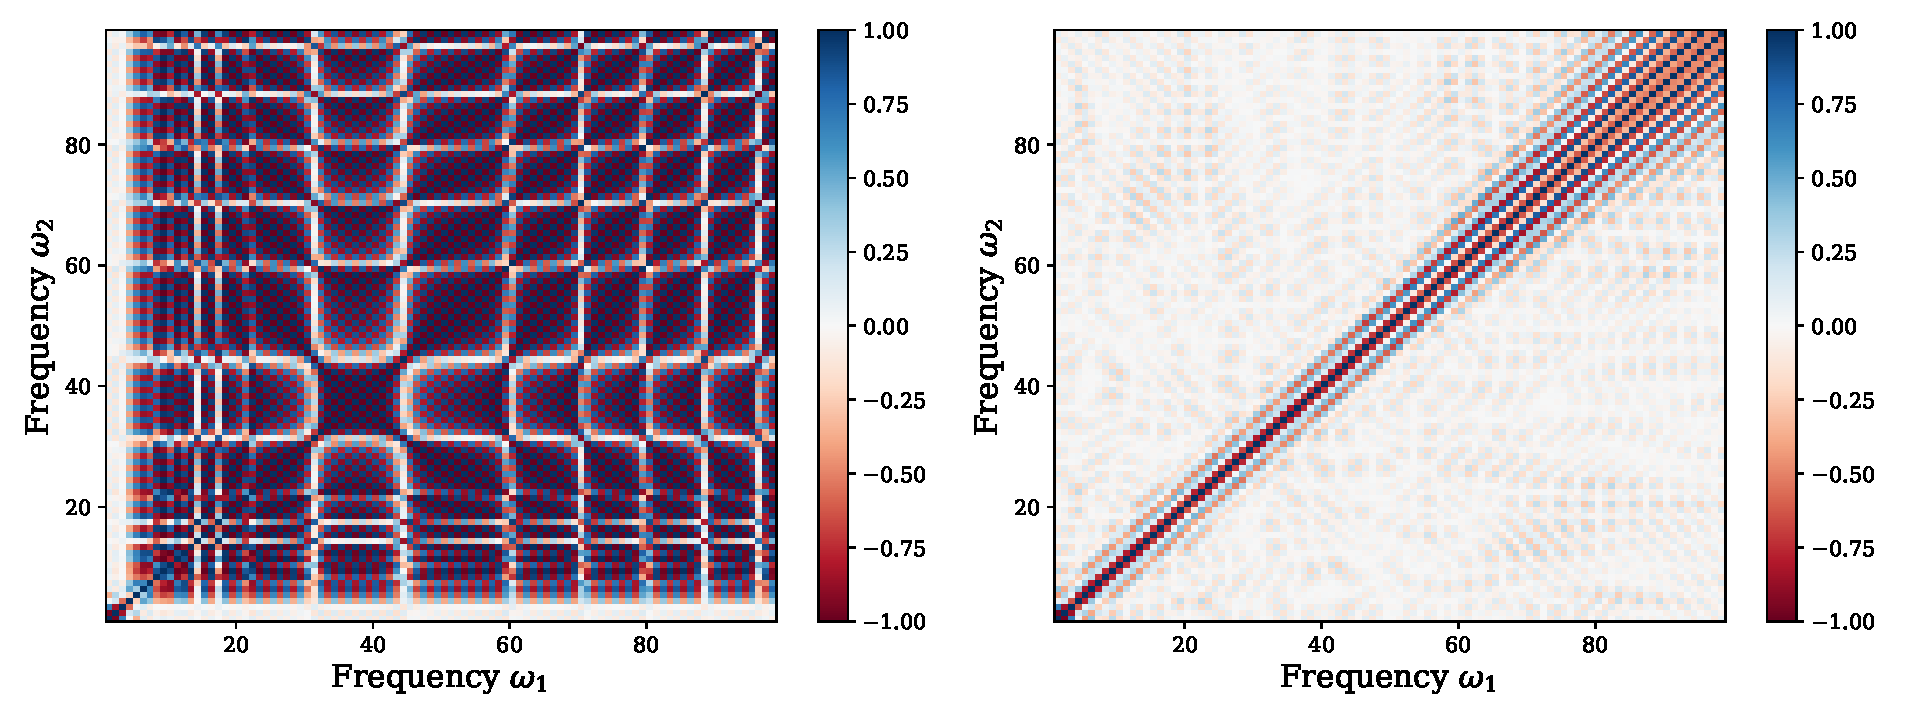
\includegraphics[width=\textwidth]{sinlog_equil_template_correlations_compare_decomp.pdf}
	\caption{Correlations between $f_\text{NL}$ constraints for the enveloped resonance shape $S(k_1,k_2,k_3) = S^\text{equil}(k_1,k_2,k_3) \sin(\omega \log(k_1+k_2+k_3))$ with different $\omega$s. Since the given shape behaves badly in the region outside the tetrapyd but within the cubic domain of (\ref{eqn:basis_expansion}), we observe large off-diagonal correlations in the original Legendre basis expansion (Left). Manually setting the shape function to zero at these unphysical configurations therefore dramatically improves numerical performance (Right). }
	\label{fig:sinlog_equil_template_decomp_comparison}
\end{figure}

On the right hand side is the result for which the shape function values outside the tetrapyd were manually set to zero during the primordial basis expansion. The modified shape function is still continuous within the cubic domain since the equilateral shape, despite its divergence outside the tetrapyd, vanishes on the boundaries of it. We see that this simple trick has dramatically improved the basis' ability to expand highly oscillatory bispectrum templates. The cross-correlations between templates remain small up until $\omega\approx75$, quite similar to what we saw for the sine-log templates. We confirm that it is indeed the bad behaviour of the templates outside the tetrapyd domain during the primordial basis expansion that causes the lack of convergence. We plan to explore this topic further in the future.

\newpage
\section*{Summary}

In this chapter, we presented a thorough review of our work on the high-resolution bispectrum estimator \textsc{CMB-BEst}. Starting with the mathematical framework of our pipeline, we showed that our formalism combines the strengths of conventional approaches to bispectrum estimation; we can handle highly oscillatory functions as accurately as the KSW estimator whilst covering a broad range of models like Modal. In order to tackle the computational complexity, we thoroughly optimised the code in both algorithmic and implementation levels. The code was then parallelised for maximal utilisation of high performance computing clusters.

With the completed code we performed various tests to validate the integrity of \textsc{CMB-BEst}. We showed that the two different choices of basis functions\textemdash monomials and Legendre polynomials\textemdash give consistent constraints for the standard bispectrum shapes. Furthermore, we compared our results to those from the Modal estimator using the Planck 2018 data and found that they agree on a map-by-map basis. Oscillatory shapes such as the feature and resonance templates were also constrained; by analysing correlation between the templates with different oscillation frequencies, we showed that our basis can handle oscillatory shapes as accurately as the Planck analysis using the Legendre basis of size $p_\text{max}=30$.

Having validated the pipeline, we provided a proof-of-concept example where \textsc{CMB-BEst} is combined with \textsc{Primodal} to constrain inflation models with non-canonical kinetic terms. The combined pipeline is capable of constraining inflation models directly without using approximate templates. We studied the DBI inflation models while varying the speed of sound parameter to obtain the constraint $c_\text{s}^\text{DBI} \ge 0.056$ with 95\% confidence. We are currently preparing to publish the work presented here as \cite{Sohn2021inprep}.





% Old table
%\begin{table}[h]
%	\caption{Constraints for the standard templates for the KSW and Legendre basis from CMB-BEst, in comparison with the `Modal' pipeline from Planck 2018 analysis \cite{PlanckCollaboration2018}}
%	\centering
%	\label{table:trio_fNL_comparison_with_planck}
%	\renewcommand{\arraystretch}{1.5} 
%	\begin{tabular}{llrrr}
%		\toprule
%		Template & Estimator &  $f_\text{NL}^T$ &  $\bar{\sigma}^T$ &  $\sigma^T$ \\
%		\toprule
%		
%		Local & KSW &   -2.2 &      5.5 &      5.3 \\
%		& Legendre &   -2.0 &      5.9 &      5.7 \\
%		& Modal &   -0.6 &      6.4 &      6.1 \\
%		
%		\midrule
%		Equilateral & KSW &   16.7 &     61.1 &     67.7 \\
%		& Legendre &   15.2 &     61.7 &     67.7 \\
%		& Modal &   33.8 &     66.5 &     72.4 \\
%		
%		\midrule
%		Orthogonal & KSW &   -6.9 &     37.6 &     33.7 \\
%		& Legendre &   -8.5 &     38.0 &     33.9 \\
%		& Modal &  -26.5 &     42.8 &     39.3 \\
%		\bottomrule
%	\end{tabular}
%\end{table}

%!TEX root = ../thesis.tex
%*******************************************************************************
%****************************** Sixth Chapter **********************************
%*******************************************************************************
\chapter{Conclusion}

The standard model of cosmology has been remarkably successful; the CMB power spectrum from Planck, for example, shows an exquisite fit to the $\Lambda$CDM model with only six free parameters. There are many unanswered questions remaining, however, especially regarding the early universe physics. The most widely accepted theory for the early universe is inflation, whose prediction of the scale-invariant primordial spectra has been tested to be consistent with the observed data. Inflation also resolves the horizon and flatness problems present in the vanilla Big Bang cosmology. The simplest scenario of the single-field slow-roll inflation with a canonical kinetic term can explain the current observations, but there are also numerous other physically well-motivated scenarios that are yet to be ruled out.

The key to distinguishing different models of inflation is primordial non-Gaussianity. Deviations from the most canonical inflation model leave weak non-Gaussian signatures in the primordial perturbations. These imprints are best captured in the bispectrum of the primordial perturbations. Studying the shape and amplitude of the primordial bispectrum therefore allows us to constrain various inflation models directly. The CMB is the ideal probe for this job since its anisotropy depends linearly on the initial density perturbations. The CMB bispectrum hence directly relates to the primordial bispectrum and is used to construct the optimal estimator for the primordial non-Gaussianity parameter $f_\text{NL}$. 

The most recent Planck analysis has constrained $f_\text{NL}$ to great precision using the CMB bispectrum estimator. No primordial source of non-Gaussianity has been found, and $f_\text{NL}$s for the standard shapes are currently consistent with $0$. More interesting `hints' of non-Gaussianity have been found in models with oscillations in the bispectrum. Signals of $3$-$4\sigma$ significance have been found in these models, but scanning over a large parameter space meant that these are not yet conclusive detections. A further investigation using independent and more precise measurements would be extremely beneficial.

The next generation of CMB experiments is anticipated to measure the polarisation of the CMB with greatly enhanced sensitivity. Given that the Planck constraints on oscillatory models benefited much more from the inclusion of polarisation data than other shapes, we predict that the constraining power would benefit immensely from the future CMB data. Our work presented in Chapter 4 forecasts that the most sensitive CMB Stage-4 experiment specification is expected to yield a factor of 1.7-2.2 times more stringent constraints compared to Planck.

Despite the bright prospects and growing interest in constraining oscillatory models, a large part of the model and parameter space are currently unconstrained due to numerical and computational difficulties. The CMB bispectrum estimation is a challenging task where the na\"ive computation is practically impossible. There are two main approaches to this: KSW and Modal. The KSW estimator exploits the inherent separability of the primordial bispectrum template to efficiently compute the multi-dimensional integrals involved. This method can accurately constrain even highly oscillatory shapes but is severely restrictive in the type of bispectrum shapes it can handle. On the other hand, the Modal estimator expands the primordial and late-time bispectra in terms of separable mode functions to tackle the problem. The Modal code is heavily optimised and can constrain a wide range of non-separable shapes. However, the Modal estimator has trouble dealing with high-frequency oscillations, since the basis expansion struggles to converge. Choosing a specialised basis set to handle oscillations is also complicated by the fact that there are two separate basis sets\textemdash primordial and late-time\textemdash to consider.

Our novel approach to the CMB bispectrum estimation, \textsc{CMB-BEst}, is designed to combine the strengths of the KSW and Modal estimators, and hence is suitable for constraining general oscillatory models using future CMB data. We use the primordial basis expansion to decompose the given bispectrum shape into separable terms and then apply a KSW-like method to obtain constraints on each of them. \textsc{CMB-BEst} works for general basis sets and is in fact equivalent to the KSW estimator for a simple choice of basis. It can handle high-frequency oscillations as accurately as the KSW estimator and applies to general non-separable shapes like the Modal estimator.

There is no free lunch, however. The \textsc{CMB-BEst} pipeline is computationally more costly than both the KSW and Modal ones. We therefore invested a significant amount of time optimising the code at both algorithmic and implementation levels. The code was then parallelised on multiple levels to fully benefit from the modern computing architecture. The total runtime has improved many orders of magnitude over the course of this process. The completed code has then thoroughly tested against the Modal pipeline used in the Planck 2018 analysis. We found that the results are consistent with Planck map-by-map using 140 simulated maps, for the standard shapes as well as the feature and resonance templates.

\textsc{CMB-BEst} has been validated and is now in the exploitation phase. Working in collaboration with the authors of \textsc{Primodal}, we developed a fluid pipeline where a given inflationary Lagrangian can be directly constrained without the use of approximate templates. This allows a fast and accurate constraint to the specific model under consideration. As a proof-of-concept example, we presented work on constraining the DBI sound speed in Chapter 5, where we obtained $c_\text{s}^\text{DBI} \ge 0.056$ with 95\% confidence. The combined \textsc{Primodal}+\textsc{CMB-BEst} pipeline can perform similar scans on other theoretical parameters, which we plan to do in the near future.

There are currently two main routes for improvement for \textsc{CMB-BEst}. First, the code can be generalised to incorporate the E-mode polarisation data. Implementing this should be straightforward using an orthonormalisation defined in Chapter 4. The additional computational complexity involved in the extra set of spherical harmonic transforms for polarisation is expected to be subdominant and have a small impact overall. Second, we plan on improving the current method used for the decomposition of a given primordial shape function. We will investigate further the effect of the integration domain, as we saw from the example of the DBI resonance models in Chapter 5.

It is truly an exciting time to be researching cosmology. Numerous future experiments will soon provide us with ever more immense and accurate measurements of the observable universe. We believe that the work presented here will add to the community's continued efforts to better understand the universe we live in.
%\include{Chapter7/chapter7}



% ********************************** Back Matter *******************************
% Backmatter should be commented out, if you are using appendices after References
%\backmatter

% ********************************** Bibliography ******************************
\begin{spacing}{0.9}

% To use the conventional natbib style referencing
% Bibliography style previews: http://nodonn.tipido.net/bibstyle.php
% Reference styles: http://sites.stat.psu.edu/~surajit/present/bib.htm

\bibliographystyle{apalike}
%\bibliographystyle{unsrt} % Use for unsorted references  
%\bibliographystyle{plainnat} % use this to have URLs listed in References
\cleardoublepage
\bibliography{References/references} % Path to your References.bib file


% If you would like to use BibLaTeX for your references, pass `custombib' as
% an option in the document class. The location of 'reference.bib' should be
% specified in the preamble.tex file in the custombib section.
% Comment out the lines related to natbib above and uncomment the following line.

%\printbibliography[heading=bibintoc, title={References}]


\end{spacing}

% ********************************** Appendices ********************************

\begin{appendices} % Using appendices environment for more functunality

%%!TEX root = ../thesis.tex
% ******************************* Thesis Appendix A ****************************
\chapter{How to install \LaTeX} 

\section*{Windows OS}

\subsection*{TeXLive package - full version}
\begin{enumerate}
\item	Download the TeXLive ISO (2.2GB) from\\
\href{https://www.tug.org/texlive/}{https://www.tug.org/texlive/}
\item	Download WinCDEmu (if you don't have a virtual drive) from \\
\href{http://wincdemu.sysprogs.org/download/}
{http://wincdemu.sysprogs.org/download/}
\item	To install Windows CD Emulator follow the instructions at\\
\href{http://wincdemu.sysprogs.org/tutorials/install/}
{http://wincdemu.sysprogs.org/tutorials/install/}
\item	Right click the iso and mount it using the WinCDEmu as shown in \\
\href{http://wincdemu.sysprogs.org/tutorials/mount/}{
http://wincdemu.sysprogs.org/tutorials/mount/}
\item	Open your virtual drive and run setup.pl
\end{enumerate}

or

\subsection*{Basic MikTeX - \TeX~ distribution}
\begin{enumerate}
\item	Download Basic-MiK\TeX (32bit or 64bit) from\\
\href{http://miktex.org/download}{http://miktex.org/download}
\item	Run the installer 
\item	To add a new package go to Start >> All Programs >> MikTex >> Maintenance (Admin) and choose Package Manager
\item	Select or search for packages to install
\end{enumerate}

\subsection*{TexStudio - \TeX~ editor}
\begin{enumerate}
\item	Download TexStudio from\\
\href{http://texstudio.sourceforge.net/\#downloads}
{http://texstudio.sourceforge.net/\#downloads} 
\item	Run the installer
\end{enumerate}

\section*{Mac OS X}
\subsection*{MacTeX - \TeX~ distribution}
\begin{enumerate}
\item	Download the file from\\
\href{https://www.tug.org/mactex/}{https://www.tug.org/mactex/}
\item	Extract and double click to run the installer. It does the entire configuration, sit back and relax.
\end{enumerate}

\subsection*{TexStudio - \TeX~ editor}
\begin{enumerate}
\item	Download TexStudio from\\
\href{http://texstudio.sourceforge.net/\#downloads}
{http://texstudio.sourceforge.net/\#downloads} 
\item	Extract and Start
\end{enumerate}


\section*{Unix/Linux}
\subsection*{TeXLive - \TeX~ distribution}
\subsubsection*{Getting the distribution:}
\begin{enumerate}
\item	TexLive can be downloaded from\\
\href{http://www.tug.org/texlive/acquire-netinstall.html}
{http://www.tug.org/texlive/acquire-netinstall.html}.
\item	TexLive is provided by most operating system you can use (rpm,apt-get or yum) to get TexLive distributions
\end{enumerate}

\subsubsection*{Installation}
\begin{enumerate}
\item	Mount the ISO file in the mnt directory
\begin{verbatim}
mount -t iso9660 -o ro,loop,noauto /your/texlive####.iso /mnt
\end{verbatim}

\item	Install wget on your OS (use rpm, apt-get or yum install)
\item	Run the installer script install-tl.
\begin{verbatim}
	cd /your/download/directory
	./install-tl
\end{verbatim}
\item	Enter command `i' for installation

\item	Post-Installation configuration:\\
\href{http://www.tug.org/texlive/doc/texlive-en/texlive-en.html\#x1-320003.4.1}
{http://www.tug.org/texlive/doc/texlive-en/texlive-en.html\#x1-320003.4.1} 
\item	Set the path for the directory of TexLive binaries in your .bashrc file
\end{enumerate}

\subsubsection*{For 32bit OS}
For Bourne-compatible shells such as bash, and using Intel x86 GNU/Linux and a default directory setup as an example, the file to edit might be \begin{verbatim}
edit $~/.bashrc file and add following lines
PATH=/usr/local/texlive/2011/bin/i386-linux:$PATH; 
export PATH 
MANPATH=/usr/local/texlive/2011/texmf/doc/man:$MANPATH;
export MANPATH 
INFOPATH=/usr/local/texlive/2011/texmf/doc/info:$INFOPATH;
export INFOPATH
\end{verbatim}
\subsubsection*{For 64bit OS}
\begin{verbatim}
edit $~/.bashrc file and add following lines
PATH=/usr/local/texlive/2011/bin/x86_64-linux:$PATH;
export PATH 
MANPATH=/usr/local/texlive/2011/texmf/doc/man:$MANPATH;
export MANPATH 
INFOPATH=/usr/local/texlive/2011/texmf/doc/info:$INFOPATH;
export INFOPATH

\end{verbatim}



%\subsection{Installing directly using Linux packages} 
\subsubsection*{Fedora/RedHat/CentOS:}
\begin{verbatim} 
sudo yum install texlive 
sudo yum install psutils 
\end{verbatim}


\subsubsection*{SUSE:}
\begin{verbatim}
sudo zypper install texlive
\end{verbatim}


\subsubsection*{Debian/Ubuntu:}
\begin{verbatim} 
sudo apt-get install texlive texlive-latex-extra 
sudo apt-get install psutils
\end{verbatim}

%%!TEX root = ../thesis.tex
% ******************************* Thesis Appendix B ********************************

\chapter{Installing the CUED class file}

\LaTeX.cls files can be accessed system-wide when they are placed in the
<texmf>/tex/latex directory, where <texmf> is the root directory of the user’s \TeX installation. On systems that have a local texmf tree (<texmflocal>), which
may be named ``texmf-local'' or ``localtexmf'', it may be advisable to install packages in <texmflocal>, rather than <texmf> as the contents of the former, unlike that of the latter, are preserved after the \LaTeX system is reinstalled and/or upgraded.

It is recommended that the user create a subdirectory <texmf>/tex/latex/CUED for all CUED related \LaTeX class and package files. On some \LaTeX systems, the directory look-up tables will need to be refreshed after making additions or deletions to the system files. For \TeX Live systems this is accomplished via executing ``texhash'' as root. MIK\TeX users can run ``initexmf -u'' to accomplish the same thing.

Users not willing or able to install the files system-wide can install them in their personal directories, but will then have to provide the path (full or relative) in addition to the filename when referring to them in \LaTeX.



\end{appendices}

% *************************************** Index ********************************
\printthesisindex % If index is present

\end{document}
